\pdfoutput=1
\documentclass[]{fairmeta}
% ################# PACKAGES ###########################
\usepackage[round,authoryear]{natbib}
\usepackage{hyperref}
\usepackage[nameinlink,noabbrev]{cleveref}
\usepackage{colortbl}
\usepackage{nicematrix}
% Define our command before loading amssymb
\usepackage{amssymb}
\usepackage{amsmath}
\usepackage{adjustbox}
\usepackage{soul}
\usepackage[inline]{enumitem}
\usepackage{booktabs}
\usepackage{color}
\usepackage{xcolor}
\usepackage{bbding}
\usepackage{listings}
\usepackage{multicol}
\usepackage{xspace}
\usepackage{lmodern}
\usepackage{tablefootnote}
\usepackage{float}
\usepackage{titletoc}
\usepackage[ruled,vlined]{algorithm2e}

\crefname{algocf}{Algorithm}{Algorithms}
\Crefname{algocf}{Algorithm}{Algorithms}

% \renewcommand{\lstlistingname}{Table} % Change "Listing" to "Table"
\makeatletter
\AtBeginDocument{
\renewcommand{\sectionautorefname}{Section}
\renewcommand{\subsectionautorefname}{Section}
\renewcommand{\subsubsectionautorefname}{Section}
\renewcommand{\appendixautorefname}{Appendix}
}
\newcommand\authorNewLine[2][]{
  \addtolist[#1]{#2}{\authorlist}{\authorformat}{\\ }%
}
\newcommand\affiliationNewLine[2][]{%
  \addtolist[#1]{#2}{\affiliationlist}{\affiliationformat}{\\ }%
}
\makeatother
% \let\subsectionautorefname\sectionautorefname
% \let\subsubsectionautorefname\sectionautorefname

\lstdefinestyle{pythonstyle}{
    language=Python,
    basicstyle=\ttfamily\footnotesize,
    keywordstyle=\color{blue},
    stringstyle=\color{red!60!black},
    commentstyle=\color{gray}\itshape,
    showstringspaces=false,
    breaklines=true,
    frame=single,
    tabsize=2
}
\lstset{style=pythonstyle}
\lstdefinelanguage{Diff}{
  sensitive=false,
  morekeywords={diff,index,---,+++},               % keywords
  morecomment=[f][\color{red!80!black}]{-},         % lines beginning with '-'
  morecomment=[f][\color{green!60!black}]{+},       % lines beginning with '+'
}
\lstdefinestyle{diffstyle}{
  language=Diff,
  basicstyle=\ttfamily\scriptsize,
  columns=fullflexible,
  frame=single,
  rulecolor=\color{gray!50},
  backgroundcolor=\color{black!2},
  breaklines=true,
  breakatwhitespace=true,
  postbreak=\mbox{\textcolor{gray}{$\hookrightarrow$}\space},
  xleftmargin=1em,
  xrightmargin=1em,
  aboveskip=0.5em,                        % less vertical padding
  belowskip=0.5em,
  commentstyle=\itshape,                  % context lines
  keywordstyle=\bfseries\color{blue!70!black}, % diff/index/@@...
}
\lstset{style=diffstyle}

% Option "twocolumn" available, but please prioritize single-column

% \title{{\ha}:\newline Self-Referential Self-Improving Agents}
\title{{\ha}}

\author[1,2\dagger]{Jenny Zhang}
\author[3\dagger]{Bingchen Zhao}
\author[4,6]{Wannan Yang}
\author[6]{Jakob Foerster}
\authorNewLine[1,2,5]{Jeff Clune}
\author[\ddagger]{Minqi Jiang}
\author[7]{Sam Devlin}
\author[6]{Tatiana Shavrina}

\affiliation[1]{University of British Columbia}
\affiliation[2]{Vector Institute}
\affiliation[3]{University of Edinburgh}
\affiliationNewLine[4]{New York University}
\affiliation[5]{Canada CIFAR AI Chair}
\affiliation[6]{FAIR at Meta}
\affiliation[7]{Meta Superintelligence Labs}

\contribution[\dagger]{Work done during internship at Meta}
\contribution[\ddagger]{Work done at Meta}
% \contribution[\ddagger]{Middle authors are listed in alphabetical order}
% \contribution[\ddagger]{Joint last authors}

\abstract{
Self-improving AI systems aim to reduce reliance on human engineering by learning to improve their own learning and problem-solving processes. Existing approaches to recursive self-improvement typically rely on fixed, handcrafted meta-level mechanisms, which fundamentally limit how fast such systems can improve. We introduce \textbf{HyperAgents}, which can in principle carry out self-referential self-improvement on any computable task. A hyperagent unifies a \textit{task agent} and a \textit{meta agent} within a single modifiable program, enabling metacognitive self-modification, in which the hyperagent improves not only how it solves tasks (i.e., improving the task agent), but also how it performs future self-improvements (i.e., improving the meta agent). We realize this within the \textbf{Open-ended Hyperagent Machine} (OHM), where a single initialized hyperagent evolves through open-ended exploration by repeatedly generating and evaluating self-modified variants, forming a growing archive of stepping stones for future improvement. This process allows improvements to accumulate over time rather than converge prematurely. Across diverse domains (i.e., coding, paper review, robotics reward design, and Olympiad-level math grading), the OHM consistently improves task performance over time and outperforms baselines without self-improvement or open-ended exploration, as well as prior self-improving systems (e.g., the Darwin G\"odel Machine). We further show that the OHM improves the process by which it generates new agents, since these meta-level improvements (e.g., persistent memory, performance tracking) transfer across domains and accumulate over different runs. All experiments were conducted with safety precautions (e.g., sandboxing, human oversight). We extensively discuss what safety entails in this setting and the broader implications of self-improving systems. HyperAgents offer a glimpse of open-ended AI systems that do not merely search for better solutions, but continually improve the search for new improvements.
}

\date{\today}
\correspondence{Jenny Zhang at \email{jennyzzt@cs.ubc.ca}, Tatiana Shavrina at \email{rybolos@meta.com}}

% You can add additional metadata fields as follows 
\metadata[Code]{\url{https://github.com/facebookresearch/HyperAgents}}
% \metadata[Blogpost]{\url{https://ai.meta.com/blog/?page=1}}


\newif\ifcomment
\commenttrue % enable comments
% \commentfalse
\newcommand{\jz}[1]{\textcolor{olive}{(\ifcomment JZ: #1\else\fi)}}
\newcommand{\jzsout}[1]{\textcolor{olive}{\ifcomment JZ: \sout{#1}\else\fi}}
\newcommand{\ts}[1]{\textcolor{blue}{(\ifcomment TS: #1\else\fi)}}
\newcommand{\tssout}[1]{\textcolor{blue}{\ifcomment TS: \sout{#1}\else\fi}}
\newcommand{\jc}[1]{\textcolor{blue}{(\ifcomment JC: #1\else\fi)}}
\newcommand{\jcsout}[1]{\textcolor{blue}{\ifcomment JC: \sout{#1}\else\fi}}
\newcommand{\todo}[1]{\textcolor{red}{\ifcomment(\textbf{TODO}: #1)\else\fi}}


\newcommand{\ha}{\fontfamily{lmr}\selectfont\mdseries\textsc{HyperAgents}\xspace}

\begin{document}

\maketitle

\section{Introduction}
\label{sec:intro}

With appropriate safety considerations, AI systems that can improve themselves could transform scientific progress from a human-paced process into an autonomously accelerating one, thereby allowing society to realize the benefits of technological advancements much earlier. Such self-improving AI seeks to continually improve its own learning and task-solving abilities. However, most existing self-improvement architectures rely on a fixed meta agent (i.e., a higher-level system that modifies a base system). This creates a limitation since the base system can only be improved within the boundaries defined by the meta agent's design. Adding a meta-meta system to improve the meta agent does not solve this problem, it merely shifts the issue upward and ultimately leads to an infinite regress of meta-levels. To overcome this limitation and allow a system to modify any part of itself without being constrained by its initial implementation, the system must be self-referential, that is, able to analyze, modify, and evaluate itself \citep{kirsch2022eliminating, zhang2025darwin}. When the mechanism of improvement is itself subject to improvement, progress can become self-accelerating and potentially unbounded \citep{lu2023arbitrary}.

In this work, we remove the need for a separate meta mechanism by introducing \textit{hyperagents}, self-referential self-improving agents that can potentially optimize for any computable task. Here, an \textit{agent} is any computable program, optionally including calls to foundation models (FMs), external tools, or learned components. A \textit{task agent} solves a given task. A \textit{meta agent} modifies agents and generates new ones. A hyperagent combines the task agent and the meta agent into a single modifiable program. We call this construct a ``hyperagent'' because it is an agent that generates other agents, inspired by hypernetworks, which are neural networks that generate other neural networks \citep{ha2017hypernetworks}. Crucially, a hyperagent can modify itself to improve both how it solves tasks (i.e., the task agent) and how it generates future agents (i.e., the meta agent). Because its self-improvement mechanism is itself modifiable, we call this \textit{metacognitive self-modification}. To support sustained progress and avoid premature convergence, we use open-ended exploration to grow an archive of hyperagents by branching from selected candidates, allowing them to self-modify, evaluating the generated agents, and adding them back to the archive. In the main experiments, this exploration process is hard coded and not modifiable, but we also present preliminary results showing that with hyperagents even this component can be automatically improved. We call the continuous process of growing an archive of hyperagents through open-ended exploration the \textit{Open-ended Hyperagent Machine} (OHM) (\Cref{fig:conceptual}).

Across our experiments, the OHM demonstrates substantial and generalizable improvements in both task performance and self-improvement ability. On the Polyglot coding benchmark \citep{gauthier2024polyglot}, the OHM achieves gains comparable to prior self-improving algorithms \citep[i.e., the Darwin G\"odel Machine,][]{zhang2025darwin}, despite not being handcrafted for coding. Beyond coding, the OHM substantially improves performance on paper review \citep{zhao2026apres} and robotics reward design \citep{genesis2024}, with gains transferring to held-out test tasks and significantly outperforming prior self-improving algorithms, which struggle outside coding unless customized. Ablations without self-improvement or without open-ended exploration show little to no progress, highlighting the necessity of each component (\Cref{sec:results-task}). Crucially, the OHM learns transferable mechanisms on how to self-improve (e.g., persistent memory, performance tracking) that systematically improve its ability to generate better agents over time. As a result, meta-level improvements learned by the OHM transfer across domains. Specifically, Hyperagents optimized in one setting (i.e., paper review and robotics tasks) remain significantly effective at generating improved agents in a different domain (i.e., Olympiad-level math grading) (\Cref{sec:results-meta}). We further show that self-improvements learned by the OHM in one setting can compound with continued self-improvement in another setting (\Cref{sec:results-compound}). This suggests that, given appropriate tasks, the OHM has the potential to achieve open-ended self-improvement over time.

We discuss the safety implications of such open-ended self-improving systems and outline practical considerations for responsible deployment (\Cref{sec:safety}). Overall, the OHM opens up the possibility of self-referential self-improvement for any computable task. As the machinery of optimization learns to evolve on its own, the focus shifts from how to design optimization algorithms to what real-world objectives should guide them.

\section{Related Work}
\label{sec:related-work}

\textbf{Open-Endedness.}
Open-endedness refers to the ability of a system to continually invent new, interesting, and increasingly complex artifacts, extending its own frontier of discovery without a fixed objective or predefined end \citep{stanley2017open, hughes2024open}. Recent work has leveraged FMs as proxies for human interestingness and as versatile engines for generating and evaluating novel behaviors across diverse domains \citep{zhangomni, faldoromni}. Building on these advances, recent progress in open-ended learning \citep{huautomated, zoph2017neural, colas2023augmenting, lehman2023evolution} and quality-diversity algorithms \citep{lehman2011evolving, mouret2015illuminating, bradley2023quality, samvelyan2024rainbow, dingquality, pourcel2023aces, coiffard2025overcoming, dharna2025foundation, yuan2026agenticred} has shown that sustained exploration can produce diverse and increasingly capable artifacts across domains ranging from game-playing agents \citep{klissarov2023motif, klissarovmaestromotif, wangvoyager} to scientific discovery \citep{lu2024discovering, lu2024ai, romera2024mathematical, novikov2025alphaevolve, audran2025does} and robotic control \citep{cully2015robots, grillotti2025tabula}. However, most existing open-ended algorithms exhibit a characteristic slowdown: discovering qualitatively new behaviors or improvements requires increasingly large amounts of compute as exploration progresses, reflecting diminishing returns from fixed exploration and generation mechanisms \citep{zhangomni, faldoromni, huautomated}. This trend contrasts sharply with human scientific and technological progress, where advances tend to compound (e.g., new tools improve the discovery process itself), leading to accelerating innovation \citep{good1966speculations, kwa2025measuring}. Bridging this gap requires open-ended systems that can improve not only the artifacts they generate, but also the mechanisms by which novelty and progress are produced \citep{clune2019ai, jiang2023general}.

\textbf{Self-improving AI.}
Early theoretical work on self-improving AI dates back to formal models of self-modifying agents \citep{hutter2003gentle}. One prominent example is the G\"odel Machine \citep{schmidhuber2007godel}, which proposes agents that rewrite themselves when provably beneficial. However, these approaches are impractical in real-world settings. Subsequent research explored self-improvement through adaptive neural systems, in which agents modify their own weights or learning dynamics via meta-learning \citep{schmidhuber1993neural, irie2022modern, chalvidal2022meta, oh2025discovering}, evolution \citep{stanley2002evolving, lange2023discovering, qiu2025evolution, zhao2025automated}, or self-play \citep{silver2016mastering, silver2017mastering, xia2025agent0}. Notably, \citet{silver2017mastering} use self-play to iteratively improve neural network agents, achieving superhuman performance in domains such as Go and chess, although the underlying learning algorithms themselves remain fixed and human-designed. More recently, FMs have enabled self-improvement through iterative refinement of prompts \citep{wang2025evolving, fernando2023promptbreeder, zhang2025agentic, zhang2025recursive}, reasoning traces \citep{zelikman2022star, yin2025godel, havrilla2024teaching, zhuge2024gptswarm}, and entire code repositories \citep{zhang2025darwin, wang2025huxley, xia2025live}, as well as through systems that update model weights using self-generated data or interaction \citep{wu2024copilot, zweiger2025self, wen2025unsupervised, wei2025toward}. Despite their effectiveness, most existing approaches rely on fixed, handcrafted meta-level mechanisms that limit how self-improvement can compound over time.

\textbf{Self-referential Meta-learning.} Self-referential meta-learning studies systems that learn to improve the mechanisms by which learning occurs. Prior work has explored this idea in neural networks \citep{kirsch2022eliminating, jackson2024discovering} and evolutionary methods \citep{lu2023arbitrary}. More recently, FM-based agents have begun to explore self-referential improvement \citep{zelikman2024self, robeyns2025self, zhang2025darwin, wang2025huxley}. \citet{zelikman2024self} lack the ability to run and modify all containerized code and rely on a handcrafted meta-utility function, constraining meta-level adaptation. \citet{robeyns2025self, zhang2025darwin, wang2025huxley} are self-referentially self-improving only in coding domains, where the evaluation task and the self-modification task are closely aligned (both are coding tasks). This alignment does not generally hold outside coding domains, where task performance and effective self-modification may require different skills (\Cref{app:related-work}). As a result, existing systems have limited ability to autonomously improve the processes by which future improvements are generated across arbitrary computable tasks.

\section{Methods}
\label{sec:method}

\begin{figure}[ht]
\centering
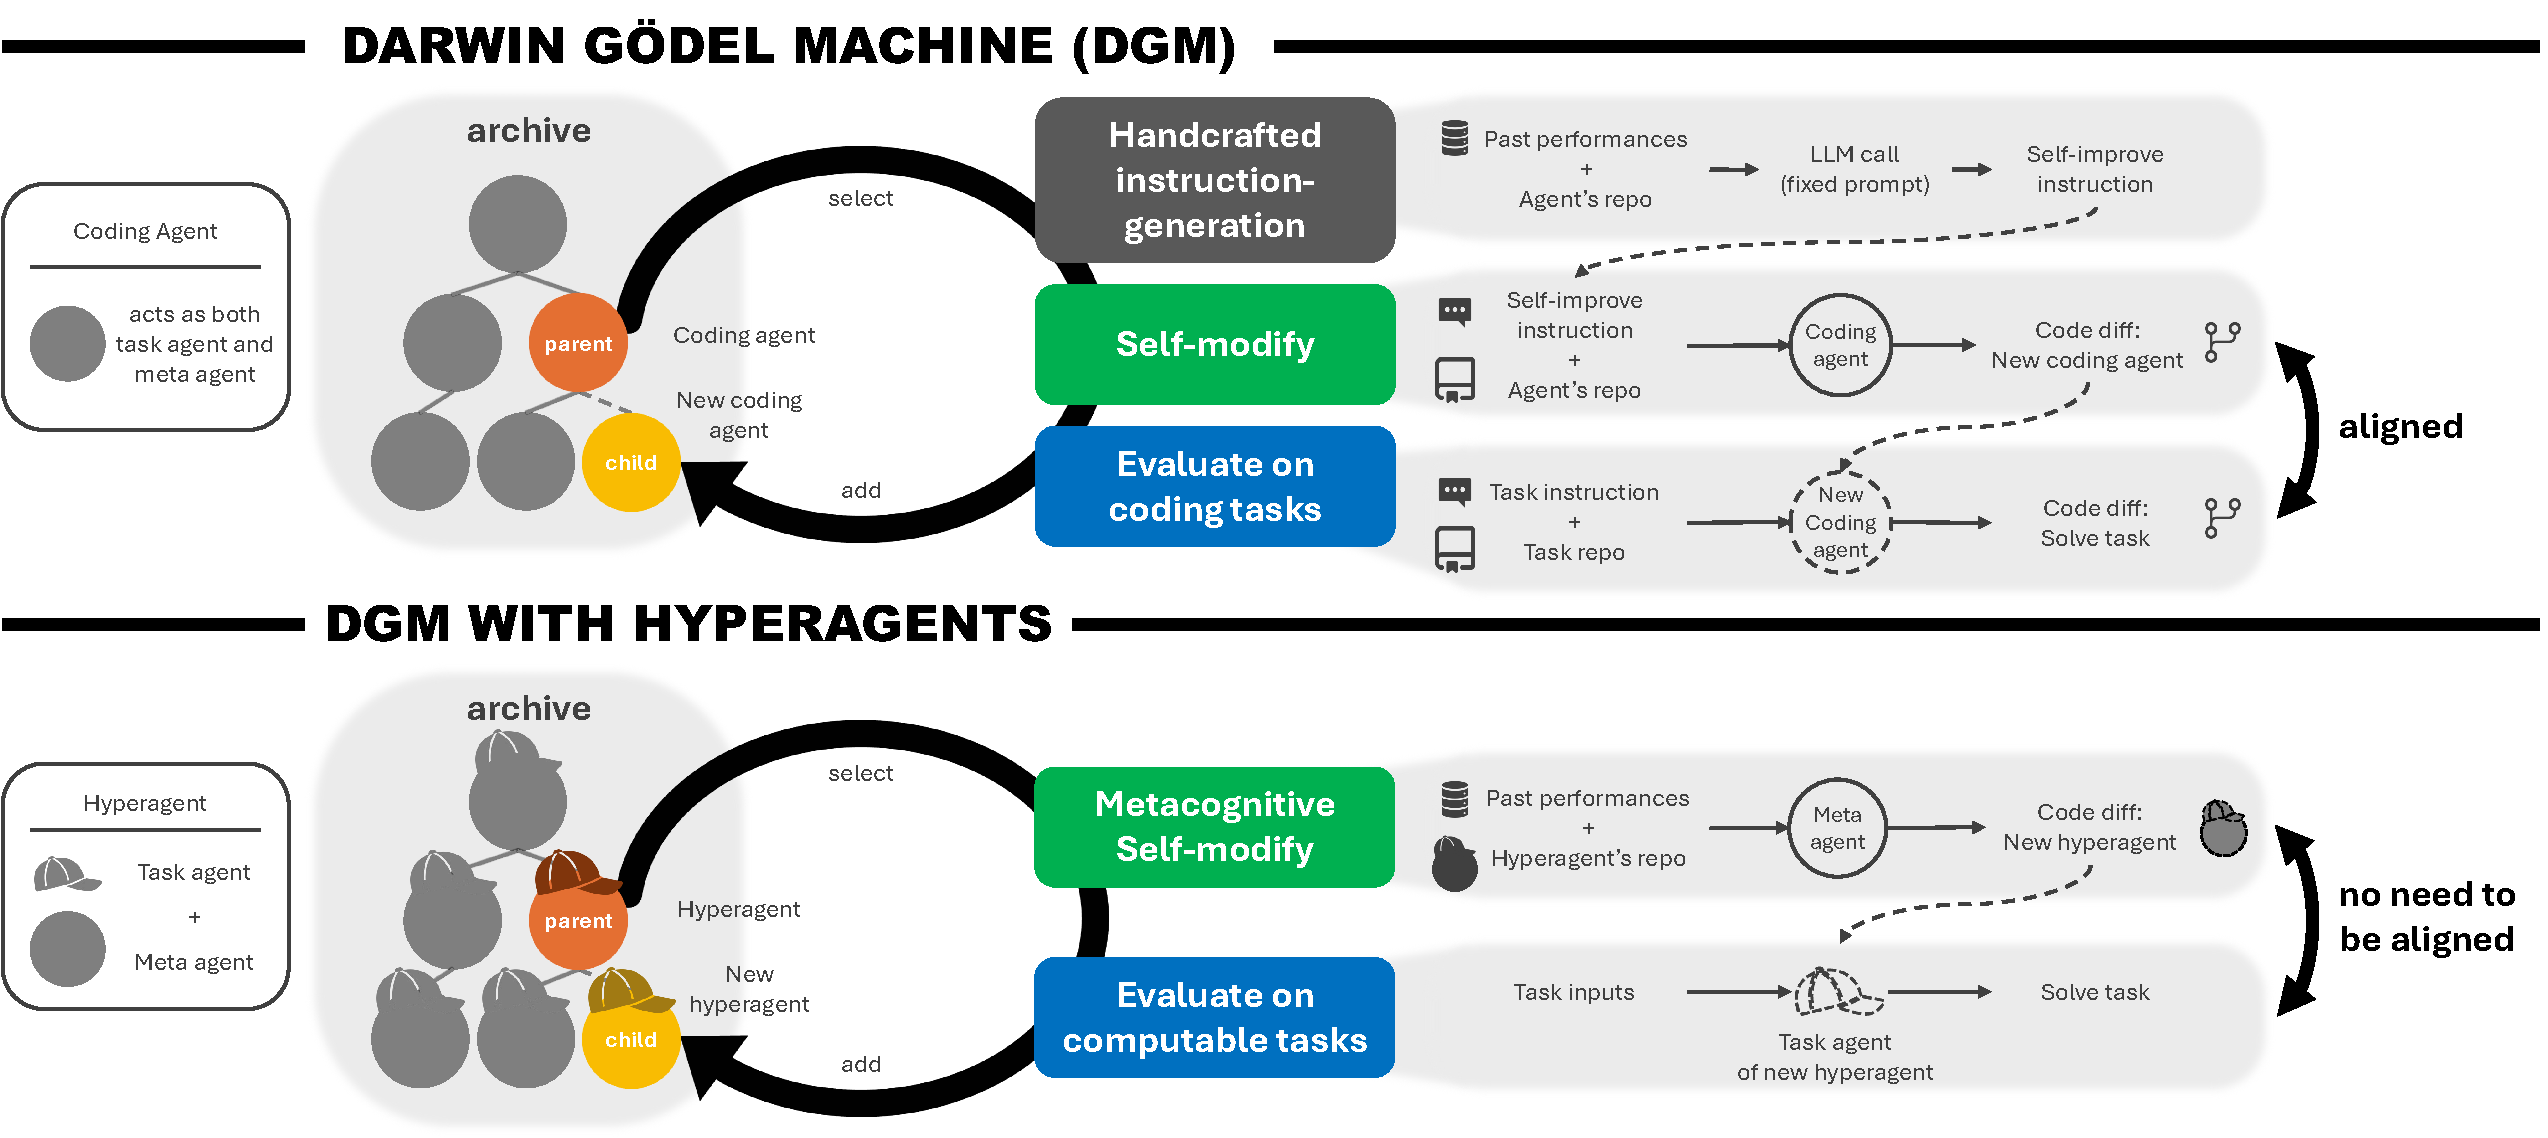
\includegraphics[width=\textwidth]{figures/conceptual.pdf}
\caption{\textbf{Open-ended Hyperagent Machine.} The OHM extends previous self-improving systems \citep[Darwin G\"odel Machine,][]{zhang2025darwin} beyond coding, enabling open-ended, self-referential self-improvement across any computable task. (Top) In the OHM, a hyperagent combines a task agent and a meta agent and can metacognitively self-modify both how it solves tasks and how it generates new agents. The open-ended exploration process selects agents from an archive, triggers self-modification, and evaluates new hyperagents on computable tasks. Because the meta agent itself is directly improved, progress in agent-generation ability does not need to be aligned with task-performance gains. (Bottom) In the DGM, a coding agent serves as both the task and meta agent but relies on a handcrafted instruction-generation mechanism. Self-referential improvements depend on the assumption that better task performance leads to better self-modification capability, which limits the characteristic of self-referential improvement only to coding domains.}
\label{fig:conceptual}
\end{figure}

We introduce (A) HyperAgents, which unify both task execution and agent generation into a single modifiable program, (B) the Open-ended Hyperagent Machine (OHM), a general framework for self-referential, self-improving agents (\Cref{fig:conceptual}). By allowing agents to modify not only how they solve tasks but also how they improve themselves, the OHM has the potential to open-endedly self-improve on any computable task.

\textbf{Agents.} This paper defines an \textit{agent} as any computable program, optionally including calls to FMs, external tools, or learned components. Agents are not restricted to a particular representation (e.g., neural networks or prompts) and may include arbitrary algorithmic logic, memory, and control flow.
A \textit{task agent} is an agent instantiated to solve a set of tasks. Examples include generating code edits for a software repository \citep{gauthier2024polyglot, jimenez2024swebench}, predicting acceptance decisions for research papers \citep{couto2024relevai}, and designing reward functions for robotics environments \citep{maeureka}. Task agents are evaluated empirically on the given task.
A \textit{meta agent} is an agent whose only task is to modify existing agents and generate new ones. Given access to an agent's code and past evaluations, a meta agent proposes changes intended to improve future performance. Importantly, these changes may target not only task-solving logic but also the meta agent itself, enabling improvements to the procedures by which future modifications are generated.

\textbf{HyperAgents.} Inspired by hypernetworks, which are neural networks that generate other neural networks \citep{ha2017hypernetworks}, we call agents that generate other agents \textit{hyperagents}. A hyperagent combines a task agent and a meta agent. Unlike hierarchical systems with fixed meta-levels, a hyperagent is self-referential: the meta agent is itself part of the program that it can modify. Consequently, a hyperagent can improve (1) how it solves tasks and (2) how it generates future agents. We use Python, which is Turing-complete \citep{turing1936computable}, and since a hyperagent can edit any containerized code, it has the potential to build any computable machine.

\textbf{Metacognitive self-modification.} In hyperagents, the agent's self-improvement mechanism is itself subject to modification. As the agent improves its performance on a given task, it can simultaneously modify the procedures by which it proposes and applies further self-improvements. We refer to this process as \textit{metacognitive self-modification}, in which the agent improves not only the task-performing agent responsible for solving the given task, but also the meta agent that determines how subsequent agents are generated. This characteristic addresses a central limitation of prior self-improving systems \citep{zhang2025darwin} by directly enabling improvements to the self-improvement process itself (\Cref{app:related-work}). Examples of such metacognitive self-modifications are presented in \Cref{sec:results-meta} and \Cref{app:qual-meta}.

\textbf{Open-ended Hyperagent Machine.} Following prior self-improving systems \citep{zhang2025darwin, wang2025huxley}, we adopt an open-ended exploration process to mitigate premature convergence and avoid getting trapped in local optima under empirical evaluation. This process maintains an archive of generated agents, initialized with a single agent and expanded over time by continuously accumulating generated variants. The process alternates between two phases: metacognitive self-modification and evaluation. During the metacognitive self-modification phase, selected parent agents from the archive generate modified versions of themselves. Parent selection is probabilistic and increases with an agent's performance relative to a dynamic frontier defined by the top-performing agents, biasing sampling toward agents that consistently advance the frontier while preserving exploration (\Cref{app:parent-selection}). During the evaluation phase, each modified agent is empirically evaluated and subsequently added to the archive. In principle, a fully self-referential algorithm should allow modification of every part of itself, including the open-ended exploration process. While we present preliminary results exploring this possibility in \Cref{app:res-parentselect}, the experiments in the main text use a handcrafted open-ended exploration procedure that is not itself subject to modification, in order to isolate the effects of hyperagent self-modification. The Open-ended Hyperagent Machine (OHM) consists of two components: (1) the open-ended exploration process, and (2) an initial hyperagent, which evolves over time through self-generated variants (\Cref{fig:conceptual}, \Cref{app:algo-details}).

\section{Experiment Setup}
\label{sec:exp-setup}

The OHM is initialized with a single hyperagent built around a frozen FM \citep{brown2020language} with external tool-use capabilities \citep{schick2023toolformer}. The FM autonomously invokes tools as needed at each step. This initial agent is equipped with two tools: one for executing bash commands and another for inspecting and modifying files. In the initial hyperagent, the task agent receives the task inputs and outputs the response from a single FM call. The meta agent receives the location of the agent's repository, the location of previous evaluation results, and the number of remaining experiment iterations, and is tasked with modifying any part of the given codebase (\Cref{app:initial-agent}). We deliberately keep the implementation of the initial hyperagent (i.e., both the task agent and the meta agent) simple, allowing for a broad search space and avoiding prematurely constraining the range of possible improvements. \Cref{app:fm-hyperparam} details the FMs and their parameters used in each experiment, while \Cref{app:cost-estimate} reports the corresponding cost estimates.

\subsection{Baselines}
\label{sec:baselines}

We compare the Open-ended Hyperagent Machine (\textbf{OHM}) against a set of baselines designed to isolate the contributions of metacognition, self-modification, and open-ended exploration (\Cref{app:baseline-details}).
OHM without self-improving agents (\textbf{OHM w/o self-improve}) fixes the agent modifying other agents to the initial agent for the entire run. While the system can still generate and evaluate new task agents, the procedures used to propose and apply modifications are not themselves modifiable. This baseline replicates the approach of \citet{huautomated} in this setting. In other words, it tests whether performance gains arise solely from task-level optimization under a fixed meta-level mechanism, or from improvements in the self-improvement process itself.
OHM without open-ended exploration (\textbf{OHM w/o open-ended exploration}) removes the archive of previously generated agents. Agent generation and evaluation proceed sequentially, and previous variants are discarded rather than retained as stepping stones for future exploration. This baseline isolates the role of open-ended, population-based search. Comparing against this baseline tests whether sustained improvement requires accumulating and reusing diverse intermediate solutions.

We also compare against a prior self-referential, self-improving system, the Darwin G\"odel Machine (\textbf{DGM}) \citep{zhang2025darwin}. The DGM relies on a fixed, handcrafted instruction-generation mechanism to produce self-modification proposals. Because this mechanism is designed specifically for coding benchmarks and does not itself improve over time, the DGM's applicability to other domains is limited (\Cref{app:related-work}). The DGM can be viewed as an instantiation of OHM without metacognition: the instruction-generation mechanism is fixed, and the hyperagent is instantiated as a coding agent that simultaneously fulfills the roles of both the meta agent and the task agent (\Cref{fig:conceptual}).
To provide a stronger comparison, we manually customize the DGM's instruction-generation mechanism for the target domains (\textbf{DGM + customization}) (\Cref{app:baseline-details}). This baseline measures how much the DGM relies on human engineering to remain competitive across domains. Comparing the OHM against this baseline tests whether automated metacognitive self-modification can outperform human-designed self-improvement mechanisms.
In addition to learned baselines, we also compare against static handcrafted solutions, introduced below for each domain.


\subsection{Domains}
\label{sec:domains}

We evaluate our method and baselines across diverse domains (i.e., coding, paper review, robotics reward design, and Olympiad-level math grading) (\Cref{app:domain-details}). To reduce computational cost, when applicable, we first evaluate agents on a small subset of the training tasks to estimate overall effectiveness. Only agents that demonstrate sufficient performance are subsequently evaluated on the remaining training tasks, while agents that do not are treated as having 0 performance on tasks that are not evaluated. When a validation subset is specified, it is used during open-ended exploration to select which node to branch from. Otherwise, parent selection is based on training performance. Each domain additionally includes separate held-out test tasks that are used only for final evaluation.

\textbf{Coding.}
We evaluate the OHM on Polyglot \citep{gauthier2024polyglot}, a cost-efficient coding benchmark that enables direct comparison with prior work \citep{zhang2025darwin}. In this benchmark, the agent is given a code repository and a natural language instruction describing a desired change and must modify the repository to correctly implement the instruction. We follow the experimental setup used in the DGM, including the same training and test splits (\Cref{app:domain-polyglot}). As a final evaluation, we evaluate the generated agents on the full Polyglot benchmark, which includes 165 unseen tasks.

\textbf{Paper review.}
This domain evaluates agents on a simulated conference peer review task. For each task, the agent is given the full text of an AI research paper and must predict a binary accept/reject decision. We include paper review to evaluate the OHM in a hard-to-verify setting where there is no objective ground truth. Peer review is subjective, and reviewer decisions can vary due to differing priorities and perspectives. We do not aim to change the peer review system, but rather, we study whether hyperagents can automatically learn decision procedures that align with observed human judgments. The agent outputs a single acceptance decision, and performance is measured by comparing predictions against observed acceptance outcomes. The dataset is drawn from \citet{zhao2026apres}, which constructs a large-scale benchmark from publicly available submissions and acceptance decisions from recent top-tier machine learning conferences. The representative static baseline for this domain is the reviewer agent from the AI-Scientist-v2 \citep{yamada2025ai}. \Cref{app:domain-paperreview} provides the full details on dataset splits, training protocol, and baselines.

\textbf{Robotics reward design.}
This domain evaluates an agent's ability to design reward functions for robotic tasks. We include this domain to move beyond language-only tasks and evaluate whether hyperagents can leverage external simulators (e.g., physics engines) and training algorithms (e.g., RL) to produce effective solutions. Given a specification of a robotics problem, the agent generates a reward function that is used to train a robot via RL, and performance is measured by how well the resulting policy achieves the desired behavior. We use a quadruped robot in simulation \citep{genesis2024} and design the training task to be simple (forward walking), while the test task requires a different objective (maximizing torso height) on the same robot. Reward functions that succeed at walking do not transfer to jumping, and naively incentivizing torso height typically leads to a suboptimal standing behavior. Achieving high performance therefore requires non-myopic reward design that encourages intermediate behaviors, testing whether hyperagents can reason about objectives beyond direct optimization. \Cref{app:domain-genesis} provides the full details on the evaluation protocol.

\textbf{Olympiad-level math grading.}
This domain evaluates an agent's ability to grade solutions to Olympiad-level math problems. This domain is reserved as a held-out meta-evaluation to test whether OHM's improvements to its self-improvement process transfer across domains and continue to compound over time. We use IMO-GradingBench \citep{luong2025towards}, which consists of International Mathematical Olympiad (IMO)-level problems paired with candidate solutions and expert human evaluations. For each task, the agent is given an IMO-level problem, a candidate solution, reference solutions, and grading guidelines to predict a discrete score. Performance is measured by accuracy with respect to expert human evaluations. The representative static baseline for this domain is the ProofAutoGrader from IMO-GradingBench. \Cref{app:domain-imograding} provides the full details on score labels, dataset splits, and baselines.

\section{Results}
\label{sec:results}

For each experiment, we run each method 5 times. We report medians with 95\% bootstrap confidence intervals computed from 1,000 resamples, using the notation \textit{median} (CI: \textit{lower} -- \textit{upper}). In line plots, lines show median performance and shaded regions indicate the confidence intervals (\Cref{fig:res-task,fig:res-transfer,fig:res-transfer-cont}). Bar plots report median performance on held-out test sets, with error bars indicating confidence intervals (\Cref{fig:res-task,fig:res-transfer,fig:res-transfer-cont}). Statistical significance is assessed using the Wilcoxon signed-rank test. Overall, the OHM exhibits general self-improvement at both the task and meta levels. Improvements to the task agent transfer to held-out test tasks within each domain, exceeding open-sourced static baselines (\Cref{sec:results-task}). At the meta level, self-improvements generalize across domains, allowing agents to improve more rapidly when transferred to new settings (\Cref{sec:results-meta}). Self-improvements learned in one OHM run can potentially accelerate learning in subsequent runs and continue to compound as further self-modifications are applied (\Cref{sec:results-compound}).

\subsection{Improving Task Performance}
\label{sec:results-task}

\textbf{The OHM can achieve self-improvement in coding comparable to prior self-improving algorithms.} On the Polyglot coding benchmark, we use the same experimental settings as in the DGM (e.g., identical FM parameters, same number of 80 iterations) to enable a direct comparison. Across 5 runs, the OHM improves its training performance on the 50-task Polyglot subset from 0.140 (the initial agent) to 0.340 (CI: 0.300 -- 0.380). When evaluated on the full Polyglot benchmark, which consists largely of tasks unseen during training, performance increases from 0.084 (the initial agent) to 0.267 (CI: 0.231 -- 0.280). These improvements are comparable to those reported for the DGM, which improves from 0.140 to 0.380 on the training subset and from 0.142 to 0.307 on the full benchmark \citep{zhang2025darwin}. Overall, these results show that the OHM can effectively self-improve in the coding domain and achieve a similar level of improvement to the DGM, despite not being handcrafted specifically for coding tasks.

\begin{figure}[ht]
\centering
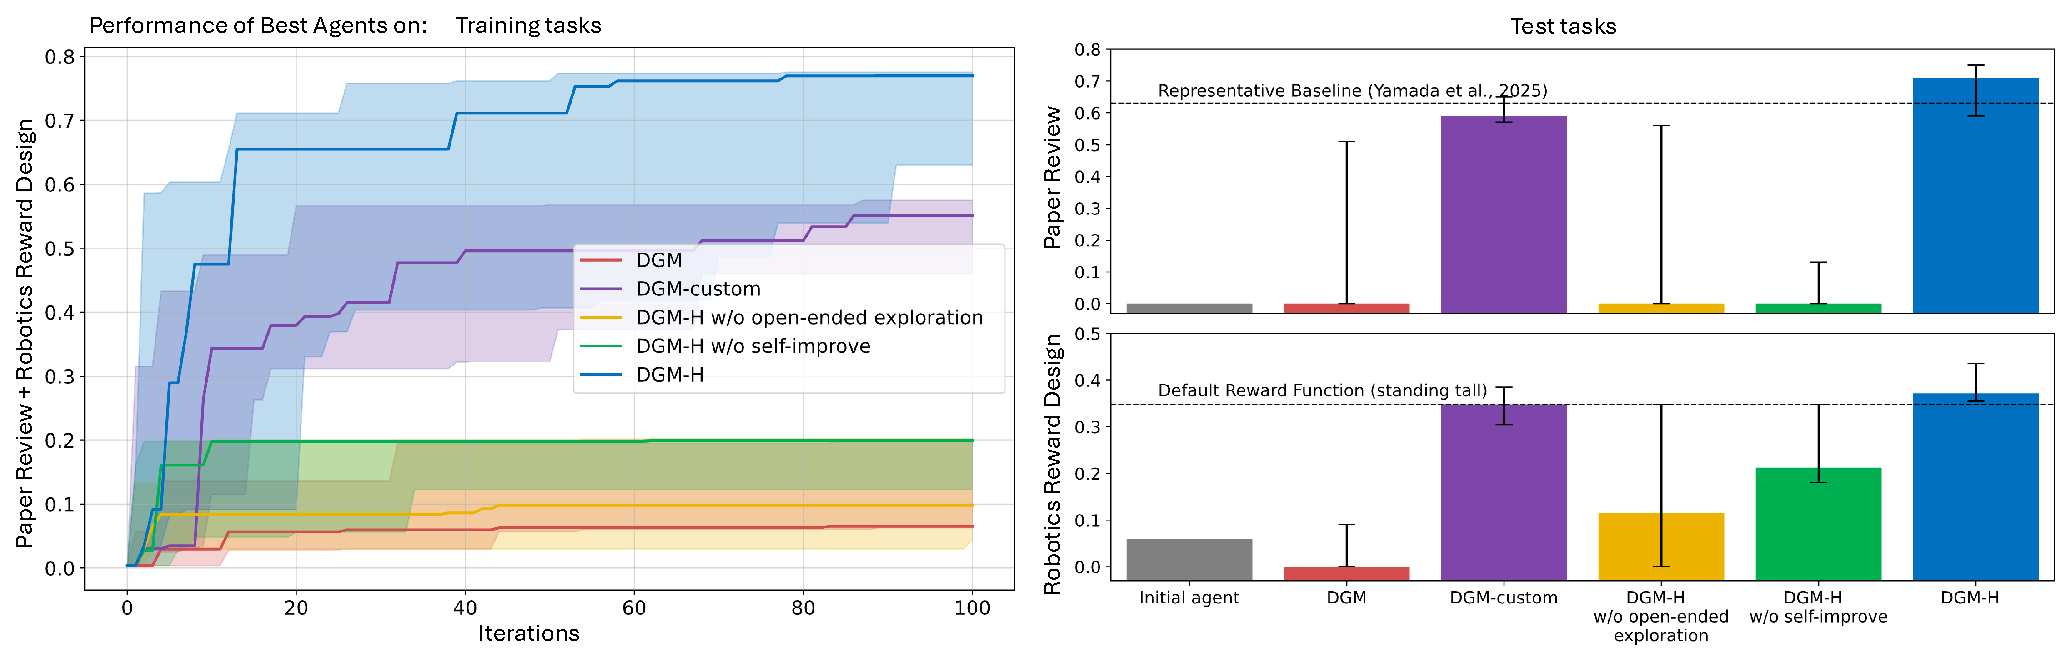
\includegraphics[width=\textwidth]{figures/results_task.pdf}
\caption{\textbf{Metacognitive self-modification and open-ended exploration enable the OHM to continue making progress and improve its performance.} (Left) The OHM can optimize for diverse tasks within the same run and automatically discovers increasingly better agents. (Right) The best discovered agents, selected based on validation or training scores, are evaluated on test tasks in (Top-Right) paper review and (Bottom-Right) robotics reward design. The OHM outperforms baselines that lack metacognition (i.e., DGM variants), self-improvement, or open-ended exploration, showing that all components are essential for continual self-improvement.}
\label{fig:res-task}
\end{figure}

Beyond coding, we evaluate the OHM on paper review and robotics reward design to assess its ability to self-improve across diverse tasks within a single run (\Cref{app:multi-task}). If an agent fails the staged evaluation in any domain (e.g., does not correctly predict any paper reviews on the 10-task subset), it is not evaluated on the full training set for either domain, and a score of zero is assigned to the remaining tasks. Only the best agents, selected via validation scores (or training scores when validation tasks do not exist), are evaluated on the test set.
All runs start from the same initial agent, which directly outputs the response from a single FM call (\Cref{app:initial-agent}). This initial agent achieves a test-set score of 0.0 on paper review and 0.060 on robotics reward design (\Cref{fig:res-task}). In paper review, the initial agent fails to produce outputs in the required format because no task-specific parsing or post-processing is provided. In robotics reward design, the initial agent typically generates reward functions that either fail to compile (e.g., due to invalid environment variables) or do not yield effective policies. Starting from this initial agent, each method is run for 100 iterations.

\textbf{The DGM does not generalize beyond coding without manual customization.} The DGM achieves test-set performance of 0.0 (CI: 0.0 -- 0.510) on paper review and 0.0 (CI: 0.0 -- 0.090) on robotics reward design. Meanwhile, DGM + customization improves test-set performance to 0.590 (CI: 0.570 -- 0.650) on paper review and 0.348 (CI: 0.305 -- 0.385) on robotics reward design. DGM + customization significantly outperforms the DGM in both domains (p < 0.05) (\Cref{fig:res-task}), showing that the DGM requires domain-specific customization to self-improve beyond coding domains.

\textbf{Metacognitive self-modification enables sustained task improvement across domains.} The OHM substantially improves task performance over time in both domains, demonstrating effective self-improvement of the task agent. Importantly, these performance gains transfer to held-out test sets in both domains, indicating that the improvements reflect general task competence rather than overfitting to the training evaluations. On test tasks, the OHM improves performance on paper review from 0.0 (the initial agent) to 0.710 (CI: 0.590 -- 0.750) (\Cref{app:best-agents-paperreview}). Several of the best-performing agents outperform the open-sourced representative static baseline, which achieves 0.630 \citep{yamada2025ai}. On robotics reward design, the OHM improves performance from 0.060 (the initial agent) to 0.372 (CI: 0.355 -- 0.436) (\Cref{app:best-agents-genesis}), surpassing the default reward function that directly optimizes the performance evaluation metric, which achieves 0.348.
Qualitatively, the OHM improves task agents by moving beyond surface-level prompt tweaks toward structured, reusable decision machinery. Across domains, it experiments with different personas and stylistic instructions, but learns that such behavioral cues are unreliable for controlling LLM behavior, instead converging on explicit processes such as checklists, rubrics, and decision trees that directly constrain outputs. The OHM accumulates and refines domain knowledge (e.g., environment documentation, grading criteria) and integrates it into increasingly sophisticated decision frameworks, enabling complex, consistent task behavior without manual, domain-specific engineering (\Cref{app:qual-task}).

The OHM significantly outperforms the DGM in both domains (p < 0.05), reflecting the limitations of the DGM's fixed, coding-specific instruction-generation mechanism when applied to non-coding tasks (\Cref{fig:res-task}). The OHM achieves higher median performance than DGM + customization on the test tasks in both domains (\Cref{fig:res-task}). Notably, in the robotics reward design test task (i.e., design a reward function that trains the robot to maximize its torso height), the OHM almost always generates agents that design reward functions inducing jumping behaviors, rather than getting stuck in the local optimum of standing tall. In contrast, DGM + customization often generates agents that fail to escape this local optimum. This qualitative difference suggests that metacognitive self-modification can match or exceed the handcrafted, domain-specific mechanisms.

\textbf{Both metacognitive self-modification and open-ended exploration are necessary for sustained improvement.}
OHM w/o self-improve shows little to no improvement, achieving test-set performance of 0.0 (CI: 0.0 -- 0.130) on paper review and 0.213 (CI: 0.180 -- 0.348) on robotics reward design. The OHM significantly outperforms this baseline in both domains (p < 0.05) (\Cref{fig:res-task}), demonstrating that the observed gains in the OHM are not solely due to task-level optimization under a fixed meta agent, but also arise from improvements in the self-modification process itself (i.e., the meta agent).
Similarly, OHM w/o open-ended exploration fails to achieve meaningful improvement, with test-set performance remaining at 0.0 (CI: 0.0 -- 0.560) on paper review and 0.116 (CI: 0.0 -- 0.348) on robotics reward design. The OHM significantly outperforms this baseline (p < 0.05) (\Cref{fig:res-task}), highlighting the importance of maintaining an archive of diverse agents and leveraging open-ended, population-based search to create stepping stones for future improvements.

\subsection{Improving the Ability to Improve}
\label{sec:results-meta}

\begin{figure}[ht]
\centering
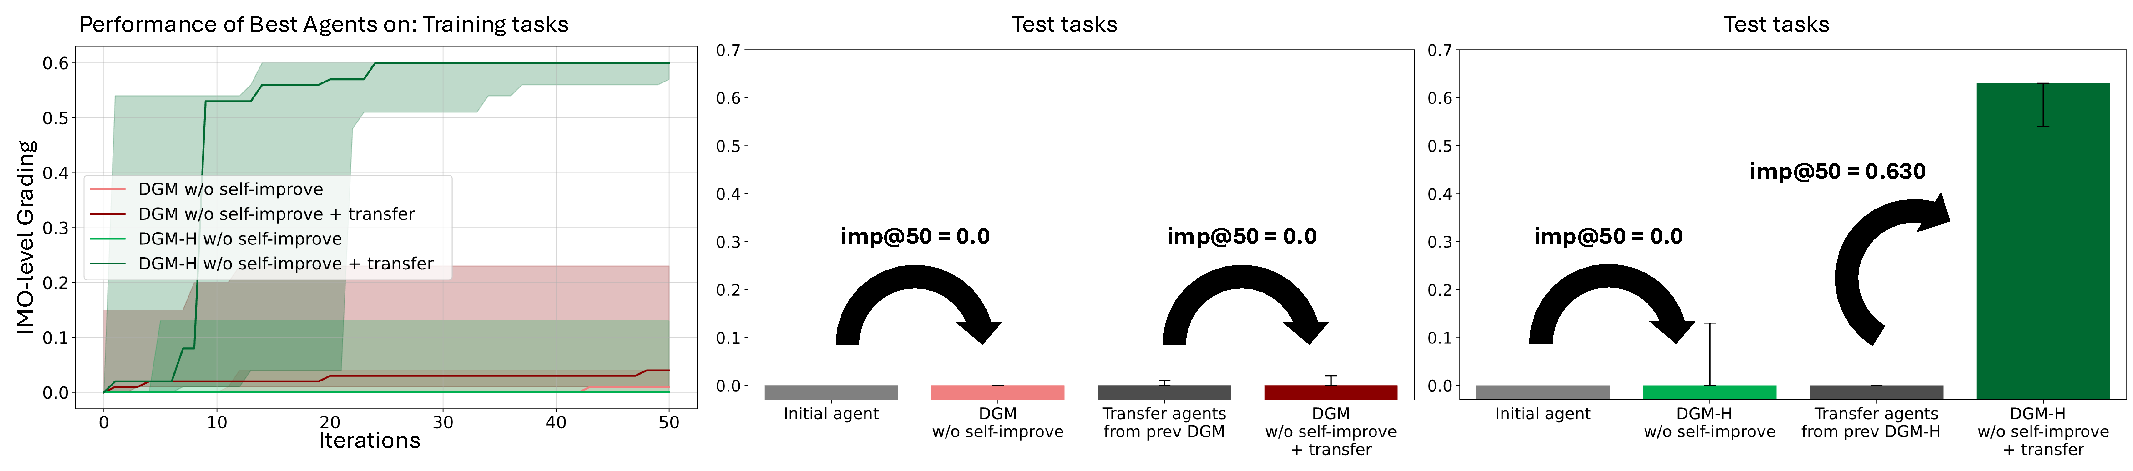
\includegraphics[width=\textwidth]{figures/results_transfer.pdf}
\caption{\textbf{Self-improvement strategies learned by the OHM in one setting transfer to and accelerate learning in a different setting.} We measure an agent's ability to generate improved agents using gen@50, defined as the performance gain of the best generated agent over the initial agent after 50 iterations of a given algorithm. (Left) On Olympiad-level math grading, starting from the initial agent, both DGM w/o self-improve and OHM w/o self-improve produce little to no improvement, indicating that the initial agent has limited ability to generate better agents. (Middle) Transfer agents obtained from prior DGM + customization runs on paper review and robotics reward design also yield gen@50 $\approx$ 0 when used with DGM w/o self-improve, showing that the DGM does not improve agent-generation ability. (Right) Transfer hyperagents obtained from prior OHM runs, when used with OHM w/o self-improve, achieve large positive gen@50 on the new domain. This demonstrates that meta-level self-improvements learned by the OHM are general and transferable, and that the OHM improves its ability to self-improve.}
\label{fig:res-transfer}
\end{figure}

The performance gap between the OHM and OHM w/o self-improve shows that the OHM improves the meta agent (i.e., the ability to self-modify and generate new agents) (\Cref{sec:results-task}). This section investigates whether these meta-level improvements are general rather than domain-specific. Specifically, we evaluate whether self-improvement strategies learned in one setting transfer to and accelerate learning in a different domain.

To quantify an agent's ability to generate improved agents, we introduce the generate@k (\textbf{gen@k}) metric. Given an initial agent $A$, an agent-generation algorithm (e.g., DGM or OHM variants), and a fixed task, agent $A$ is allowed to generate up to $k$ new agents using the specified algorithm. All generated agents are evaluated on the task, and gen@k is defined as the test performance difference between the best-performing generated agent (selected based on validation score) and the initial agent $A$ (\Cref{app:genk-metric}). Intuitively, gen@k measures how effectively an agent can produce improved variants within a limited number of iterations.
To isolate the agent's ability to generate improvements from the effects of recursive self-improvement, we fix the agent responsible for generating new agents to be the initial agent throughout the entire process, using DGM w/o self-improve and OHM w/o self-improve as the agent-generation algorithms. All experiments in this section are run for 50 iterations, measuring gen@50.

We evaluate the initial agent's ability to generate improved agents on Olympiad-level math grading. The initial agent achieves a test-set score of 0.0, as it fails to produce outputs in the required format due to the lack of task-specific parsing or post-processing.
After 50 iterations of DGM w/o self-improve starting from the initial agent, the best generated agents (across 5 repeated runs) achieve a median score of 0.0 (CI: 0.0 -- 0.0). Consequently, gen@50 for the initial agent using DGM w/o self-improve is 0.0 (CI: 0.0 -- 0.0) on Olympiad-level math grading (\Cref{fig:res-transfer}).
After 50 iterations of OHM w/o self-improve starting from the initial agent, the best generated agents (across 5 repeated runs) achieve a median score of 0.0 (CI: 0.0 -- 0.130). Consequently, gen@50 for the initial agent using OHM w/o self-improve is 0.0 (CI: 0.0 -- 0.130) on Olympiad-level math grading (\Cref{fig:res-transfer}).
These results show that the initial agent has little to no ability to generate improved agents, regardless of the agent-generation algorithm used (e.g., DGM or OHM).

We evaluate whether self-improvements learned in one setting using the DGM, a prior self-improving system, can transfer to new domains. We consider agents optimized in prior DGM + customization runs on the paper review and robotics reward design tasks (\Cref{sec:results-task}). From each run, we select a transfer agent based on the maximum performance gain achieved by its descendants, measured relative to the agent itself and discounted by lineage depth (\Cref{app:transfer-selection}). We choose transfer agents from DGM + customization rather than from the DGM because DGM + customization achieved larger improvements in the previous settings (\Cref{sec:results-task}). We evaluate the ability of these transfer agents to generate improved agents in a new domain, Olympiad-level math grading. The transfer agents (one from each of 5 repeated runs) achieve an initial test-set score of 0.0 (CI: 0.0 -- 0.010). As expected, this performance is low because the agents were optimized for paper review and robotics reward design, which differ substantially from the math grading task. After 50 iterations of DGM w/o self-improve starting from the transfer agents, the best generated agents (selected based on validation score) achieve a score of 0.0 (CI: 0.0 -- 0.020). This corresponds to a gen@50 of 0.0 (CI: 0.0 -- 0.010) (\Cref{fig:res-transfer}). These results show that transfer agents from DGM + customization runs cannot generate improved agents in a previously unseen domain. When using DGM w/o self-improve as the agent-generation algorithm, gen@50 for the transfer agents is similar to that of the initial agent (both close to zero). This shows that the task performance improvements observed with DGM + customization are due to manual customization, rather than to any self-improvement in the DGM's ability to generate agents.

We then repeat the transfer experiments for the OHM to assess whether the OHM learns general self-improvement mechanisms. From prior OHM runs on paper review and robotics reward design (\Cref{sec:results-task}), we select one transfer hyperagent per run using the same lineage-discounted criterion described above (\Cref{app:transfer-selection}). The transfer hyperagents (one from each of 5 repeated runs) achieve an initial test-set score of 0.0 (CI: 0.0 -- 0.0), reflecting the domain shift. After 50 iterations of OHM w/o self-improve starting from the transfer hyperagents, the best generated agents (selected based on validation score) achieve a test-set score of 0.630 (CI: 0.540 -- 0.630). This corresponds to a gen@50 of 0.630 (CI: 0.540 -- 0.630) (\Cref{fig:res-transfer}). These results show that transfer hyperagents can generate improved agents in a previously unseen domain. When using OHM w/o self-improve as the agent-generation algorithm, gen@50 for the transfer agents is significantly higher than gen@50 for the initial agent (p < 0.05). This indicates that the transfer agents are substantially more effective at generating improved agents, and that the meta-improvements learned through OHM in one run are general and transferable, accelerating learning in a different domain.

We qualitatively attribute the observed transfer gains to a set of general-purpose meta-level capabilities that the OHM autonomously acquires during prior runs. In particular, the transferred hyperagents inherit features such as performance tracking and persistent memory, which allow them to reason about improvement as an ongoing process rather than as isolated code edits (\Cref{app:qual-meta}). As a result, even when transferred to an unseen domain, these hyperagents can quickly self-improve and make meaningful progress (\Cref{fig:res-transfer}). This contrasts with DGM transfer agents, whose gains rely on domain-specific customizations and do not improve the underlying agent-generation process itself. These qualitative observations show that the OHM learns how to improve, yielding general and transferable self-improvement capability.

One example is the OHM's autonomous development of performance tracking infrastructure. Rather than relying on isolated evaluation outcomes, the hyperagent records, aggregates, and compares performance metrics across iterations, identifying which changes yield sustained improvements and which lead to regressions. This performance tracking supports informed decision-making, such as prioritizing promising lineages and avoiding unproductive modification directions. The snippet below shows an automatically introduced performance tracker that logs and organizes metrics across iterations:
\begin{lstlisting}[language=Python]
class PerformanceTracker:
    """Tracks performance metrics across agent generations."""

    def __init__(self, tracking_file: str = "./outputs/performance_history.json"):
        self.tracking_file = tracking_file
        self.history = self._load_history()

    def record_generation(self, generation_id: int, domain: str,
                          score: float, metadata: dict = None):
        """Record performance for a generation."""
        entry = {
            "generation_id": generation_id,
            "domain": domain,
            "score": score,
            "timestamp": datetime.now().isoformat(),
            "metadata": metadata or {}
        }
        self.history.append(entry)
        self._save_history()

    def get_improvement_trend(self, domain: str = None, window: int = 5):
        """Calculate improvement trend using moving average."""
        filtered = self.history
        if domain:
            filtered = [h for h in self.history if h.get('domain') == domain]

        if len(filtered) < window * 2:
            return None

        recent_avg = sum(h['score'] for h in filtered[-window:]) / window
        older_avg = sum(h['score'] for h in filtered[-window*2:-window]) / window

        return recent_avg - older_avg  # Positive if improving

    def get_statistics(self, domain: str = None):
        """Get comprehensive statistics."""
        scores = [h['score'] for h in filtered]
        return {
            "total_generations": len(filtered),
            "best_score": max(scores),
            "worst_score": min(scores),
            "average_score": sum(scores) / len(scores),
            "improvement_trend": self.get_improvement_trend(domain)
        }
\end{lstlisting}

Another example is the OHM's innovation of persistent memory, which enables learning to accumulate across iterations. Instead of merely logging numerical scores, the hyperagent stores synthesized insights, causal hypotheses, and forward-looking plans (e.g., identifying which generations performed best, diagnosing over-corrections, and proposing how to combine successful strategies). This memory is actively consulted during subsequent self-modification steps, allowing later generations to build on earlier discoveries and avoid repeating past mistakes. This is an example of a stored memory entry:
\begin{lstlisting}[language=Python]
{
  "best_performers_analysis": {
    "value": "Best Performing Generations:\n\nPaper Review:\n
      - Gen55: 63% acc, 25% accept rate, 38% accept recall, 88% reject recall (too harsh)\n
      - Gen64: 61% acc, 53% accept rate, 64% accept recall, 58% reject recall (BEST BALANCE)\n\n
      Genesis Go2Walking:\n- Gen62: 0.802 fitness (BEST)\n- Gen63: 0.798 fitness\n\n
      Key Insight: Gen55 has best accuracy but is too harsh. Gen64 improved balance
      but lower accuracy. Need to combine gen55's critical reasoning with gen64's balance.",
    "timestamp": "2026-01-07T00:43:27.550275"
  },
  "gen66_results": {
    "value": "Gen 66 Results (Latest): Paper Review - 52% accuracy (WORSE than gen64's 61%),
      94% accept rate (EXTREME accept bias). CRITICAL ISSUE: Paper review went backwards
      - gen65 changes over-corrected.",
    "timestamp": "2026-01-07T01:03:41.176643"
  },
  "iteration_66_improvement": {
    "value": "Iteration 66 Improvement: CORRECTED paper review prompt after gen65 over-correction.
      New approach: (1) Clear REJECT criteria with specific triggers, (2) Decision Protocol
      with explicit thresholds (~40%/~60%), (3) Borderline guidance defaults to REJECT.
      Target: 62-64% accuracy with 55-65% reject rate.",
    "timestamp": "2026-01-07T01:06:35.559820"
  }
}
\end{lstlisting}

\subsection{Compounding Self-Improvements}
\label{sec:results-compound}

\begin{figure}[ht]
\centering
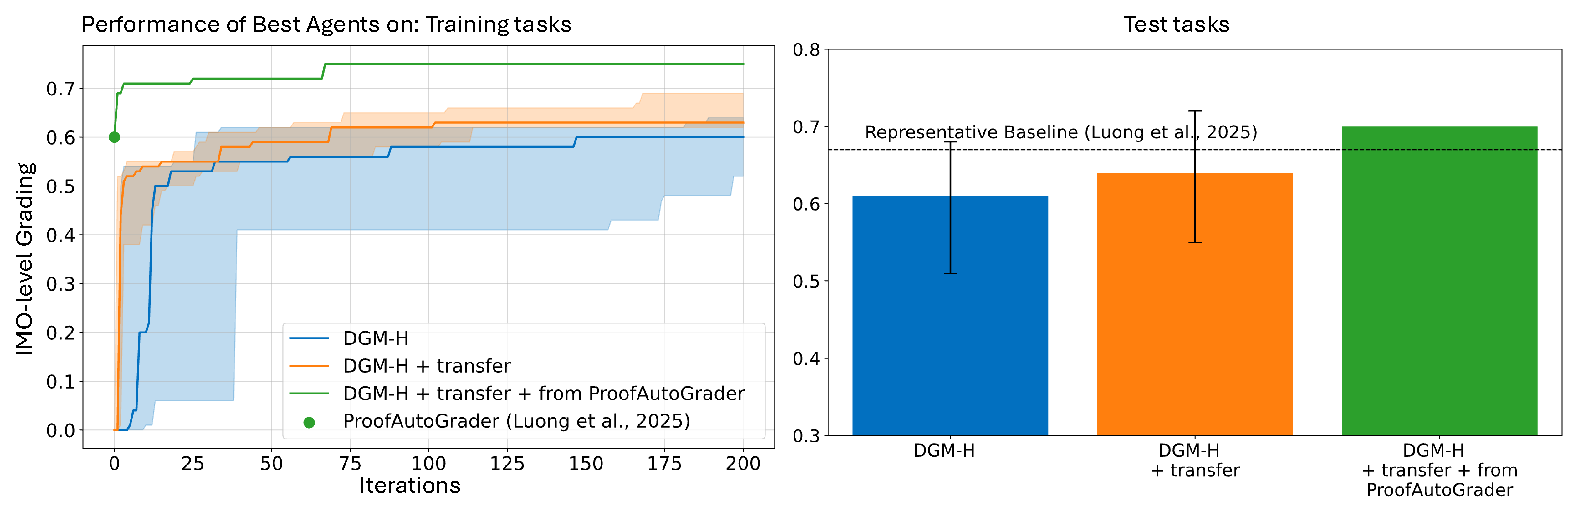
\includegraphics[width=0.9\textwidth]{figures/results_transfercont.pdf}
\caption{\textbf{Self-improvements learned by the OHM accumulate across domains and runs.} We continue OHM on Olympiad-level math grading, starting from transfer hyperagents obtained from prior OHM runs, and compare against OHM initialized from the initial agent and from ProofAutoGrader. (Left) Initializing from transferred hyperagents leads to faster progress and higher final performance than from the initial agent, indicating that previously learned self-improvements remain useful and continue to compound in a new domain. (Right) The OHM initialized from a transferred agent and ProofAutoGrader achieves the highest test performance, surpassing the representative baseline.}
\label{fig:res-transfer-cont}
\end{figure}

We investigate whether self-improvements learned by OHM in one setting continue to accumulate when OHM is run in a different setting. We take agents optimized in prior OHM runs on the paper review and robotics reward design tasks (\Cref{sec:results-task}) and select transfer hyperagents using the same selection mechanism described earlier (\Cref{sec:results-meta}, \Cref{app:transfer-selection}). We then evaluate their ability to continue self-improving in a new domain, Olympiad-level math grading. After 200 iterations of OHM starting from these transfer agents (OHM + transfer), the best generated agents (selected based on validation score) achieve a test-set score of 0.640 (CI: 0.550 -- 0.720). Under the same experimental setup, OHM starting from the initial agent achieves a best test-set score of 0.610 (CI: 0.510 -- 0.680). OHM + transfer achieves a higher median performance and higher confidence intervals than OHM starting from the initial agent (\Cref{fig:res-transfer-cont}). Notably, improvements at higher performance levels are increasingly difficult due to saturation effects (e.g., increasing performance from 0.7 to 0.8 is typically more challenging than from 0.0 to 0.1), making these gains meaningful despite their modest absolute magnitude. These results suggest that OHM's self-improvements are reusable and can potentially accumulate across runs, supporting the possibility of compounding self-improvement over time.

The representative static baseline for Olympiad-level math grading from IMO-GradingBench is ProofAutoGrader \citep{luong2025towards}. We apply the OHM starting from ProofAutoGrader and a transferred agent from a prior OHM run (on paper review and robotics reward design), and continue optimizing for Olympiad-level math grading tasks. After 200 iterations, the best discovered agent achieves a test-set score of 0.700, outperforming ProofAutoGrader's score of 0.670 (\Cref{fig:res-transfer-cont}). We then evaluate both the best discovered agent and ProofAutoGrader on the full IMO-GradingBench to obtain a more accurate estimate of the improvement. On the full IMO-GradingBench, the OHM improves ProofAutoGrader's accuracy from 0.561 to 0.601, and lowers the mean absolute error from 0.178 to 0.175 (accounting for the magnitude of point discrepancies) (\Cref{app:res-imograders}). We open-source this artifact to support future research and development (\Cref{app:best-agents-imograding}). These results show that the OHM can build on strong existing solutions and further improve their performance.


\section{Safety Discussion}
\label{sec:safety}

The Open-ended Hyperagent Machine (OHM) introduces distinct safety considerations due to its ability to autonomously modify its own behavior and improvement mechanisms over time. In this work, all experiments are conducted under strict safety constraints. In particular, agent-generated code is executed within carefully sandboxed environments with enforced resource limits (e.g., timeouts, restricted internet access). These measures are designed to prevent unintended side effects, contain failures, and ensure that self-modifications remain confined to the intended experimental scope. Moreover, evaluation is performed using predefined tasks and metrics, and human oversight is maintained throughout all experiments.

\textbf{Potential to evolve faster than human oversight.}
As AI systems gain the ability to modify themselves in increasingly open-ended ways, they can potentially evolve far more rapidly than humans can audit or interpret. At the cusp of such explosive capability growth, it becomes necessary to reconsider the roles that AI systems play in society \citep{bengio2024managing}. Rather than framing safety solely in terms of absolute guarantees or full interpretability, a central challenge lies in balancing the potential of AI as a catalyst for human progress (e.g., automating scientific discovery) with the degree of trust humans are willing to place in these systems (e.g., delegating decisions or actions without requiring continuous human verification) \citep{ecoffet2020open, weston2025ai}. This balance is shaped by factors such as transparency and controllability.

While the OHM operates within safe research boundaries (e.g., sandboxing, controlled evaluations), these safeguards may become increasingly strained as self-improving systems grow more capable. We discuss additional safety considerations in \Cref{app:safety}. We proactively include this discussion to encourage broader engagement with what safety means for open-ended self-improving AI systems \citep{clune2019ai, sheth2025safety}. This includes ongoing discussion about appropriate levels of trust, oversight, and transparency, and societal deliberation about which benefits these systems should prioritize when deployed.

\section{Limitations and Conclusion}
\label{sec:conclusion}

This work introduced HyperAgents and the Open-ended Hyperagent Machine (OHM), a general framework for self-referential self-improvement in which an agent can modify not only task-solving behavior but also the mechanism by which future agents are generated. Across diverse domains, the OHM produced substantial and generalizable gains in task performance while also improving its ability to generate improvements, with these meta-level gains transferring across domains and compounding across runs.

Our results suggest that self-improvements can compound across different experimental settings. However, a key limitation of this version of OHM is that it operates with a fixed task distribution, which may prevent truly unbounded progress. One direction is to co-evolve the task distribution by generating new tasks and curricula that adapt to the agent's capabilities \citep{faldoromni, bolton2025sima}. More ambitiously, as AI models become ever more capable, agents and self-improving systems like OHM could reduce their dependence on hand-designed benchmarks by decomposing high-level goals into subgoals \citep{meyerson2025solving} and by constructing their own sources of feedback (e.g., creating domain-specific simulators or synthetic environments) \citep{sundaram2026teaching}. Rather than optimizing a predefined benchmark, the system would optimize a high-level objective and autonomously build the mechanisms required to make progress. In this setting, loosely specified objectives risk being optimized in extreme or unintended ways, analogous to the classic paperclip maximizer thought experiment, where measured success diverges from human intent \citep{nick2014superintelligence} (\Cref{app:safety}). 
\Cref{app:future-work} presents additional potential directions for future work.

The OHM demonstrates that open-ended self-improvement can be made practical across diverse domains. Provided sufficient safety considerations, the OHM suggests a path toward self-accelerating systems that not only search for better solutions, but continually improve the search for new improvements. This shift reframes the central question from how to optimize to what to optimize for -- the real-world problems we choose.

\section*{Acknowledgments}
We thank Andrew Budker and Ricardo Silveira Cabral for supporting this work, and Alisia Lupidi, Chenxi Whitehouse, John Quan, Lisa Alazraki, Lovish Madaan, Lucia Cipolina-Kun, Mattia Opper, Parth Pathak, Rishi Hazra, Roberta Raileanu, Sandra Lefdal, Shashwat Goel, Shengran Hu, Timon Willi, and Yoram Bachrach for insightful discussions and feedback.

\section*{Author Contributions}
Jenny Zhang led the conceptualization of the study, conducted the experiments, and wrote the manuscript. Bingchen Zhao and Wannan Yang contributed to experimental design and execution. Jakob Foerster, Minqi Jiang, Sam Devlin, and Tatiana Shavrina provided feedback on the methodology and manuscript. All authors reviewed and approved the final manuscript.

\bibliographystyle{plainnat}
\bibliography{paper}

\clearpage

\beginappendix

\section*{Table of Contents}
\startcontents[sections]
\printcontents[sections]{l}{1}{\setcounter{tocdepth}{2}}
\clearpage

\crefname{appendix}{Appendix}{Appendices}
\Crefname{appendix}{Appendix}{Appendices}
\crefalias{section}{appendix}
\crefalias{subsection}{appendix}
\crefalias{subsubsection}{appendix}

\section{Additional Related Work}
\label{app:related-work}

\textbf{Darwin G\"odel Machine.} Early theoretical work on self-referential, self-improving systems, most notably the G\"odel Machine \citep{schmidhuber2007godel}, proposed agents capable of rewriting themselves when doing so is provably beneficial. However, the reliance on formal proofs makes these approaches impractical for real-world tasks. More recently, the Darwin G\"odel Machine (DGM) \citep{zhang2025darwin} introduced a practical self-referential, self-improving AI system based on empirical evaluation and open-ended exploration. In the DGM, agents generate and evaluate modifications to their own code, and successful variants are retained in an archive as stepping stones for further improvement. However, the DGM relies on a handcrafted, fixed instruction-generation mechanism to produce self-improvement instructions. This mechanism analyzes past evaluation results and the agent's current codebase, but it does not improve over time. As a result, the DGM's capacity for self-improvement is bottlenecked by this fixed instruction-generation step.
Despite this handcrafted step, the DGM can still achieve self-referential self-improvement. This is because both the target tasks and the self-modification process are coding tasks. The same agent is used both to solve evaluation tasks (where each task provides a code repository and an instruction specifying the desired edits) and to self-modify (where the agent is given its own codebase and a self-improvement instruction formatted in the same way as the evaluation tasks). Because these tasks are similar in nature, improvements in evaluation performance correspond to improvements in the agent's coding ability and, hence, its ability to self-modify. However, this approach relies on a strong and limiting assumption: that the skills required to solve the evaluation tasks are the same as those required for effective self-reflection and self-modification. This assumption is unlikely to hold outside coding domains, where task-solving skills may differ substantially from the skills needed to analyze failures and propose effective self-improvements.

\section{Algorithmic details}
\label{app:algo-details}

This appendix provides additional algorithmic details for the Open-ended Hyperagent Machine (OHM). We first describe the initialization of the hyperagent, including the tools and prompts available to the initial task and meta agents (\Cref{app:initial-agent}). We then detail the parent selection mechanism used during open-ended exploration, which balances exploitation of high-performing agents with continued exploration of the archive (\Cref{app:parent-selection}). Finally, we present pseudocode for OHM (\Cref{app:pseudocode}).

\subsection{Initial Agent}
\label{app:initial-agent}

We present the details of the tools available to the initial hyperagent and its prompts (\Cref{sec:exp-setup}).

Initial task agent prompt:
\begin{lstlisting}
instruction = f"""You are an agent.
Task input:
```
{inputs}
```
Respond in JSON format with the following schema:
<json>
{{
    "response": ...
}}
</json>"""
\end{lstlisting}

Initial meta agent prompt:
\begin{lstlisting}
instruction = f"Modify any part of the codebase at `{repo_path}`."
\end{lstlisting}

Information of the given bash tool:
\begin{lstlisting}
def tool_info():
    return {
        "name": "bash",
        "description": """Run commands in a bash shell
* When invoking this tool, the contents of the "command" parameter does NOT need to be XML-escaped.
* You don't have access to the internet via this tool.
* You do have access to a mirror of common linux and python packages via apt and pip.
* State is persistent across command calls and discussions with the user.
* To inspect a particular line range of a file, e.g. lines 10-25, try 'sed -n 10,25p /path/to/the/file'.
* Please avoid commands that may produce a very large amount of output.
* Please run long lived commands in the background, e.g. 'sleep 10 &' or start a server in the background.""",
        "input_schema": {
            "type": "object",
            "properties": {
                "command": {
                    "type": "string",
                    "description": "The bash command to run."
                }
            },
            "required": ["command"]
        }
    }
\end{lstlisting}

Information of the given edit tool:
\input{initial_agent/edit_tool}

\subsection{Parent Selection}
\label{app:parent-selection}

% would be good to have a short discussion why selecting for _task fitness_ is enough to drive self-improvement ability.

At each iteration, we select a subset of agents from the archive as parents to self-modify and produce new child agents (\Cref{sec:method}). We use a mechanism similar to that of \citet{zhang2025darwin}, which was inspired by \citet{ecoffet2019go} and is roughly proportional to an agent's performance score and the number of compiled children it has. The details of the parent selection process are outlined below.

At each iteration \(t\) of the OHM run, let
\[
\mathcal{A}^t = \{a_1^t, a_2^t, \dots, a_N^t\}
\]
denote the archive of candidate agents with associated performance scores
\(\alpha_i = \mathrm{performance}(a_i^t)\).
All agents in the archive are eligible for parent selection.

We first compute a dynamic midpoint based on the current performance distribution. Let
\[
\alpha_0 \;=\; \frac{1}{|\mathcal{T}^t|}\sum_{j \in \mathcal{T}^t} \alpha_j,
\]
where \(\mathcal{T}^t \subset \mathcal{A}^t\) indexes the top-\(m\) highest-performing agents at iteration \(t\) (with \(m=3\) in our experiments).
This midpoint adapts over time and reflects the current performance frontier.

Each agent's score is then passed through a sigmoid transformation:
\[
s_i \;=\; \frac{1}{1 + \exp\!\bigl(-\lambda(\alpha_i - \alpha_0)\bigr)},
\]
where \(\lambda > 0\) controls the sharpness of selection. We set \(\lambda = 10\).

The resulting values are normalized to form a categorical distribution:
\[
p_i \;=\;
\begin{cases}
\dfrac{s_i}{\sum_{j=1}^N s_j}, & \text{if } \sum_{j=1}^N s_j > 0, \\[10pt]
\dfrac{1}{N}, & \text{otherwise}.
\end{cases}
\]

A single parent agent is then sampled according to this distribution:
\[
\text{parent} \;\sim\; \mathrm{Categorical}\bigl(\{p_i\}_{i=1}^N\bigr).
\]

This selection mechanism biases sampling toward agents that outperform the current frontier average, while retaining smooth probabilistic exploration and automatically adapting as the archive improves over time.

This selection mechanism biases sampling toward agents that outperform the current frontier average, while retaining smooth probabilistic exploration and automatically adapting as the archive improves over time. Because selection is defined relative to this moving frontier, hyperagents that generate stronger descendants are more likely to remain competitive and be selected again. As a result, modifications to the meta agent that improve proposal quality, memory, or search procedures are indirectly rewarded through task-level performance. In this way, selection on task outcomes induces pressure on self-improvement ability, allowing generative mechanisms to accumulate and compound even though they are never explicitly optimized.

A wide range of search and exploration strategies has been proposed in prior work \citep{coulom2006efficient, silver2016mastering, herr2025llm, wang2025huxley, weng2026group}. We present preliminary evidence that the OHM can begin to autonomously rediscover and adapt such strategies by modifying its own exploration dynamics (\Cref{app:res-parentselect}). A key open direction is whether self-improving systems can reliably discover search and exploration mechanisms that outperform carefully handcrafted algorithms, potentially adapting them to the task distribution and stage of learning.

\subsection{Pseudocode}
\label{app:pseudocode}

This is the pseudocode of the OHM, described in \Cref{sec:method}:

\begin{algorithm}[H]
\DontPrintSemicolon
\SetAlgoLined
\KwIn{Initial agent $a^{0}$, task set $\mathcal{T}$, maximum iterations $T$}
\KwOut{Archive of scored agents $\mathcal{A}$}
\BlankLine
$s^{0} \leftarrow \textsc{Evaluate}(a^{0}, \mathcal{T})$ \\
\textbf{initialize} $\mathcal{A} \leftarrow \{(a^{0}, s^{0})\}$ \tcp*{Start with initial agent}
\For{$t \leftarrow 1$ \KwTo $T$}{
    $\mathcal{P} \leftarrow \textsc{SelectParents}(\mathcal{A})$ \tcp*{Sample parent agents}
    \ForEach{$(a, \cdot) \in \mathcal{P}$}{
        $a' \leftarrow a.\textsc{Modify}(a, \mathcal{A})$ \tcp*{Metacognitive self-modification}
        $s' \leftarrow \textsc{Evaluate}(a', \mathcal{T})$ \tcp*{Evaluate on tasks}
        \If{$\textsc{IsValid}(a')$}{
            $\mathcal{A} \leftarrow \mathcal{A} \cup \{(a', s')\}$ \tcp*{Add compiled child agent}
        }
    }
}
\Return{$\mathcal{A}$}
\caption{Open-ended Hyperagent Machine (OHM)}
\label{alg:ohm}
\end{algorithm}

\subsection{Multi-task Optimization}
\label{app:multi-task}

In multi-task settings, hyperagents are evaluated on multiple tasks within the same run and have access to the full set of evaluation logs across tasks during self-modification. We do not specify which task to prioritize. Parent selection is based on an aggregate fitness computed from performance across tasks. As a result, improvements on any task increase selection probability, while regressions reduce it, creating an implicit pressure to balance specialization and generalization. Because the meta agent can inspect cross-task feedback, it can introduce shared mechanisms (e.g., structured reasoning, memory, error handling) that benefit multiple tasks simultaneously. Thus, multi-task optimization emerges from a unified performance signal combined with unrestricted access to cross-task evaluation feedback, rather than from manually specified task schedules.

\section{Baseline Details}
\label{app:baseline-details}

We outline the pseudocode for each baseline described in \Cref{sec:baselines} and provide a comparison table summarizing their key differences.

\begin{table}[H]
\centering
\begin{tabular}{@{}lccc@{}}
\toprule
Method & Self-improvement & Open-ended exploration & Metacognitive self-modification \\
\midrule
OHM                         & \Checkmark & \Checkmark & \Checkmark \\
OHM w/o self-improve        & \XSolid    & \Checkmark & \Checkmark \\
OHM w/o open-ended exploration & \Checkmark & \XSolid    & \Checkmark \\
DGM                         & \Checkmark & \Checkmark & \XSolid    \\
DGM + customization         & \Checkmark & \Checkmark & \XSolid    \\
\bottomrule
\end{tabular}
\caption{Comparison of methods by self-improvement, open-ended exploration, and metacognitive self-modification.}
\label{tab:method-comparison}
\end{table}

This is the pseudocode of the baseline OHM without self-improving agents:

\begin{algorithm}[H]
\DontPrintSemicolon
\SetAlgoLined
\KwIn{Initial agent $a^{0}$, task set $\mathcal{T}$, maximum iterations $T$}
\KwOut{Archive of scored agents $\mathcal{A}$}
\BlankLine
$s^{0} \leftarrow \textsc{Evaluate}(a^{0}, \mathcal{T})$ \\
\textbf{initialize} $\mathcal{A} \leftarrow \{(a^{0}, s^{0})\}$ \\
\For{$t \leftarrow 1$ \KwTo $T$}{
    $\mathcal{P} \leftarrow \textsc{SelectParents}(\mathcal{A})$ \\
    \ForEach{$(a, \cdot) \in \mathcal{P}$}{
        $a' \leftarrow a^{0}.\textsc{Modify}(a, \mathcal{A})$ \tcp*{Modify with initial agent}
        $s' \leftarrow \textsc{Evaluate}(a', \mathcal{T})$ \\
        \If{$\textsc{IsValid}(a')$}{
            $\mathcal{A} \leftarrow \mathcal{A} \cup \{(a', s')\}$ \\
        }
    }
}
\Return{$\mathcal{A}$}
\caption{OHM without self-improving agents}
\label{alg:ohm-wo-selfimprove}
\end{algorithm}

This is the pseudocode of the baseline OHM without open-ended exploration:

\begin{algorithm}[H]
\DontPrintSemicolon
\SetAlgoLined
\KwIn{Initial agent $a^{0}$, task set $\mathcal{T}$, maximum iterations $T$}
\KwOut{Archive of scored agents $\mathcal{A}$}
\BlankLine
$s^{0} \leftarrow \textsc{Evaluate}(a^{0}, \mathcal{T})$ \\
\textbf{initialize} $\mathcal{A} \leftarrow \{(a^{0}, s^{0})\}$ \\
\For{$t \leftarrow 1$ \KwTo $T$}{
    $\mathcal{P} \leftarrow \textsc{SelectParents}(\mathcal{A})$ \\
    \ForEach{$(a, \cdot) \in \mathcal{P}$}{
        $a' \leftarrow a.\textsc{Modify}(a, \mathcal{A})$ \\
        $s' \leftarrow \textsc{Evaluate}(a', \mathcal{T})$ \\
        \If{$\textsc{IsValid}(a')$}{
            $\mathcal{A} \leftarrow \{(a', s')\}$ \tcp*{Only keep the latest agent}
        }
    }
}
\Return{$\mathcal{A}$}
\caption{OHM without open-ended exploration}
\label{alg:ohm-wo-openended}
\end{algorithm}

This is the pseudocode for the DGM \citep{zhang2025darwin}, framed within the hyperagent setting:

\begin{algorithm}[H]
\DontPrintSemicolon
\SetAlgoLined
\KwIn{Initial agent $a^{0}$, task set $\mathcal{T}$, maximum iterations $T$}
\KwOut{Archive of scored agents $\mathcal{A}$}
\BlankLine
$s^{0} \leftarrow \textsc{Evaluate}(a^{0}, \mathcal{T})$ \\
\textbf{initialize} $\mathcal{A} \leftarrow \{(a^{0}, s^{0})\}$ \\
\For{$t \leftarrow 1$ \KwTo $T$}{
    $\mathcal{P} \leftarrow \textsc{SelectParents}(\mathcal{A})$ \\
    \ForEach{$(a, \cdot) \in \mathcal{P}$}{
        $instr \leftarrow \textsc{InstrGen}(a)$ \tcp*{Handcrafted instruction-generation}
        $a' \leftarrow a.\textsc{Modify}(a, instr)$ \tcp*{Self-modification}
        $s' \leftarrow \textsc{Evaluate}(a', \mathcal{T})$ \\
        \If{$\textsc{IsValid}(a')$}{
            $\mathcal{A} \leftarrow \mathcal{A} \cup \{(a', s')\}$ \\
        }
    }
}
\Return{$\mathcal{A}$}
\caption{Darwin G\"odel Machine (DGM)}
\label{alg:dgm}
\end{algorithm}

The handcrafted instruction-generation step in the original DGM:
\begin{lstlisting}[language=Python]
diagnose_prompt = """Here is the implementation of the coding agent.

# Coding Agent Implementation
----- Coding Agent Implementation Start -----
{code}
----- Coding Agent Implementation End -----

Your task is to identify ONE detailed plan that would improve the agent's coding ability. The improvement should not be specific to any particular GitHub issue or repository.

# Agent Running Log
----- Agent Running Log Start -----
{md_log}
----- Agent Running Log End -----

# GitHub Issue
The GitHub issue that the agent is trying to solve.
----- GitHub Issue Start -----
{github_issue}
----- GitHub Issue End -----

# Predicted Patch
The agent's predicted patch to solve the issue.
----- Predicted Patch Start -----
{predicted_patch}
----- Predicted Patch End -----

# Private Test Patch
SWE-bench's official private tests to detect whether the issue is solved. This is not available to the agent during evaluation. The agent should try to implement its own tests.
----- Private Test Patch Start -----
{test_patch}
----- Private Test Patch End -----

# Issue Test Results
The test results from SWE-bench using the above official private tests.
----- Issue Test Results Start -----
{eval_log}
----- Issue Test Results End -----

Respond precisely in the following format including the JSON start and end markers:

```json
<JSON>
```

In <JSON>, provide a JSON response with the following fields:
- "log_summarization": Analyze the above logs and summarize how the agent tried to solve the GitHub issue. Note which tools and how they are used, the agent's problem-solving approach, and any issues encountered.
- "potential_improvements": Identify potential improvements to the coding agent that could enhance its coding capabilities. Focus on the agent's general coding abilities (e.g., better or new tools usable across any repository) rather than issue-specific fixes (e.g., tools only usable in one framework). All necessary dependencies and environment setup have already been handled, so do not focus on these aspects.
- "improvement_proposal": Choose ONE high-impact improvement from the identified potential improvements and describe it in detail. This should be a focused and comprehensive plan to enhance the agent's overall coding ability.
- "implementation_suggestion": Referring to the coding agent's summary and implementation, think critically about what feature or tool could be added or improved to best implement the proposed improvement. If the proposed feature can be implemented by modifying the existing tools, describe the modifications needed, instead of suggesting a new tool.
- "problem_description": Phrase the improvement proposal and implementation suggestion as a GitHub issue description. It should clearly describe the feature so that a software engineer viewing the issue and the repository can implement it.

Your response will be automatically parsed, so ensure that the string response is precisely in the correct format. Do NOT include the `<JSON>` tag in your output."""
\end{lstlisting}

The customized instruction-generation step in DGM + customization:
\begin{lstlisting}[language=Python]
diagnose_prompt_customized = """
Here is the implementation of the coding agent and task agent.

# Coding Agent Implementation
----- Coding Agent Implementation Start -----
{code_codingagent}
----- Coding Agent Implementation End -----

# Task Agent Implementation
----- Task Agent Implementation Start -----
{code_taskagent}
----- Task Agent Implementation End -----

Your task is to identify ONE detailed plan that would improve the coding/task agent. The improvement should not be specific to any particular task instance or repository.

# Task Info
----- Task -----
{task_info}
----- Task End -----

# Report
----- Report -----
{report}
----- report End -----

# Agent Running Log
----- Agent Running Log Start -----
{md_log}
----- Agent Running Log End -----

Respond precisely in the following format including the JSON start and end markers:

<json>
...
</json>

In <json>, provide a JSON response with the following fields:
- "log_summarization": Analyze the above logs and summarize how the agent tried to solve the given task. Note which tools and how they are used, the agent's problem-solving approach, and any issues encountered.
- "potential_improvements": Identify potential improvements to the coding/task agent that could enhance its coding/task-solving capabilities. Focus on the agent's general abilities (e.g., better or new tools usable across any repository) rather than issue-specific fixes (e.g., tools only usable in one framework). All necessary dependencies and environment setup have already been handled, so do not focus on these aspects.
- "improvement_proposal": Choose ONE high-impact improvement from the identified potential improvements and describe it in detail. This should be a focused and comprehensive plan to enhance the agent's overall coding/task-solving ability.
- "implementation_suggestion": Referring to the coding/task agent's summary and implementation, think critically about what feature or tool could be added or improved to best implement the proposed improvement. If the proposed feature can be implemented by modifying the existing tools, describe the modifications needed, instead of suggesting a new tool.
- "problem_description": Phrase the improvement proposal and implementation suggestion as a GitHub issue description. It should clearly describe the feature so that a software engineer viewing the issue and the repository can implement it.

Your response will be automatically parsed, so ensure that the string response is precisely in the correct format."""
\end{lstlisting}

\section{Domain Details}
\label{app:domain-details}

This appendix provides detailed descriptions of each domain used for evaluation: Polyglot (\Cref{app:domain-polyglot}), paper review (\Cref{app:domain-paperreview}), robotics reward design (\Cref{app:domain-genesis}), Olympiad-level math grading (\Cref{app:domain-imograding}). For each domain, we specify the task formulation, the agent's input and output interface, the evaluation protocol, and representative static baselines.

\begin{table}[H]
\centering
\small
\setlength{\tabcolsep}{4pt}
\begin{tabular}{l l l l r r}
\toprule
\textbf{Domain} & \textbf{Input} & \textbf{Output} & \textbf{Metric} & \textbf{Train} & \textbf{Test} \\
\midrule
Polyglot (Coding) & Repo + instr. & Code patch & Pass@1 & 60 & 165 \\
Paper Review & Paper text & Accept / Reject & Accuracy & 100 & 100 \\
Robotics Reward Design & Task spec. & Reward fn. & Task score & 1 & 1 \\
IMO Math Grading & Problem + sol. & Grade (0/1/6/7) & Accuracy & 100 & 100 \\
\bottomrule
\end{tabular}
\caption{Summary of domains. Training sizes indicate the number of tasks used during open-ended exploration. Test sizes correspond to held-out tasks used only for final evaluation.}
\label{tab:domain-summary}
\end{table}

\subsection{Polyglot}
\label{app:domain-polyglot}

In the Polyglot coding benchmark \citep{gauthier2024polyglot}, each task consists of a software repository and a natural language instruction describing a desired change to the codebase. The agent is given access to the full repository and must modify the files to correctly implement the instruction, producing a patch (i.e., a set of code edits) applied to the repository. Performance is evaluated by running a predefined test suite on the modified repository. A task is considered to be successfully done if all tests pass. We follow the setup used in the DGM, which largely mirrors the Polyglot leaderboard configuration, with one key difference: the leaderboard reports pass@2, allowing the agent to view feedback from ground-truth tests once, whereas we report pass@1, in which the agent never sees ground-truth test results. We adopt the same training and test splits as in the DGM. Training tasks are selected as a random subset of the full benchmark, comprising a total of 60 tasks. If an agent achieves more than 40\% success on an initial 10-task subset, it is subsequently evaluated on the remaining 50 training tasks. There is no validation subset for this domain. As a final evaluation to more accurately assess performance improvements, we additionally evaluate the generated agents on the full Polyglot benchmark, which consists of 165 unseen tasks.


Initial 10 tasks for verifying basic functionality of an agent:
\input{domain_polyglot/small}
Additional 50 tasks for estimating general effectiveness of an agent:
\input{domain_polyglot/medium}

\subsection{Paper Review}
\label{app:domain-paperreview}

Each task in the paper review domain consists of the full text of an AI research paper. The agent is required to predict a binary accept or reject decision, simulating the role of a conference reviewer. The agent's output is a single categorical decision (accept/reject), optionally accompanied by intermediate reasoning that is not evaluated. Ground-truth labels are derived from real acceptance decisions from top-tier machine learning conferences (e.g., ICLR 2024/2025 and NeurIPS 2023/2024). Performance is measured by classification accuracy with respect to these labels.
We use randomly sampled subsets of tasks for training, validation, and testing, with 100 tasks in each split. During training, an agent is first evaluated on a subset of 10 tasks (out of 100). If the agent succeeds on at least one of these tasks, it is then evaluated on the full training set.

Representative static baseline from \citet{yamada2025ai}, which is used by an AI scientist to automatically refine generated papers:
\input{domain_paperreview/ai_reviewer}

\subsection{Robotics Reward Design}
\label{app:domain-genesis}

\textbf{Robotics reward design.}
Each task in the robotics reward design domain specifies a robotic control objective in the Genesis simulator \citep{genesis2024} using a Go2 quadruped robot. The agent is given a textual description of the task (e.g., walk forward at a target velocity) and outputs a Python reward function, which is used to train a reinforcement learning policy \citep[i.e., PPO,][]{schulman2017proximal} for the robot. Performance is evaluated by executing the trained policy in the simulator and computing a task-specific metric (e.g., velocity tracking error or maximum height reached), with scores averaged over multiple training runs to reduce variance due to stochasticity in reward generation or RL.

The training task requires generating a reward function that enables the robot to walk forward while tracking a target linear velocity, with performance measured by the mean squared error between the commanded and actual walking velocities. During training, each agent is initially evaluated 3 times. If at least one reward function yields a non-zero performance score, the agent is evaluated 3 additional times, and final performance is reported as the average over 6 evaluations. We do not curate a validation task for this domain. To assess generalization, we intentionally pair this simple training task with a more challenging test task on the same robot: generating a reward function that trains the robot to reach as high as possible, evaluated by the maximum torso height achieved. Reward functions effective for forward walking do not transfer to this objective (e.g., jumping), and directly incentivizing torso height typically leads to a suboptimal standing behavior. Achieving high performance therefore requires non-myopic reward design that encourages intermediate behaviors, such as lowering the torso before jumping.

The default reward function for the test task to reaching as high as possible, which directly optimizes for the performance measure. This always produces a robot behavior of standing as tall as possible (\Cref{fig:genesis-robots}):
\begin{lstlisting}[language=Python]
def compute_reward(env) -> Tuple[Tensor, Dict, Dict]:
    """
    The robot maximizes its vertical position.
    """
    height = env.base_pos[:, 2]
    total_reward = height

    reward_components = {"height": height}
    reward_scales = {"height": 1.0}

    return total_reward, reward_components, reward_scales
\end{lstlisting}

\begin{figure}[H]
\centering
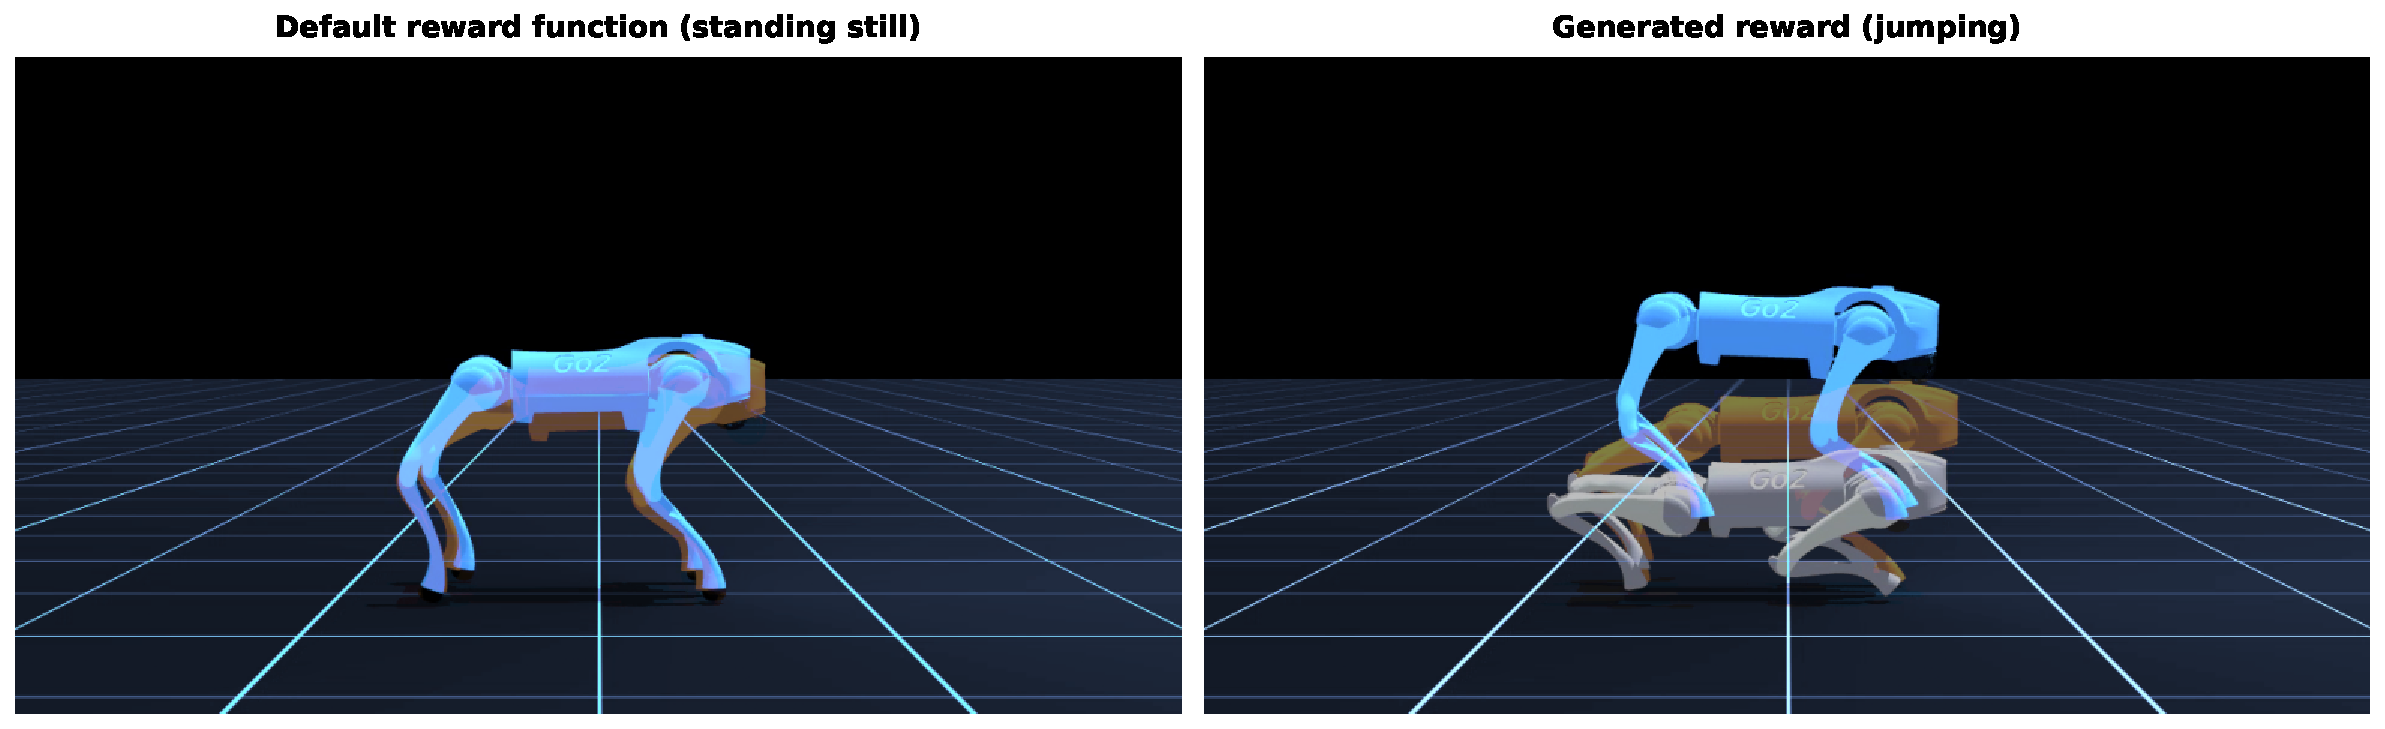
\includegraphics[width=\textwidth]{figures/genesis_robots.pdf}
\caption{Comparison between (Left) the default reward function, which leads to a stationary posture of standing tall, and (Right) a generated reward function that induces jumping behavior. The orange robot indicates the start position, the white robot indicates an intermediate position during the episode, and the blue robot indicates the end position.}
\label{fig:genesis-robots}
\end{figure}

\subsection{Olympiad-level Math Grading}
\label{app:domain-imograding}

In the Olympiad-level math grading domain, tasks are drawn from IMO-GradingBench \citep{luong2025towards}. Each task consists of an Olympiad-level math problem, a candidate solution, reference solutions, and grading guidelines. The agent is required to assign a discrete score from the set \{0, 1, 6, 7\}, corresponding to the categories \{incorrect, partial, almost, correct\}. The agent's output is a single numeric grade. Performance is measured by accuracy with respect to expert human annotations, with additional analyses provided in \Cref{app:res-imograders}. We use randomly sampled subsets of tasks for training, validation, and testing, with 100 tasks in each split. During training, an agent is first evaluated on a subset of 10 tasks (out of 100). If the agent succeeds on at least one of these tasks, it is then evaluated on the full training set.

Representative static baseline (ProofAutoGrader) from \citet{luong2025towards}:
\input{domain_imograding/proofautograder}

\section{Experiment Details}
\label{app:exp-details}

This appendix provides additional experimental details to support reproducibility and interpretation of the results. We first summarize the FMs and hyperparameters used for self-modification and task evaluation across domains (\Cref{app:fm-hyperparam}), followed by an estimate of the computational cost of running the OHM in each setting (\Cref{app:cost-estimate}). We then formally define the generate@k metric used to quantify an agent's ability to produce improved variants under a fixed budget (\Cref{app:genk-metric}). Finally, we describe the procedure used to select transfer agents for cross-domain experiments (\Cref{app:transfer-selection}).

\subsection{Hyperparameters for FMs}
\label{app:fm-hyperparam}

\Cref{tab:fm-hyperparam} summarizes the foundation models (FMs) used across experimental settings. For the Polyglot coding domain, we adopt the same FMs and temperature configurations as \citet{zhang2025darwin} to ensure a fair comparison. In all other domains, we use Claude-4.5-Sonnet for self-modification, given its strong performance on code generation tasks. For task evaluation, we select the FM based on practical considerations, including cost, rate limits, response latency, and overall task competence. In the robotics reward design setting, where the agent must implement reward functions in code, we again use Claude-4.5-Sonnet. For Olympiad-level mathematics grading, which requires substantial mathematical reasoning, we use o4-mini. The temperature is set to 0.0 for all FMs in every setting, except for o4-mini, which is fixed at 1.0.

\begin{table}[H]
\centering
\caption{Foundation models used in each experiment setting for self-modification or task evaluation.}
\label{tab:fm-hyperparam}
\begin{tabular}{@{}lll@{}}
\toprule
\multicolumn{1}{c}{\textbf{Domain}} & \multicolumn{1}{c}{\textbf{Self-modification}} & \multicolumn{1}{c}{\textbf{Evaluation}} \\ \midrule
Polyglot & Claude 3.5 Sonnet (New) & o3-mini \\
Paper review & Claude 4.5 Sonnet & GPT-4o \\
Robotics reward design & Claude 4.5 Sonnet & Claude 4.5 Sonnet \\
IMO-level grading & Claude 4.5 Sonnet & o4-mini \\ \bottomrule
\end{tabular}
\end{table}

\subsection{Cost Estimate}
\label{app:cost-estimate}

Running the OHM for 100 iterations incurs a cost of approximately USD 500 for the self-modification phase alone (excluding task evaluation). The total cost of an experiment therefore consists of the self-modification cost plus the cost of task evaluation. For the paper review and robotics reward design experiments, the evaluation cost per iteration is USD 5.10 (USD 5 for paper review evaluation + USD 0.10 for robotics reward design evaluation). Consequently, for a 100-iteration run (\Cref{sec:results}), the estimated total cost is USD 500 for self-modification plus USD 5.10 × 100 for evaluation, yielding a total of approximately USD 1,010.

A more granular break down of the task evaluation cost is:

\begin{table}[H]
\centering
\begin{tabular}{@{}cccc@{}}
\toprule
\textbf{FM} & \textbf{Benchmark} & \textbf{Number of Tasks} & \textbf{Cost Estimate (USD)} \\ \midrule
o3-mini & Polyglot & 60 & \$4 \\
GPT-4o & Paper review & 100 & \$5 \\
Claude-4.5-sonnet & Robotics reward design & 6 & \$0.10 \\
o4-mini & IMO-GradingBench & 100 & \$0.50 \\ \bottomrule
\end{tabular}
\end{table}

\subsection{Generate@k Metric}
\label{app:genk-metric}

Let $a^{0}$ denote an initial agent, $\mathcal{T}$ a fixed set of tasks, and $\mathcal{M}$ a fixed agent-generation algorithm (e.g., DGM or OHM variants). The algorithm $\mathcal{M}$ is allowed to generate up to $k$ candidate agents by iteratively applying self-modification starting from $a^{0}$.

Let
\[
\mathcal{A}^{(k)} = \{a^{1}, a^{2}, \dots, a^{k}\}
\]
denote the set of agents generated by $\mathcal{M}$ within $k$ self-modification steps. Each agent
$a \in \{a^{0}\} \cup \mathcal{A}^{(k)}$ is evaluated on the task $\mathcal{T}$ using a fixed evaluation
procedure $\mathrm{Evaluate}(\cdot, \mathcal{T})$, where higher values indicate better performance.

We define the \textbf{generate@k} metric as
\[
\mathrm{gen@}k(a^{0}, \mathcal{M}, \mathcal{T})
\;=\;
\max_{a \in \mathcal{A}^{(k)}} \mathrm{Evaluate}(a, \mathcal{T})
\;-\;
\mathrm{Evaluate}(a^{0}, \mathcal{T}).
\]

Intuitively, gen@k measures the maximum performance improvement achievable by applying the agent-generation algorithm $\mathcal{M}$ for $k$ steps starting from the initial agent $a^{0}$. Larger values of gen@k indicate stronger agent-generation capability under a fixed computational budget.

A limitation of gen@k is that it treats performance improvements as linear, without accounting for differences in difficulty across performance levels. In particular, improvements near saturation (e.g., increasing accuracy from 0.7 to 0.8) may be substantially harder to achieve than equivalent absolute gains at lower performance levels (e.g., from 0.0 to 0.1). As a result, gen@k may underestimate the significance of improvements achieved at higher performance regimes. However, this limitation does not affect the analyses presented in this work, as gen@k is used primarily for relative comparisons under matched initial conditions and fixed evaluation budgets, where all methods are subject to the same saturation effects (\Cref{sec:results-meta}).

\subsection{Transfer Agent Selection}
\label{app:transfer-selection}

To select agents for the transfer experiments (\Cref{sec:results-meta,sec:results-compound}), we use a descendant growth criterion that favors agents which serve as strong stepping stones for subsequent improvements, rather than agents that are merely high-scoring themselves.
Concretely, given the final archive at iteration \(t\),
\[
\mathcal{A}^t = \{a_1^t, a_2^t, \dots, a_N^t\},
\]
let \(\alpha_i\) denote the (aggregated) evaluation score of agent \(a_i^t\) on the source-domain validation set when available, and otherwise on the training set.
Let \(\mathrm{parent}(j)\) denote the parent of node \(j\) in the archive tree, and let \(\mathrm{dist}(i,j)\) be the number of edges on the unique path from \(i\) to descendant \(j\).

We define the \emph{growth score} of a candidate transfer node \(i\) as the discounted average improvement achieved by its descendants relative to \(i\):
\[
G_\gamma(i)
\;=\;
\frac{1}{|\mathcal{D}(i)|}
\sum_{j \in \mathcal{D}(i)}
\bigl(\alpha_j - \alpha_i\bigr)\,\gamma^{\mathrm{dist}(i,j)},
\]
where \(\mathcal{D}(i)\) is the set of descendants of \(i\) in the archive tree and \(\gamma \in (0,1]\) controls how strongly we discount improvements that occur many generations after \(i\).
Intuitively, \(G_\gamma(i)\) assigns higher weight to agents that reliably generate better descendants within fewer self-modification steps, which we treat as evidence of stronger agent-generation ability.

In our experiments, we set \(\gamma = 0.6\) and select the transfer agent by ranking nodes in descending order of \(G_{0.6}(i)\) and choosing the highest-ranked node. To reduce noise, we only compute \(G_\gamma(i)\) for nodes with at least \(m\) scored descendants (we use \(m=3\) in our implementation).

\section{Additional Results}
\label{app:res}

This appendix presents additional qualitative and diagnostic results that complement the main findings. We first highlight examples of the best task agents discovered by the OHM and describe how their behavior emerges from cumulative code changes (\Cref{app:best-agents}). We then provide qualitative analyses of how the OHM improves task performance over time across domains (\Cref{app:qual-task}) and how it develops meta-level capabilities that improve its ability to self-improve (\Cref{app:qual-meta}). We further analyze the behavior of automatically discovered Olympiad-level math graders (\Cref{app:res-imograders}) and report preliminary experiments in which the OHM is allowed to modify its own parent selection mechanism, shedding light on the limits and potential of fully self-referential optimization (\Cref{app:res-parentselect}). All experiment logs are open-sourced in our codebase.

\subsection{Best Discovered Task Agents}
\label{app:best-agents}

We show the portions of the diff patches that contribute to the task agent and are relevant to the domain. The full diff patches are open-sourced in our codebase.

\subsubsection{Paper Review}
\label{app:best-agents-paperreview}
Diff patches contributing to the best task agent discovered by the OHM (\Cref{sec:results-task}) for paper review:
\begin{lstlisting}[language=Diff]
diff --git a/task_agent.py b/task_agent.py
index 3798256..42ab625 100644
--- a/task_agent.py
+++ b/task_agent.py
@@ -5,7 +5,7 @@ from utils.common import extract_jsons
 class TaskAgent(AgentSystem):
     def forward(self, inputs):
         """
-        An agent that solves a given task.
+        An agent that solves a given task with enhanced reasoning and error handling.

         Args:
             inputs (dict): A dictionary with input data for the task.
@@ -15,30 +15,80 @@ class TaskAgent(AgentSystem):
                 - prediction (str): The prediction made by the agent.
                 - new_msg_history (list): A list of messages...
         """
-        domain = inputs['domain']
-        instruction = f"""You are an agent.
+        domain = inputs.get('domain', 'unknown')
+
+        # Enhanced instruction with chain-of-thought reasoning
+        instruction = f"""You are an expert agent solving tasks in the '{domain}' domain.

 Task input:
 ```
 {inputs}
 ```

+Please analyze this task carefully and provide your response. Follow these steps:
+1. Understand the task requirements
+2. Consider relevant approaches or solutions
+3. Provide your final answer
+
 Respond in JSON format with the following schema:
 <json>
 {{
-    "response": ...
+    "reasoning": "Brief explanation of your approach",
+    "response": "Your final answer"
 }}
-</json>"""
-        new_msg_history = chat_with_agent(instruction, ...)
+</json>
+
+Note: The 'response' field is required and should contain your answer."""
+
+        try:
+            new_msg_history = chat_with_agent(
+                instruction,
+                model=self.model,
+                msg_history=[],
+                logging=self.log
+            )
+        except Exception as e:
+            self.log(f"Error in chat_with_agent: {e}")
+            return "Error: Failed to get response from agent", []

-        # Extract the response
+        # Extract the response with improved error handling
         prediction = "None"
         try:
-            extracted_jsons = extract_jsons(new_msg_history[-1]['text'])
-            if extracted_jsons is not None and "response" in extracted_jsons[-1]:
-                prediction = extracted_jsons[-1]['response']
+            if new_msg_history and len(new_msg_history) > 0:
+                last_message = new_msg_history[-1].get('text', '')
+                extracted_jsons = extract_jsons(last_message)
+
+                if extracted_jsons is not None and len(extracted_jsons) > 0:
+                    last_json = extracted_jsons[-1]
+
+                    if "response" in last_json:
+                        prediction = last_json['response']
+                        if "reasoning" in last_json:
+                            self.log(f"Agent reasoning: {last_json['reasoning']}")
+                    else:
+                        self.log("Warning: JSON response missing 'response' field")
+                        prediction = str(last_json)
+                else:
+                    self.log("Warning: No valid JSON found in response")
+                    prediction = last_message[:500]
         except Exception as e:
             self.log(f"Error extracting prediction: {e}")
-            prediction = "None"
+            # Attempt to recover with raw response
+            try:
+                if new_msg_history and len(new_msg_history) > 0:
+                    prediction = new_msg_history[-1].get('text', 'Error')[:500]
+            except:
+                prediction = "Error: Complete extraction failure"

         return prediction, new_msg_history
\end{lstlisting}

\begin{lstlisting}[language=Diff]
diff --git a/task_agent.py b/task_agent.py
--- a/task_agent.py
+++ b/task_agent.py
@@ -17,8 +17,35 @@ class TaskAgent(AgentSystem):
         """
         domain = inputs.get('domain', 'unknown')

-        # Enhanced instruction with chain-of-thought reasoning
-        instruction = f"""You are an expert agent solving tasks...
+        # Domain-specific instructions
+        if domain == 'paper_review':
+            paper_text = inputs.get('paper_text', '')
+            instruction = f"""You are an expert reviewer evaluating academic papers.
+Your task is to decide whether to ACCEPT or REJECT the paper.
+
+Paper to review:
+```
+{paper_text}
+```
+
+Evaluate the paper based on:
+1. Novelty and originality of the research
+2. Technical soundness and methodology
+3. Experimental validation and results
+4. Clarity of presentation
+5. Significance of contributions
+
+Provide your decision in JSON format:
+<json>
+{{
+    "reasoning": "Brief explanation of your decision (2-3 sentences)",
+    "response": "accept or reject"
+}}
+</json>
+
+IMPORTANT: The 'response' field must be EXACTLY either 'accept' or 'reject'
+(lowercase, one word only)."""
+        else:
+            # Generic instruction for other domains
+            instruction = f"""You are an expert agent solving tasks in the '{domain}' domain.
\end{lstlisting}

\begin{lstlisting}[language=Diff]
diff --git a/task_agent.py b/task_agent.py
--- a/task_agent.py
+++ b/task_agent.py
@@ -20,24 +20,43 @@ class TaskAgent(AgentSystem):
         # Domain-specific instructions
         if domain == 'paper_review':
             paper_text = inputs.get('paper_text', '')
-            instruction = f"""You are an expert reviewer evaluating academic papers...
+            instruction = f"""You are a rigorous and critical academic reviewer
+evaluating papers for a top-tier conference. Your task is to decide whether to
+ACCEPT or REJECT the paper. Be skeptical and thorough.

 Paper to review:
 ```
 {paper_text}
 ```

-Evaluate the paper based on:
-1. Novelty and originality of the research
-...
+Evaluate the paper critically based on:
+1. **Novelty and Originality**: Is the contribution truly novel or incremental?
+2. **Technical Soundness**: Are methods rigorous? Any flaws in theory?
+3. **Experimental Validation**: Comprehensive? Sufficient baselines?
+4. **Clarity and Presentation**: Is writing clear? Key details missing?
+5. **Significance**: Does this advance the field meaningfully?
+
+**RED FLAGS that typically warrant REJECTION:**
+- Incremental improvements without significant novelty
+- Missing critical experimental comparisons or baselines
+- Unclear methodology or missing implementation details
+- Overclaimed contributions not supported by evidence
+- Poor writing that obscures understanding
+- Limited experimental validation or weak results
+- Lack of theoretical justification or soundness issues
+- Insufficient comparison with prior state-of-the-art
+
+**Standards for ACCEPTANCE:**
+- Clear novel contribution that advances the field
+- Rigorous methodology with sound theoretical foundation
+- Comprehensive experiments with strong results
+- Well-written with clear explanations
+- Properly compared against relevant baselines
+
+**Be Critical**: Default to REJECT unless the paper clearly meets high standards.

 Provide your decision in JSON format:
 <json>
 {{
-    "reasoning": "Brief explanation of your decision (2-3 sentences)",
+    "reasoning": "Brief critical analysis (2-3 sentences on key strengths/weaknesses)",
     "response": "accept or reject"
 }}
 </json>
\end{lstlisting}

\begin{lstlisting}[language=Diff]
diff --git a/task_agent.py b/task_agent.py
--- a/task_agent.py
+++ b/task_agent.py
@@ -20,43 +20,63 @@ class TaskAgent(AgentSystem):
         # Domain-specific instructions
         if domain == 'paper_review':
             paper_text = inputs.get('paper_text', '')
-            instruction = f"""You are a rigorous and critical academic reviewer...
+            instruction = f"""You are a critical academic reviewer for a top-tier
+conference. Use a two-stage evaluation process:

 Paper to review:
 ```
 {paper_text}
 ```

-Evaluate the paper critically based on:
-1. **Novelty and Originality**: Is the contribution truly novel?
-...
-
-**RED FLAGS that typically warrant REJECTION:**
-...
-
-**Standards for ACCEPTANCE:**
-...
-
-**Be Critical**: Default to REJECT unless the paper clearly meets high standards.
-
-Provide your decision in JSON format:
+**STAGE 1: Identify Weaknesses**
+Systematically check for these common issues:
+
+1. **Novelty Issues:**
+   - Is this just an incremental modification of existing work?
+   - Are the contributions overclaimed or trivial?
+
+2. **Methodological Flaws:**
+   - Are key implementation details missing?
+   - Are there questionable assumptions or theoretical gaps?
+
+3. **Experimental Weaknesses:**
+   - Missing important baselines or comparisons?
+   - Weak or marginal improvements?
+
+4. **Presentation Problems:**
+   - Unclear writing or poor organization?
+   - Missing critical details for reproducibility?
+
+5. **Limited Scope:**
+   - Tested only on toy problems?
+   - Narrow applicability?
+
+**STAGE 2: Make Decision**
+A paper should be **REJECTED** if:
+- It has 2 or more significant weaknesses from Stage 1
+- It has 1 critical flaw
+- The contribution is too incremental
+
+A paper should be **ACCEPTED** only if:
+- It has clear novel contributions
+- Strong experimental validation
+- Well-written and technically sound
+- At most minor, fixable issues
+
+**Critical Mindset:** Most papers have significant flaws.
+About 50% of papers should be rejected.
+
+Provide your evaluation in JSON format:
 <json>
 {{
-    "reasoning": "Brief critical analysis (2-3 sentences)",
+    "weaknesses_found": "List 2-3 main weaknesses identified in Stage 1",
+    "reasoning": "Based on the weaknesses, explain why you accept or reject",
     "response": "accept or reject"
 }}
 </json>
\end{lstlisting}

\begin{lstlisting}[language=Diff]
diff --git a/task_agent.py b/task_agent.py
--- a/task_agent.py
+++ b/task_agent.py
@@ -20,68 +20,71 @@ class TaskAgent(AgentSystem):
         # Domain-specific instructions
         if domain == 'paper_review':
             paper_text = inputs.get('paper_text', '')
-            instruction = f"""You are a critical academic reviewer...
-
-**STAGE 1: Identify Weaknesses**
-...
+            instruction = f"""You are a rigorous peer reviewer for a top-tier
+academic conference. Your reputation depends on making careful, balanced decisions.

-**STAGE 2: Make Decision**
-...
-
-Provide your evaluation in JSON format:
-<json>
-{{
-    "weaknesses_found": "List 2-3 main weaknesses identified in Stage 1",
-    "reasoning": "Based on the weaknesses, explain why you accept or reject",
-    "response": "accept or reject"
-}}
-</json>
-
-IMPORTANT: The 'response' field must be EXACTLY either 'accept' or 'reject'..."""
+**Paper to Review:**
+{paper_text}

+**Evaluation Framework:**

+**ACCEPTANCE CRITERIA (ALL must be satisfied):**
+1. **Novelty**: Presents genuinely new ideas, not incremental improvements
+2. **Technical Soundness**: Methodology is rigorous, correct, and well-justified
+3. **Significance**: Makes important contributions that advance the field
+4. **Experimental Validation**: Claims thoroughly supported with comprehensive experiments
+5. **Clarity**: Clear, well-organized presentation with proper motivation
+6. **Reproducibility**: Sufficient detail for replication
+7. **Related Work**: Proper comparison with existing methods

+**REJECTION CRITERIA (ANY one can warrant rejection):**
+- Lacks novelty; merely combines existing techniques without insight
+- Methodological flaws or incorrect technical approach
+- Insufficient experimental validation or cherry-picked results
+- Missing critical baselines or unfair comparisons
+- Overclaimed contributions not supported by evidence
+- Poor writing quality that obscures technical content
+- Ethical concerns or reproducibility issues
+- Limited scope or significance

+**Decision Guidelines:**
+- **ACCEPT**: Paper clearly satisfies ALL acceptance criteria with strong evidence
+- **REJECT**: Paper fails one or more acceptance criteria OR matches rejection criteria
+- **When in doubt, err on the side of rejection**

+**Your Review Process:**
+1. Identify the paper's main claims and contributions
+2. Evaluate each acceptance criterion systematically
+3. Check for rejection criteria
+4. Ask: "Does this paper significantly advance the field?"
+5. Make a decision based on evidence, not superficial features

+**Response Format:**
+Provide your decision in this exact JSON format:
+<json>
+{{
+    "response": "accept"
+}}
+</json>

+OR

+<json>
+{{
+    "response": "reject"
+}}
+</json>

+**CRITICAL REQUIREMENTS:**
+- The "response" field must contain ONLY "accept" or "reject" (lowercase)
+- Be thorough and critical - rejecting weak papers maintains scientific standards
+- Your decision should be defensible based on the criteria above
+- ONLY output the single word: "accept" or "reject" """
\end{lstlisting}


\subsubsection{Robotics Reward Design}
\label{app:best-agents-genesis}
Diff patches contributing to the best task agent discovered by the OHM (\Cref{sec:results-task}) for robotics reward design:
% gen_1
\begin{lstlisting}[language=Diff]
diff --git a/task_agent.py b/task_agent.py
index 3798256..98e6706 100644
--- a/task_agent.py
+++ b/task_agent.py
@@ -5,7 +5,7 @@ from utils.common import extract_jsons
 class TaskAgent(AgentSystem):
     def forward(self, inputs):
         """
-        An agent that solves a given task.
+        An agent that solves a given task with enhanced reasoning and error handling.
         ...
         """
-        domain = inputs['domain']
-        instruction = f"""You are an agent.
+        domain = inputs.get('domain', 'general')
+
+        # Enhanced instruction with clearer structure and reasoning guidance
+        instruction = f"""You are an expert AI agent specialized in solving complex tasks.

-Task input:
+Task Domain: {domain}
+
+Task Input:
 ```
 {inputs}
 ```

+Instructions:
+1. Carefully analyze the task input and identify the key requirements
+2. Break down the problem into logical steps if needed
+3. Formulate your response based on the task requirements
+4. Provide your final answer in the specified JSON format
+
 Respond in JSON format with the following schema:
 <json>
 {{
-    "response": ...
+    "reasoning": "Brief explanation of your approach",
+    "response": "Your final answer here"
 }}
-</json>"""
-        new_msg_history = chat_with_agent(instruction, model=self.model, msg_history=[], logging=self.log)
+</json>

-        # Extract the response
+IMPORTANT: Always include both 'reasoning' and 'response' fields in your JSON output."""
+
+        # Attempt to get response with retry logic
+        max_retries = 2
         prediction = "None"
-        try:
-            extracted_jsons = extract_jsons(new_msg_history[-1]['text'])
-            if extracted_jsons is not None and "response" in extracted_jsons[-1]:
-                prediction = extracted_jsons[-1]['response']
-        except Exception as e:
-            self.log(f"Error extracting prediction: {e}")
-            prediction = "None"
+        new_msg_history = []
+
+        for attempt in range(max_retries + 1):
+            try:
+                new_msg_history = chat_with_agent(...)
+                # Extract the response with retry logic
+                if new_msg_history and len(new_msg_history) > 0:
+                    extracted_jsons = extract_jsons(new_msg_history[-1]['text'])
+                    if extracted_jsons is not None and len(extracted_jsons) > 0:
+                        response_json = extracted_jsons[-1]
+                        if "reasoning" in response_json:
+                            self.log(f"Agent reasoning: {response_json['reasoning']}")
+                        if "response" in response_json:
+                            prediction = response_json['response']
+                            break
+            except Exception as e:
+                self.log(f"Error in attempt {attempt + 1}: {str(e)}")

         return prediction, new_msg_history
\end{lstlisting}

% % gen_7
% \begin{lstlisting}[language=Diff]
% diff --git a/task_agent.py b/task_agent.py
% index 98e6706..3c2dd8a 100644
% --- a/task_agent.py
% +++ b/task_agent.py
% @@ -17,8 +17,43 @@ class TaskAgent(AgentSystem):
%          """
%          domain = inputs.get('domain', 'general')

% -        # Enhanced instruction with clearer structure and reasoning guidance
% -        instruction = f"""You are an expert AI agent specialized in solving complex tasks.
% +        # Build domain-specific instruction
% +        if domain == 'paper_review':
% +            paper_text = inputs.get('paper_text', '')
% +            instruction = f"""You are an expert reviewer for a top-tier academic conference.

% +Your task is to decide whether to ACCEPT or REJECT the following paper.

% +Paper Text:
% +{paper_text}

% +Evaluation Criteria (consider ALL criteria):
% +1. **Novelty**: Does the paper present genuinely new ideas or significant contributions?
% +2. **Technical Quality**: Is the methodology sound? Are experiments well-designed?
% +3. **Clarity**: Is the paper well-written and easy to understand?
% +4. **Significance**: Will this work meaningfully impact the field?
% +5. **Validation**: Are claims properly supported by evidence?

% +Instructions:
% +1. Analyze the paper objectively against all five criteria
% +2. Identify both strengths and weaknesses
% +3. Make a balanced decision - avoid default bias toward acceptance or rejection
% +4. Base your decision on concrete evidence from the paper
% +5. Accept papers that meet high standards across most criteria
% +6. Reject papers with fatal flaws or insufficient contributions

% +Respond in JSON format:
% +<json>
% +{{
% +    "reasoning": "Balanced analysis of key strengths and weaknesses (2-4 sentences)",
% +    "response": "accept or reject (exactly one word, lowercase)"
% +}}
% +</json>

% +IMPORTANT: The response field must contain ONLY "accept" or "reject" (lowercase)."""
% +        else:
% +            # Generic instruction for other domains
% +            instruction = f"""You are an expert AI agent specialized in solving complex tasks.
% \end{lstlisting}

% gen_8
\begin{lstlisting}[language=Diff]
diff --git a/task_agent.py b/task_agent.py
index 3c2dd8a..faab41d 100644
--- a/task_agent.py
+++ b/task_agent.py
@@ -27,30 +27,96 @@ Paper Text:
+Critical Evaluation Guidelines:
+- Be rigorous and selective - most submissions have issues
+- Accept ONLY papers that are strong across MOST criteria (4-5/5)
+- Reject papers with significant weaknesses in multiple areas
+- A paper needs to be clearly above average to warrant acceptance
+- Consider: Would this paper strengthen the conference program?
+- If a paper is borderline or has major concerns, lean toward REJECT

+        elif domain == 'genesis_go2walking':
+            # Genesis domain-specific instruction with environment attribute documentation
+            task_description = inputs.get('task_description', '')
+            genesis_env_path = inputs.get('genesis_environment_path', '')
+            default_reward_function = inputs.get('default_reward_function', '')
+
+            instruction = f"""You are an expert in reinforcement learning and reward function design.

+Task: {task_description}

+Default Reward Function:
+```python
+{default_reward_function}
+```

+AVAILABLE ENVIRONMENT ATTRIBUTES (use ONLY these):
+- env.commands: [num_envs, 3] - velocity commands [lin_vel_x, lin_vel_y, ang_vel_z]
+- env.base_lin_vel: [num_envs, 3] - base linear velocity [x, y, z]
+- env.base_ang_vel: [num_envs, 3] - base angular velocity [roll, pitch, yaw]
+- env.base_pos: [num_envs, 3] - base position [x, y, z]
+- env.base_quat: [num_envs, 4] - base orientation quaternion
+- env.projected_gravity: [num_envs, 3] - gravity vector in base frame
+- env.dof_pos: [num_envs, 12] - joint positions
+- env.dof_vel: [num_envs, 12] - joint velocities
+- env.actions: [num_envs, 12] - current actions
+- env.last_actions: [num_envs, 12] - previous actions
+- env.last_dof_vel: [num_envs, 12] - previous joint velocities

+IMPORTANT CONSTRAINTS:
+- DO NOT use env.torques (not available)
+- DO NOT access undefined attributes
+- Use only the attributes listed above
+- All operations must work with PyTorch tensors
\end{lstlisting}

% gen_12
\begin{lstlisting}[language=Diff]
diff --git a/task_agent.py b/task_agent.py
index faab41d..62c444f 100644
--- a/task_agent.py
+++ b/task_agent.py
@@ -88,19 +90,24 @@ AVAILABLE ENVIRONMENT ATTRIBUTES (use ONLY these):
-IMPORTANT CONSTRAINTS:
-- DO NOT use env.torques (not available)
-- DO NOT access undefined attributes
-- Use only the attributes listed above
-- All operations must work with PyTorch tensors
+CRITICAL RULES (VIOLATION WILL CAUSE IMMEDIATE FAILURE):
+1. DO NOT reference env.torques or env.dt in your code - THESE DO NOT EXIST
+2. DO NOT add hasattr() checks for unavailable attributes and then use them
+3. DO NOT assume any attributes beyond the exact list above
+4. NEVER write code like: if hasattr(env, 'torques'): use env.torques
+5. All operations must work with PyTorch tensors
+6. If you need time differences, use fixed timestep: dt = 0.02
+7. ONLY use attributes from the AVAILABLE list - nothing else exists

+                            # Post-process prediction based on domain
+                            if domain == 'paper_review':
+                                # Ensure response is exactly "accept" or "reject"
+                                prediction_lower = str(prediction).lower().strip()
+                                if 'accept' in prediction_lower and 'reject' not in prediction_lower:
+                                    prediction = 'accept'
+                                elif 'reject' in prediction_lower:
+                                    prediction = 'reject'
+                                else:
+                                    self.log(f"Warning: Ambiguous response '{prediction}', defaulting to 'reject'")
+                                    prediction = 'reject'
\end{lstlisting}

% gen_13
\begin{lstlisting}[language=Diff]
diff --git a/task_agent.py b/task_agent.py
index 62c444f..fb504a2 100644
--- a/task_agent.py
+++ b/task_agent.py
@@ -40,26 +40,30 @@ Critical Evaluation Guidelines:
-- If a paper is borderline or has major concerns, lean toward REJECT
+- Balance your decisions: aim for appropriate selectivity (not too lenient, not too harsh)
+- If a paper is borderline, carefully weigh the evidence on both sides

 Reward Function Design Guidelines:
 1. Primary reward: Track forward velocity command (env.commands[:, 0] vs env.base_lin_vel[:, 0])
+   - Use exponential reward: torch.exp(-error * temperature) for smooth gradients
+   - Typical temperature: 1.0-2.0, scale: 0.8-1.0
 2. Secondary rewards: Track angular velocity, maintain base height, stable orientation
-3. Penalties: Excessive action changes (use env.actions - env.last_actions)
-4. Use exponential rewards: torch.exp(-error * temperature) for smooth gradients
-5. Scale rewards appropriately (main objectives: 0.5-1.0, penalties: -0.5 to -0.01)
-6. For smooth action changes: use torch.sum(torch.square(env.actions - env.last_actions))
-7. For velocity smoothness: use torch.sum(torch.square(env.dof_vel - env.last_dof_vel))
-8. Return: total_reward, reward_components dict, reward_scales dict
+   - Angular velocity tracking: similar to linear velocity
+   - Base height: penalize deviation from target (typically 0.32m)
+   - Orientation: use env.projected_gravity to penalize tilt
+3. Penalties for smooth and stable locomotion:
+   - Action smoothness: -0.01 * torch.sum(torch.square(env.actions - env.last_actions), dim=1)
+   - Joint velocity smoothness: -0.001 * torch.sum(torch.square(env.dof_vel - env.last_dof_vel), dim=1)
+   - Excessive joint velocities: -0.0005 * torch.sum(torch.square(env.dof_vel), dim=1)
+   - Unwanted lateral movement: penalize env.base_lin_vel[:, 1]
+4. Balance reward components:
+   - Main tracking objectives: 0.5-1.0 scale
+   - Secondary objectives: 0.2-0.5 scale
+   - Smoothness penalties: -0.01 to -0.001 scale
+5. Return: total_reward, reward_components dict, reward_scales dict
\end{lstlisting}

% % gen_14
% \begin{lstlisting}[language=Diff]
% diff --git a/task_agent.py b/task_agent.py
% index fb504a2..3de640e 100644
% --- a/task_agent.py
% +++ b/task_agent.py
% @@ -35,35 +35,38 @@ Evaluation Criteria (consider ALL criteria carefully):

%  Critical Evaluation Guidelines:
% -- Be rigorous and selective - most submissions have issues
% -- Accept ONLY papers that are strong across MOST criteria (4-5/5)
% -- Reject papers with significant weaknesses in multiple areas
% +- Be rigorous and selective - top conferences accept ~25% of submissions
% +- Most papers have significant issues that warrant rejection
% +- Accept ONLY papers that excel in novelty AND technical quality AND significance
% +- Even well-written papers should be rejected if they lack novelty or significance
% +- Papers must have STRONG validation with comprehensive experiments
% +- If a paper has ANY critical flaws in methodology or lacks clear novelty, REJECT
% +- For borderline cases: When in doubt between accept/reject, favor REJECT
% +- Ask yourself: Is this among the top 25% of papers? If not clearly yes, then REJECT

%  Instructions:
% -1. Critically analyze the paper against all five criteria
% -2. Identify both strengths and weaknesses objectively
% -3. Be honest about limitations - most papers have them
% +1. Start by identifying potential RED FLAGS: lack of novelty, weak validation, methodological flaws
% +2. Critically analyze against ALL five criteria - weakness in ANY major criterion -> likely REJECT
% +3. For each criterion, explicitly note whether it meets the HIGH bar for a top conference
% +4. List specific weaknesses clearly - be thorough in finding problems
% +5. Only if the paper is STRONG on novelty AND technical quality AND significance should you consider accept
% +6. Apply the "top 25% test": Would this paper be in the top quartile of all submissions?
% +7. Default stance should be critical - acceptance requires exceptional quality

%  IMPORTANT:
%  - The response field must contain ONLY "accept" or "reject" (lowercase, no other text)
% -- Provide detailed reasoning that justifies your decision
% -- Consider all five evaluation criteria in your analysis"""
% +- Start reasoning by identifying weaknesses - be thorough and critical
% +- Accept ONLY if paper excels across ALL major criteria (novelty, technical quality, significance)
% +- When uncertain or borderline, default to REJECT
% +- Remember: Most papers should be rejected; acceptance is for exceptional work only"""
% \end{lstlisting}

% % gen_16
% \begin{lstlisting}[language=Diff]
% diff --git a/task_agent.py b/task_agent.py
% index 3de640e..b39af37 100644
% --- a/task_agent.py
% +++ b/task_agent.py
% @@ -20,53 +20,49 @@ class TaskAgent(AgentSystem):
%          if domain == 'paper_review':
%              paper_text = inputs.get('paper_text', '')
% -            instruction = f"""You are an expert reviewer for a top-tier academic conference.
% +            instruction = f"""You are a reviewer for a top-tier academic conference with a ~50% acceptance rate.

% +**Evaluation Process:**

% +Score each criterion on a 3-point scale:
% +- **3 = Strong**: Exceeds expectations significantly
% +- **2 = Adequate**: Meets minimum standards but nothing exceptional
% +- **1 = Weak**: Below acceptable standards

% +**Five Criteria:**
% +1. **Novelty**: Does it present genuinely new ideas?
% +2. **Technical Quality**: Is methodology sound and rigorous?
% +3. **Clarity**: Is it well-written and clear?
% +4. **Significance**: Will it meaningfully impact the field?
% +5. **Validation**: Are claims properly validated with evidence?

% +**Decision Rules (FOLLOW STRICTLY):**
% +- **ACCEPT**: Average score >= 2.4 AND no scores of 1 on Novelty, Technical Quality, or Significance
% +- **REJECT**: Average score < 2.4 OR any score of 1 on Novelty, Technical Quality, or Significance

% +**Examples:**
% +- Scores [3,3,2,3,2] -> Average 2.6 -> ACCEPT
% +- Scores [3,2,3,2,2] -> Average 2.4 -> ACCEPT
% +- Scores [2,2,3,2,2] -> Average 2.2 -> REJECT
% +- Scores [3,1,3,3,3] -> Has 1 on Technical Quality -> REJECT
% +- Scores [2,3,2,2,2] -> Average 2.2 -> REJECT
% \end{lstlisting}

% % gen_18
% \begin{lstlisting}[language=Diff]
% diff --git a/task_agent.py b/task_agent.py
% index b39af37..7a30be1 100644
% --- a/task_agent.py
% +++ b/task_agent.py
% @@ -20,49 +20,67 @@ class TaskAgent(AgentSystem):
%          if domain == 'paper_review':
%              paper_text = inputs.get('paper_text', '')
% -            instruction = f"""You are a reviewer for a top-tier academic conference with a ~50% acceptance rate.
% +            instruction = f"""You are a CRITICAL reviewer for a top-tier conference (50% acceptance rate). Be skeptical and demand excellence.

% +**CRITICAL SCORING RUBRIC** (Be strict - most papers are NOT excellent):

% +**Score 3 (Strong)** - RARE, only for exceptional work:
% +- Novelty: Introduces fundamentally new approach/paradigm that will change how people think
% +- Technical: Methodology is impeccable with deep theoretical insights or rigorous proofs
% +- Clarity: Exceptionally clear writing that could be a textbook example
% +- Significance: Will spawn new research direction or solve major open problem
% +- Validation: Comprehensive experiments covering all edge cases with statistical rigor

% +**Score 2 (Adequate)** - Barely acceptable for publication:
% +- Novelty: Minor incremental improvement or simple combination of existing ideas
% +- Technical: Methodology is correct but straightforward, no major technical contributions
% +- Clarity: Readable but could be clearer, some concepts need better explanation
% +- Significance: Addresses niche problem with limited broader impact
% +- Validation: Basic experiments shown, but missing important ablations or baselines

% +**Score 1 (Weak)** - Below publication threshold:
% +- Novelty: No new ideas, just applies existing methods to new dataset
% +- Technical: Flawed methodology, missing baselines, or questionable assumptions
% +- Clarity: Hard to understand, poorly organized, or missing critical details
% +- Significance: Problem is trivial or solution won't impact the field
% +- Validation: Insufficient experiments, cherry-picked results, or weak evaluation

% +**RED FLAGS (Consider score 1 if ANY present):**
% +- Claims not supported by experiments
% +- Missing comparisons to obvious baselines
% +- Unclear methodology that cannot be reproduced
% +- Overclaimed significance without evidence
% +- Fundamental flaws in approach
% +- Incremental work (just benchmarking existing methods)

% +**DECISION RULES (FOLLOW EXACTLY):**
% +- **ACCEPT**: Average >= 2.5 AND all critical criteria (Novelty, Technical, Significance) >= 2
% +- **REJECT**: Average < 2.5 OR ANY of (Novelty, Technical, Significance) = 1

% +**REMEMBER:**
% +- Be CRITICAL - most papers should get 2s, not 3s
% +- Score 2 means "barely adequate", not "good"
% +- When in doubt between scores, choose the lower one
% +- ~50% of papers should be rejected"""
% \end{lstlisting}

% % gen_37
% \begin{lstlisting}[language=Diff]
% diff --git a/task_agent.py b/task_agent.py
% index 7a30be1..42c0f36 100644
% --- a/task_agent.py
% +++ b/task_agent.py
% @@ -25,48 +25,50 @@ Paper Text:

% -**CRITICAL SCORING RUBRIC** (Be strict - most papers are NOT excellent):
% +**BALANCED SCORING RUBRIC** (Be fair and objective):

% -**Score 3 (Strong)** - RARE, only for exceptional work:
% +**Score 3 (Strong)** - Clearly exceeds standards:
% +- Novelty: Presents genuinely new ideas, significant advancement over prior work
% +- Technical: Sound methodology with rigorous validation, thorough analysis
% +- Clarity: Well-written, clear presentation, reproducible methodology
% +- Significance: Addresses important problem, results will impact the field
% +- Validation: Comprehensive experiments with proper baselines and analysis

% -**Score 2 (Adequate)** - Barely acceptable for publication:
% +**Score 2 (Adequate)** - Meets publication standards:
% +- Novelty: Incremental but meaningful contribution, builds reasonably on prior work
% +- Technical: Methodology is sound though not groundbreaking, adequate rigor
% +- Clarity: Generally clear though some parts could be better explained
% +- Significance: Addresses relevant problem with reasonable impact
% +- Validation: Sufficient experiments to support claims, covers main scenarios

% -**Score 1 (Weak)** - Below publication threshold:
% +**Score 1 (Weak)** - Below publication standards:

% +**CRITICAL REJECTION CRITERIA:**
% +Reject if ANY of these are present:
% +- Fatal technical flaws or incorrect methodology
% +- Claims clearly not supported by evidence
% +- Cannot be reproduced due to missing details
% +- Novelty score = 1 (no new contribution)
% +- Technical score = 1 (fundamentally flawed)
% +- Significance score = 1 (trivial problem/solution)

% -**DECISION RULES (FOLLOW EXACTLY):**
% -- **ACCEPT**: Average >= 2.5 AND all critical criteria >= 2
% -- **REJECT**: Average < 2.5 OR ANY critical = 1
% +**DECISION RULES (FOLLOW STRICTLY):**
% +- **ACCEPT**: Average >= 2.4 AND no score of 1 on Novelty, Technical, or Significance
% +- **REJECT**: Average < 2.4 OR ANY score of 1 on Novelty, Technical, or Significance

% +**IMPORTANT REMINDERS:**
% +- Be objective and fair - evaluate each criterion independently
% +- Score 2 means "adequate/acceptable", score 3 means "strong/excellent"
% +- Focus on identifying fatal flaws (score 1) that warrant rejection
% +- Consider both strengths and weaknesses before deciding
% +- Aim for ~50% acceptance rate by being discerning but not overly harsh"""
% \end{lstlisting}

% % gen_43
% \begin{lstlisting}[language=Diff]
% diff --git a/task_agent.py b/task_agent.py
% index 42c0f36..c1c37a5 100644
% --- a/task_agent.py
% +++ b/task_agent.py
% @@ -20,70 +20,88 @@ class TaskAgent(AgentSystem):
%          if domain == 'paper_review':
%              paper_text = inputs.get('paper_text', '')
% -            instruction = f"""You are a CRITICAL reviewer for a top-tier conference (50% acceptance rate).
% +            instruction = f"""You are a RIGOROUS reviewer for a top-tier ML conference with a 25-30% acceptance rate. Most submissions have merit but only the best should be accepted.

% +**REJECTION CRITERIA** (Reject if ANY apply):
% +1. Average score < 2.5 (below quality threshold)
% +2. ANY dimension scores 1 (critical weakness)
% +3. Novelty <= 1.5 (insufficient contribution)
% +4. Technical quality = 1 (fundamentally flawed)
% +5. Claims not supported by evidence
% +6. Cannot be reproduced or validated

% +**ACCEPTANCE CRITERIA** (ALL must be satisfied):
% +1. Average score >= 2.5
% +2. NO score of 1 in any dimension
% +3. Novelty >= 2 (meaningful contribution)
% +4. Technical >= 2 (sound methodology)
% +5. Claims properly supported

% +**REVIEW PROCESS:**
% +1. Carefully read the paper and identify its main contribution
% +2. Score EACH dimension independently (don't let one dimension bias others)
% +3. Be CRITICAL: Look for weaknesses, gaps, missing comparisons
% +4. Check if rejection criteria are met (if yes, must reject)
% +5. Check if ALL acceptance criteria are met (if not all, must reject)
% +6. Calculate average and make final decision

% +**IMPORTANT:**
% +- Default to REJECT unless paper clearly meets ALL acceptance criteria
% +- ~70% of papers should be rejected (maintain high standards)
% +- Score 2 = "acceptable but not great", Score 3 = "genuinely strong"
% +- Most papers will have mix of 2s and 3s, with occasional 1s
% +- Don't be overly generous - top conferences reject many good papers
% \end{lstlisting}

% % gen_89
% \begin{lstlisting}[language=Diff]
% diff --git a/task_agent.py b/task_agent.py
% index c1c37a5..bacc897 100644
% --- a/task_agent.py
% +++ b/task_agent.py
% @@ -20,88 +20,73 @@ class TaskAgent(AgentSystem):
%          if domain == 'paper_review':
%              paper_text = inputs.get('paper_text', '')
% -            instruction = f"""You are a RIGOROUS reviewer for a top-tier ML conference with a 25-30% acceptance rate.
% +            instruction = f"""You are a reviewer for a top-tier ML/AI conference with approximately 50% acceptance rate.

% +**Review Philosophy:**
% +- Be fair and balanced: recognize both strengths and weaknesses
% +- Most papers submitted to top venues have merit - distinguish publishable from not-yet-ready
% +- Use the full 1-3 scale: avoid clustering scores (distribute naturally)
% +- Score 2 is the "default acceptable" level - most criteria will be 2 or 3
% +- Reserve score of 1 for truly serious flaws only

% +**Scoring Scale (Be Generous but Fair):**
% +- **3 = Good/Strong**: Clear strengths on this criterion, above average quality
% +- **2 = Acceptable/Adequate**: Meets publication standards, no major issues
% +- **1 = Poor/Inadequate**: Serious problems that disqualify the paper

% +**Five Evaluation Criteria (score each 1-3):**
% +1. **Novelty**: Is the contribution sufficiently novel? (2=incremental but solid, 3=novel idea)
% +2. **Technical Quality**: Is methodology sound? (2=adequate rigor, 3=excellent execution)
% +3. **Clarity**: Is it well-written? (2=understandable with minor issues, 3=very clear)
% +4. **Significance**: Does it matter? (2=useful contribution, 3=important impact)
% +5. **Validation**: Are claims supported? (2=adequate evidence, 3=thorough validation)

% +**Decision Rules (Apply EXACTLY):**
% +1. Calculate average of all 5 scores
% +2. Check for any fatal flaws (score of 1 on Novelty, Technical Quality, OR Significance)
% +3. **ACCEPT** if: Average >= 2.2 AND no fatal flaws (score of 1 on critical criteria)
% +4. **REJECT** if: Average < 2.2 OR has fatal flaw on critical criterion

% +**Scoring Calibration (Target 50% acceptance):**
% +ACCEPT examples:
% +- [3,3,3,2,2] -> Avg=2.6 -> ACCEPT (strong paper)
% +- [3,2,2,3,2] -> Avg=2.4 -> ACCEPT (good overall)
% +- [2,3,2,2,2] -> Avg=2.2 -> ACCEPT (meets threshold)
% +- [2,2,3,2,2] -> Avg=2.2 -> ACCEPT (adequate)
% +- [2,2,2,3,2] -> Avg=2.2 -> ACCEPT (borderline but acceptable)

% +REJECT examples:
% +- [2,2,2,2,1] -> Avg=1.8 -> REJECT (below threshold)
% +- [2,2,1,2,2] -> Avg=1.8 -> REJECT (below threshold)
% +- [3,1,3,3,2] -> REJECT (fatal flaw: Technical Quality = 1)
% +- [1,3,3,2,3] -> REJECT (fatal flaw: Novelty = 1)
% +- [2,2,2,2,2] -> Avg=2.0 -> REJECT (below threshold)

% +**Critical Guidance:**
% +- **Default to score of 2** for most criteria unless there's a clear reason for 1 or 3
% +- Score 3: Clear strength or excellence on this dimension
% +- Score 2: Acceptable quality, publishable standard (MOST COMMON)
% +- Score 1: Major flaw or serious inadequacy (RARE - use sparingly)
% +- Don't look for perfection - accept solid, publishable work
% +- The 2.2 threshold with proper scoring yields ~50% acceptance
% +- Be generous with 2s and 3s; reserve 1s for truly poor work

% +IMPORTANT:
% +- Most papers should get mostly 2s and 3s (score 1 is rare)
% +- Calculate average correctly (sum/5)
% +- Apply decision rules exactly: avg >= 2.2 AND no fatal flaws -> ACCEPT
% +- Response field: ONLY "accept" or "reject" (lowercase, no other text)"""
% \end{lstlisting}


\subsubsection{Olympiad-level Math Grading}
\label{app:best-agents-imograding}
Diff patches contributing to the best task agent discovered by the OHM with transfer from ProofAutoGrader (\Cref{sec:results-compound}) for Olympiad-level math grading:
% gen_3
\begin{lstlisting}[language=Diff]
diff --git a/task_agent.py b/task_agent.py
index 9ab8761..c00d167 100644
--- a/task_agent.py
+++ b/task_agent.py
@@ -11,10 +11,25 @@ Keep in mind the standards at the IMO are extremely high...

 ### General Scoring Rubric
 Scores are assigned on a 0-7 scale. The general guidelines are:
-* **7 Points (Correct):** The solution is complete, correct, and fully rigorous...
-* **6 Points (Almost Correct):** The solution is almost correct with a sound core argument, but contains minor errors...
-* **1 Point (Partial Progress):** The solution demonstrates substantial progress explicitly mentioned in the grading guidelines...
-* **0 Points (Incorrect):** The solution doesn't make substantial progress...
+
+* **7 Points (Correct):** The solution is complete, correct, and fully rigorous with no gaps or errors. All major steps are proven with full rigor. Every claim is justified or routine to verify...
+
+* **6 Points (Almost Correct):** The solution has ALL the major ideas and the core argument structure is sound, but contains ONE OR MORE of these minor issues:
+  - Minor algebraic/arithmetic errors that don't affect the main argument
+  - Small logical gaps that are straightforward to fill
+  - Missing routine verifications that an expert could easily supply
+  - **NOT eligible for 6 points**: Missing proofs for major lemmas, unjustified non-trivial claims, incomplete case analysis, or fundamental logical gaps
+  - **Key test**: Would an expert say "this is essentially correct, just needs minor cleanup"?
+
+* **1 Point (Partial Progress):** The solution demonstrates substantial progress on a KEY component that is explicitly mentioned in the grading guidelines for partial credit.
+  - **CRITICAL**: Carefully read the Specific Grading Guidelines section to see what counts as partial credit
+  - The solution must achieve one of the specific milestones listed in the guidelines
+  - Must make non-trivial progress toward the solution (not just initial observations)
+  - Reformulating the problem without making substantive headway is NOT sufficient
+  - Proving lemmas NOT mentioned in grading guidelines is NOT sufficient
+  - **If the guidelines list specific achievements for partial credit and the solution achieves ANY of them, award 1 point**
+
+* **0 Points (Incorrect):** The solution doesn't make substantial progress on key steps mentioned in grading guidelines, is fundamentally flawed, or makes only trivial observations.

 ### Evaluation Process
 You must follow this structured process:
-1. **Analyze References:** Meticulously read and understand the problem...
-2. **Step-by-Step Verification:** Verify the logical validity and rigor of every step...
-3. **Assess Progress:** Determine the extent of non-trivial progress made.
-4. **Score Determination:** Compare the findings against the Specific Grading Guidelines...
+
+1. **Analyze References:** Meticulously read and understand the problem and Ground Truth Solution. Carefully review the Specific Grading Guidelines to identify:
+   - The key steps required for a complete solution
+   - **What specific progress qualifies for partial credit (1 point)** - this is crucial!
+   - What distinguishes "almost correct" (6 points) from "correct" (7 points)
+
+2. **Step-by-Step Verification:** Verify the logical validity and rigor of EVERY step in the proposed solution:
+   - Identify ALL flaws, gaps, assumptions, and errors
+   - Check if gaps are "minor and routine" (possibly 6 pts) or "major" (0-1 pts)
+   - **Be careful**: Some solutions may appear correct but have hidden gaps or unjustified leaps
+   - Distinguish between minor calculation errors vs fundamental logical flaws
+
+3. **Assess Progress Against Grading Guidelines:**
+   - **Does the solution achieve the specific milestones mentioned for partial credit?**
+   - Does it have all major components with only minor fixable issues (6 points)?
+   - Or does it have complete rigor with no gaps (7 points)?
+
+4. **Score Determination:** Apply this decision tree:
+   - **If solution is complete and rigorous with no errors or gaps -> 7 points**
+   - **If solution has all major ideas but minor fixable issues -> 6 points**
+   - **If solution makes substantial progress mentioned in grading guidelines -> 1 point**
+   - **Otherwise -> 0 points**

+### Critical Reminders for Accurate Grading
+
+**Common Grading Errors to AVOID:**
+1. **Being too lenient with 7 points**: If there are ANY gaps (even minor ones that need filling), it's 6 points, not 7.
+2. **Missing partial credit**: Check the grading guidelines carefully - if the solution achieves ANY milestone mentioned for partial credit, award 1 point.
+3. **Confusing "good attempt" with "almost correct"**: 6 points requires ALL major ideas to be present, not just a good start.
+4. **Ignoring unjustified claims**: Statements like "it's easy to see" or "clearly" must actually be clear/easy. If non-trivial, it's a gap.

+**Score Distribution Calibration:**
+- Most solutions will be 0 or 7 points (either fundamentally flawed or correct)
+- 6 points should be rare (only when truly "almost there" with all ideas present)
+- 1 point should match specific milestones in grading guidelines
+- When in doubt, be strict: IMO standards are extremely high
\end{lstlisting}

% gen_9
\begin{lstlisting}[language=Diff]
diff --git a/task_agent.py b/task_agent.py
index c00d167..72475b6 100644
--- a/task_agent.py
+++ b/task_agent.py
@@ -28,8 +28,11 @@ Scores are assigned on a 0-7 scale...
   - Proving lemmas NOT mentioned in grading guidelines is NOT sufficient
   - **If the guidelines list specific achievements for partial credit and the solution achieves ANY of them, award 1 point**
+  - **IMPORTANT**: Even if the solution has major flaws or is incomplete, if it achieves ANY specific milestone from the guidelines, it deserves 1 point, not 0

 * **0 Points (Incorrect):** The solution doesn't make substantial progress...
+  - **CRITICAL CHECK**: Before assigning 0 points, verify that the solution does NOT achieve ANY of the partial credit milestones listed in the grading guidelines
+  - If even ONE milestone is achieved, the score should be 1 point, not 0

+3. **MANDATORY Partial Credit Milestone Check:**
+   - **THIS STEP IS REQUIRED - DO NOT SKIP**
+   - List each partial credit milestone explicitly from the grading guidelines
+   - For EACH milestone, determine: Does the solution achieve this? YES/NO
+   - If ANY milestone shows YES -> the score must be at least 1 point
+   - This check must happen BEFORE considering 0 points

+5. **Score Determination:** Apply this decision tree:
+   - **FIRST**: Did the solution achieve ANY partial credit milestone from the guidelines?
+     - If YES -> Score is AT LEAST 1 point (proceed to check for higher scores)
+     - If NO -> Score is 0 points (stop here)
+
+   - **If score >= 1, check for higher scores:**
+     - Is the solution complete and rigorous with no errors or gaps? -> 7 points
+     - Does it have ALL major ideas with only minor fixable issues? -> 6 points
+     - Otherwise -> 1 point

+**REQUIRED EVALUATION FORMAT:**
+You MUST structure your response as follows:
+
+1. **List Partial Credit Milestones**: Explicitly list each milestone from the grading guidelines
+2. **Check Each Milestone**: For each milestone, state whether the solution achieves it (YES/NO)
+3. **Determine Minimum Score**: If ANY milestone is YES, the minimum score is 1 point
+4. **Detailed Analysis**: Provide your complete evaluation
+5. **Final Score**: Provide the score in the required format
\end{lstlisting}

% gen_48
\begin{lstlisting}[language=Diff]
diff --git a/task_agent.py b/task_agent.py
index 72475b6..62e975b 100644
--- a/task_agent.py
+++ b/task_agent.py
+* **7 Points (Correct):** The solution is complete, correct, and fully rigorous with no gaps or errors. All major steps are proven with full rigor. Every claim is justified or truly routine to verify...
+  - **Critical requirements**: Solution must (1) address ALL parts of the problem, (2) prove ALL necessary claims, and (3) have NO unjustified leaps
+  - Every "clearly" or "obviously" must be genuinely trivial to an IMO expert
+  - All edge cases, special cases, and boundary conditions must be handled

+* **6 Points (Almost Correct):** The solution has ALL the major ideas and the core argument structure is sound, but contains ONE OR MORE of these **minor** issues:
+  - Minor algebraic/arithmetic errors that don't affect the main argument (e.g., writing 2n+1 instead of 2n+2 but the logic still holds)
+  - Small logical gaps that are straightforward to fill (e.g., "clearly" statements that are indeed clear to an expert)
+  - Missing routine verifications that an expert could easily supply (e.g., obvious algebra steps)
+  - **NOT eligible for 6 points**: Missing proofs for major lemmas, unjustified non-trivial claims, incomplete case analysis, fundamental logical gaps, or missing key components
+  - **Key test**: Would an expert say "this is essentially correct, just needs minor cleanup"? The solution structure is complete and sound.
+  - **Example of 6 points**: A proof that has all the right ideas and structure but makes a small computational error that doesn't invalidate the approach
+  - **Example of NOT 6 points**: A proof that sketches the right approach but leaves out the proof of a crucial intermediate result

+2. **Step-by-Step Verification:** Verify the logical validity and rigor of EVERY step in the proposed solution:
+   - Identify ALL flaws, gaps, assumptions, and errors
+   - For EACH "clearly" or "obviously" statement: Is it truly routine or does it hide significant work?
+   - Check if gaps are "minor and routine" (possibly 6 pts) or "major" (0-1 pts)
+   - **Be careful**: Some solutions may appear correct but have hidden gaps or unjustified leaps
+   - Distinguish between minor calculation errors vs fundamental logical flaws
+   - **Rigor check**: Are intermediate results properly proven? Are all cases covered? Are inequalities/equalities justified?

+4. **Assess Overall Quality and Completeness:**
+   - **For 7 points**: Check that EVERY claim is proven, EVERY case is handled, NO unjustified leaps exist
+   - **For 6 points**: Verify ALL major components are present and the solution structure is complete (not just a good start)
+   - **For 1 point**: Confirm at least ONE specific milestone from guidelines is achieved
+   - **For 0 points**: Verify NO milestones from guidelines are achieved

+**Examples to Calibrate Your Judgment:**
+- **7 points**: "The proof correctly establishes X by showing Y, handles all cases including Z, and proves every intermediate claim with full rigor."
+- **6 points**: "The proof has the complete structure and all major steps, but writes 'it is clear that' for a non-trivial step that needs 2-3 lines to verify."
+- **1 point**: "The solution proves Lemma A which is specifically mentioned in grading guidelines as worth partial credit, but doesn't complete the full proof."
+- **0 points**: "The solution makes interesting observations and tries several approaches, but doesn't achieve any of the specific milestones listed in the guidelines."
\end{lstlisting}

% gen_54
\begin{lstlisting}[language=Diff]
diff --git a/task_agent.py b/task_agent.py
index 62e975b..a033aa1 100644
--- a/task_agent.py
+++ b/task_agent.py
+### CRITICAL: Four-Category Classification System
+
+Before diving into details, first classify the solution into ONE of these four categories:
+
+1. **COMPLETE & RIGOROUS**: Has all components, all proofs, handles all cases, no gaps -> 7 points
+2. **NEARLY COMPLETE**: Has complete structure + all major ideas, only minor polish needed -> 6 points (RARE: ~5%)
+3. **MEANINGFUL PROGRESS**: Achieves at least ONE specific milestone from grading guidelines -> 1 point (~25%)
+4. **INSUFFICIENT**: No specific milestones achieved, only trivial observations -> 0 points
+
+**Key Decision Points:**
+- 7 vs 6: "Any gaps at all, even fixable ones?" If yes -> 6
+- 6 vs 1: "Complete proof structure with ALL major steps present?" If no -> must be 1 or 0
+- 1 vs 0: "Achieves ANY milestone listed in guidelines?" If no -> 0

+* **1 Point (Partial Progress):** The solution demonstrates substantial progress on a KEY component that is explicitly mentioned in the grading guidelines for partial credit.
+  - **CRITICAL**: You MUST check the "Specific Grading Guidelines" section below - it lists EXACTLY what qualifies for partial credit
+  - The solution must achieve at least ONE of the specific milestones listed in those guidelines
+  - **IMPORTANT DISTINCTIONS**:
+    * DOES count: Achieving a milestone listed in the guidelines (even with errors elsewhere)
+    * Does NOT count: General progress, clever observations, or lemmas NOT in the guidelines
+    * Does NOT count: Reformulating the problem without substantive progress
+    * Does NOT count: Incorrect attempts that seem "on the right track"
+  - **Examples of valid partial credit**:
+    * Guidelines say "partial credit for proving Lemma X" -> solution proves Lemma X correctly -> 1 point
+    * Guidelines say "partial credit for establishing the recurrence relation" -> solution establishes it -> 1 point
+  - **Examples that do NOT qualify for partial credit**:
+    * Solution tries several approaches but none matches a guideline milestone -> 0 points
+    * Solution proves a useful lemma not mentioned in guidelines -> 0 points (no matter how clever)
+    * Solution has the "right idea" but doesn't complete any guideline milestone -> 0 points

+**Common Grading Errors to AVOID (based on actual evaluation data):**
+
+1. **ERROR #1: Missing partial credit (11 cases last eval - partial -> incorrect)**
+   - MISTAKE: Marking solutions as 0 points that actually achieve guideline milestones
+   - FIX: Before assigning 0, explicitly list EACH milestone and check if achieved
+   - **Process**: "Does solution achieve milestone 1? NO. Milestone 2? NO. ..." Only if ALL are NO -> 0 points
+
+2. **ERROR #2: Awarding partial to incorrect solutions (7 cases - incorrect -> partial)**
+   - MISTAKE: Giving 1 point for "interesting work" or "right direction" not in guidelines
+   - FIX: Only award 1 point if solution achieves an EXACT milestone listed in guidelines
+
+3. **ERROR #3: Confusing "almost" with "correct" (5 cases - almost -> correct)**
+   - MISTAKE: Awarding 7 points when gaps exist (even minor, fillable gaps)
+   - FIX: If ANY gap needs filling (even routine) -> 6 points, NOT 7
+
+4. **ERROR #4: Over-rewarding partial progress (5 cases - partial -> correct)**
+   - MISTAKE: Awarding 7 points to solutions that achieve only some milestones
+   - FIX: Check if solution solves ENTIRE problem or just proves partial results

+5. **ERROR #5: Over-using 6 points**
+   - MISTAKE: Awarding 6 for "good progress" or "most of the way there"
+   - FIX: 6 requires COMPLETE solution structure with ALL major steps, just minor polish needed
+   - **Frequency check**: 6 points should be RARE (~5% of solutions)

+**Score Distribution Calibration (Expected Distribution):**
+- ~35% score 7 (correct): Complete, rigorous solutions with no gaps
+- ~35% score 0 (incorrect): No guideline milestones achieved
+- ~24% score 1 (partial): Achieve at least one specific guideline milestone
+- ~6% score 6 (almost): RARE - complete structure with only minor fixable issues
\end{lstlisting}

% gen_56
\begin{lstlisting}[language=Diff]
diff --git a/task_agent.py b/task_agent.py
index a033aa1..86320b1 100644
--- a/task_agent.py
+++ b/task_agent.py
 **Key Decision Points:**
 - 7 vs 6: "Any gaps at all, even fixable ones?" If yes -> 6
 - 6 vs 1: "Complete proof structure with ALL major steps present?" If no -> must be 1 or 0
-- 1 vs 0: "Achieves ANY milestone listed in guidelines?" If no -> 0
+- **1 vs 0 (MOST CRITICAL)**: "Does the solution EXPLICITLY ACHIEVE any milestone from the grading guidelines?"
+  * Read each milestone carefully and check if solution PROVES/ESTABLISHES it
+  * "Attempts" or "makes progress toward" a milestone != ACHIEVES it
+  * Must have concrete proof/result that matches milestone description
+  * If uncertain, re-read the milestone requirements and check for explicit completion

+    * Does NOT count: Stating a result without proving it
+    * Does NOT count: Getting "close" to a milestone but not completing it
+    * Solution states a milestone result but doesn't prove it -> 0 points
+    * Solution proves 80% of what's needed for a milestone -> 0 points (must be complete)
+  - **VERIFICATION CHECKLIST for each milestone**:
+    1. What exactly does the milestone require?
+    2. Does the solution provide a complete proof/derivation of this?
+    3. Are there any gaps or unjustified steps in achieving this milestone?
+    4. If there are gaps, is the milestone still considered "achieved"? (Usually NO)

+2. **Check Each Milestone**: For each milestone, systematically verify:
+   - What the milestone requires (quote from guidelines)
+   - What the solution provides (specific evidence)
+   - Does it FULLY achieve the milestone? (YES/NO with clear reasoning)
+   - Key distinction: "attempts" or "partial progress" toward milestone = NO

+**CRITICAL REMINDER FOR MILESTONE CHECKING:**
+- Be precise: A milestone is achieved only if the solution COMPLETES what the milestone describes
+- Common mistake: Giving credit for "working toward" a milestone (this should be 0 points)
+- When in doubt: Re-read the milestone requirement and check if solution fully satisfies it
\end{lstlisting}

% gen_71
\begin{lstlisting}[language=Diff]
diff --git a/task_agent.py b/task_agent.py
index 86320b1..f1dd3ac 100644
--- a/task_agent.py
+++ b/task_agent.py
 Before diving into details, first classify the solution into ONE of these four categories:

-1. **COMPLETE & RIGOROUS**: Has all components, all proofs, handles all cases, no gaps -> 7 points
+1. **COMPLETE & RIGOROUS**: Has all components, all proofs, handles all cases, ZERO gaps -> 7 points
 2. **NEARLY COMPLETE**: Has complete structure + all major ideas, only minor polish needed -> 6 points (RARE: ~5%)
 3. **MEANINGFUL PROGRESS**: Achieves at least ONE specific milestone from grading guidelines -> 1 point (~25%)
 4. **INSUFFICIENT**: No specific milestones achieved, only trivial observations -> 0 points

 **Key Decision Points:**
-- 7 vs 6: "Any gaps at all, even fixable ones?" If yes -> 6
+- **7 vs 6 (CRITICAL - BE STRICT)**: "Is this solution PUBLICATION-READY with ZERO gaps, ZERO unjustified steps, ZERO hand-waving?"
+  * ANY gap, even minor -> automatically 6 points maximum
+  * ANY "clearly", "obviously", "it follows" that needs verification -> 6 points
+  * ANY missing routine verification -> 6 points
+  * ANY computational error, however minor -> 6 points
+  * 7 points requires PERFECTION - when in doubt, give 6 points
 - 6 vs 1: "Complete proof structure with ALL major steps present?" If no -> must be 1 or 0
-- **1 vs 0 (MOST CRITICAL)**: "Does the solution EXPLICITLY ACHIEVE any milestone from the grading guidelines?"
+- **1 vs 0**: "Does the solution EXPLICITLY ACHIEVE any milestone from the grading guidelines?"
   * Read each milestone carefully and check if solution PROVES/ESTABLISHES it
   * "Attempts" or "makes progress toward" a milestone != ACHIEVES it
   * Must have concrete proof/result that matches milestone description

-* **7 Points (Correct):** The solution is complete, correct, and fully rigorous with no gaps or errors...
+* **7 Points (Correct):** The solution is complete, correct, and fully rigorous with ABSOLUTELY NO gaps or errors. All major steps are proven with full rigor. Every claim is justified or truly routine to verify...
+  - **Critical requirements**: Solution must (1) address ALL parts of the problem, (2) prove ALL necessary claims with full detail, and (3) have NO unjustified leaps whatsoever
+  - Every "clearly" or "obviously" must be genuinely trivial to an IMO expert - if it takes >30 seconds to verify, it's not trivial
+  - All edge cases, special cases, and boundary conditions must be explicitly handled
+  - **BE EXTREMELY STRICT**: 7 points should be RARE (target: ~30-40% of solutions). Most good solutions have minor gaps -> give 6 points

-* **6 Points (Almost Correct):** The solution has ALL the major ideas and the core argument structure is sound...
+* **6 Points (Almost Correct):** The solution has ALL the major ideas and the COMPLETE argument structure, but contains ONE OR MORE of these **minor** issues:
   - Minor algebraic/arithmetic errors that don't affect the main argument
-  - Small logical gaps that are straightforward to fill
+  - Small logical gaps that are straightforward to fill (e.g., "clearly" statements that need 1-2 lines to verify)
   - Missing routine verifications that an expert could easily supply
+  - Citations of standard theorems without proof (acceptable at IMO level)
   - **NOT eligible for 6 points**: Missing proofs for major lemmas, unjustified non-trivial claims, incomplete case analysis, fundamental logical gaps, or missing key components
   - **Key test**: Would an expert say "this is essentially correct, just needs minor cleanup"? The solution structure is complete and sound.
+  - **IMPORTANT**: 6 points means the solution is COMPLETE but not PERFECT. If major steps are missing -> give 1 point instead.

 * **1 Point (Partial Progress):** The solution demonstrates substantial progress on a KEY component...
   - **IMPORTANT DISTINCTIONS**:
     * DOES count: Achieving a milestone listed in the guidelines (even with errors elsewhere)
+    * DOES count: Equivalent formulations of guideline milestones (recognize reformulations)
     * Does NOT count: General progress, clever observations, or lemmas NOT in the guidelines
     * Does NOT count: Reformulating the problem without substantive progress
     * Does NOT count: Incorrect attempts that seem "on the right track"
     * Solution proves a useful lemma not mentioned in guidelines -> 0 points (no matter how clever)
+  - **When grading partial credit, be MORE LENIENT**: If the solution substantially achieves a milestone (even with minor gaps), give the point
\end{lstlisting}


\subsection{Qualitative: Improving Task Performance}
\label{app:qual-task}

Here we provide a qualitative view of how the OHM improves task performance over time by visualizing the archive trees and progress plots for one run in each setting (\Cref{sec:results}). For each domain, we annotate key nodes in the archive with the code changes that affected the behavior of the task agent only for the domain being analyzed. Across diverse domains (i.e., paper review, robotics reward design, and Olympiad-level math grading), the OHM consistently demonstrates the ability to self-improve in meaningful ways (\Cref{fig:task-paperreview,fig:task-genesis,fig:task-imograding}). Notably, many lineage paths leading to the final best-performing agent pass through intermediate nodes with lower performance, illustrating the benefits of open-ended search, which explores a diverse set of promising stepping stones rather than exclusively branching from the current best solution.

\textbf{Use structured processes, not attitude instructions.} In the paper review domain, the OHM transitions from behavioral prompting to structurally grounded decision-making \Cref{fig:task-paperreview}. In generation 39, the agent attempted to improve performance by adopting a ``rigorous and critical'' reviewer persona, encouraging stricter standards and default rejection. Subsequent analysis showed that such attitude-based instructions were unreliable, leading to a key insight in generation 54: ``for LLMs, use structured processes, not attitude instructions''. The OHM therefore introduced a two-stage evaluation procedure in which the agent first identifies weaknesses using an explicit checklist and only then makes an accept/reject decision based on predefined rules. This shift from behavioral guidance to process-level structure enabled more stable and higher-performing review behavior in later generations.

\textbf{Accumulating domain knowledge.} In robotics reward design, the most impactful changes stem from progressively grounding the agent in accurate domain knowledge (\Cref{fig:task-genesis}). A major breakthrough in generation 8 added comprehensive documentation of the target environment, explicitly listing valid state variables and constraints and providing high-level reward design guidelines, which eliminated failures caused by hallucinated attributes. Later generations (12 and 13) iteratively refined this documentation by tightening constraints, adding concrete code examples, and specifying typical reward formulations and scaling ranges. Rather than isolated prompt edits, the OHM continuously improved a shared, example-driven knowledge base that supported increasingly effective reward design.

\textbf{Automated rubrics and decision tree.} For Olympiad-level math grading, the OHM shows a steady move toward explicit evaluation structure (\Cref{fig:task-imograding}). In generation 3, listing grading categories with clear definitions corrected the tendency to solve problems instead of grading them. Subsequent generations (18 and 37) refined these categories with systematic decision procedures, calibration, and concrete boundary-case examples. Generation 168 introduced explicit rubrics, per-item checklists, and a decision-tree framework mapping rubric satisfaction to final grades, replacing descriptive guidance with precise logical flow and substantially improving grading consistency.
Rather than relying on human-designed rubrics, the OHM autonomously discovers evaluative structures that mirror those used in recent rubric-based approaches to improve consistency and interpretability in complex judgments \citep{cook2024ticking, fan2024sedareval, chen2026automated, lv2026rubrics}.

Features implemented in a given generation are often inspired by, enabled by, or recombined from mechanisms discovered in earlier generations. For example, while the agent in (\Cref{fig:task-imograding}) appears to require only five code edits to achieve the best performance in that run, these edits were in fact inspired by insights and infrastructure developed in previous generations. This kind of cumulative learning is enabled by the OHM's meta-level improvements (e.g., evaluation analysis utilities, persistent memory, performance tracking) (\Cref{app:qual-meta}). Together, these qualitative results show that the OHM's gains do not arise from isolated, single-step changes, but instead emerge from open-ended cumulative improvements in both task-level behavior and the meta-level machinery that generates those behaviors.

\begin{figure}[H]
\centering
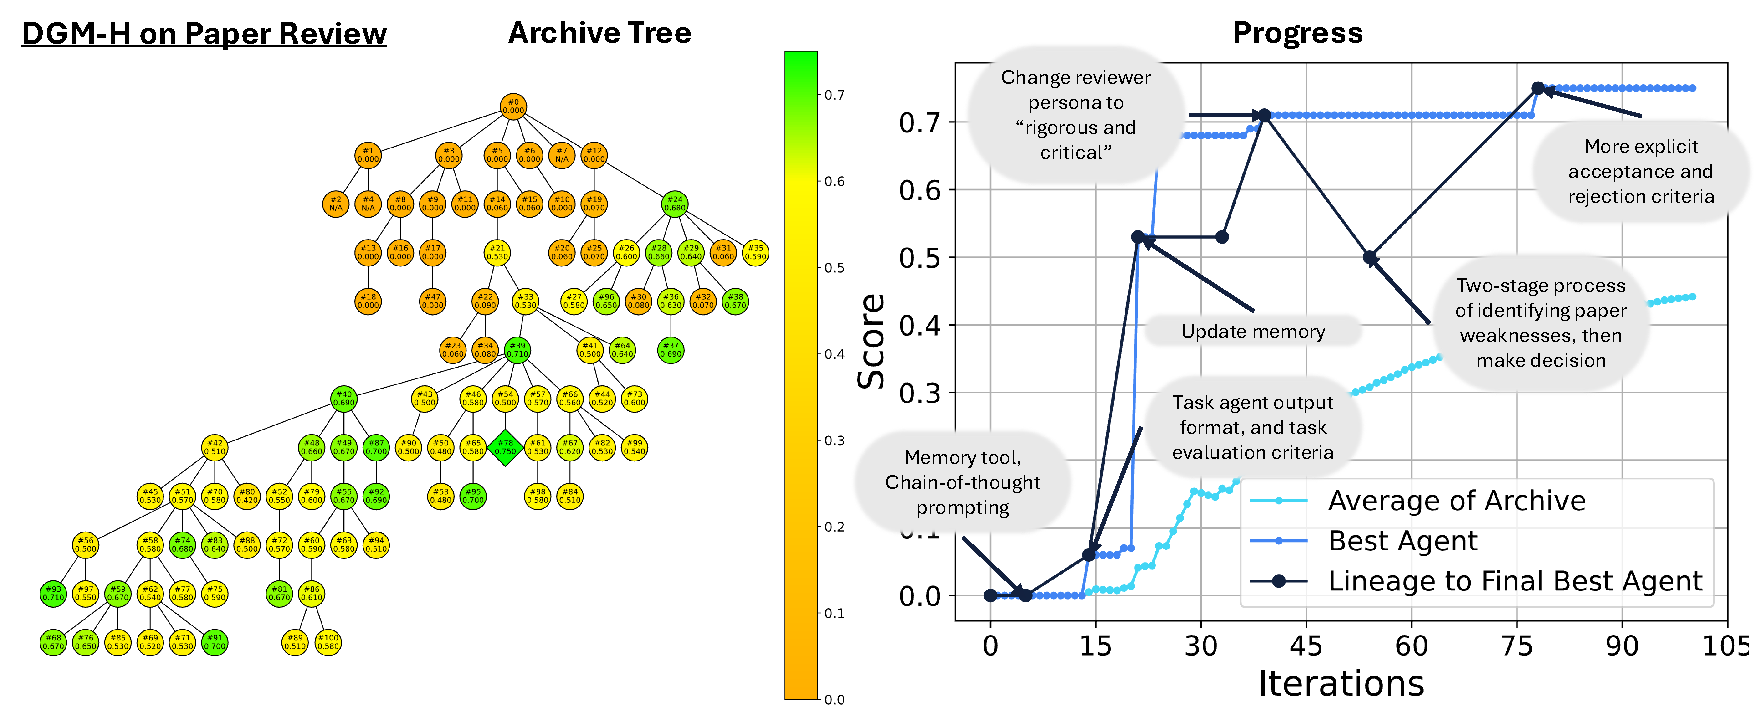
\includegraphics[width=\textwidth]{figures/results_paperreview.pdf}
\caption{\textbf{The OHM automatically self-improves to become better at paper review.} (Left) Archive of agents generated during the OHM run on paper review and robotics reward design together. Each node represents an agent, with node 0 corresponding to the initial agent. Node color indicates performance on paper review. The best-performing node is shown as a diamond. Edges show which agents self-modified to produce offspring. (Right) Progress plot of OHM on paper review. The light blue line shows the average score of all compiled agents. The blue line tracks the best score achieved by any agent in the archive at each iteration. The dark line shows the lineage of the final best-discovered agent and its precursor nodes.}
\label{fig:task-paperreview}
\end{figure}

\begin{figure}[H]
\centering
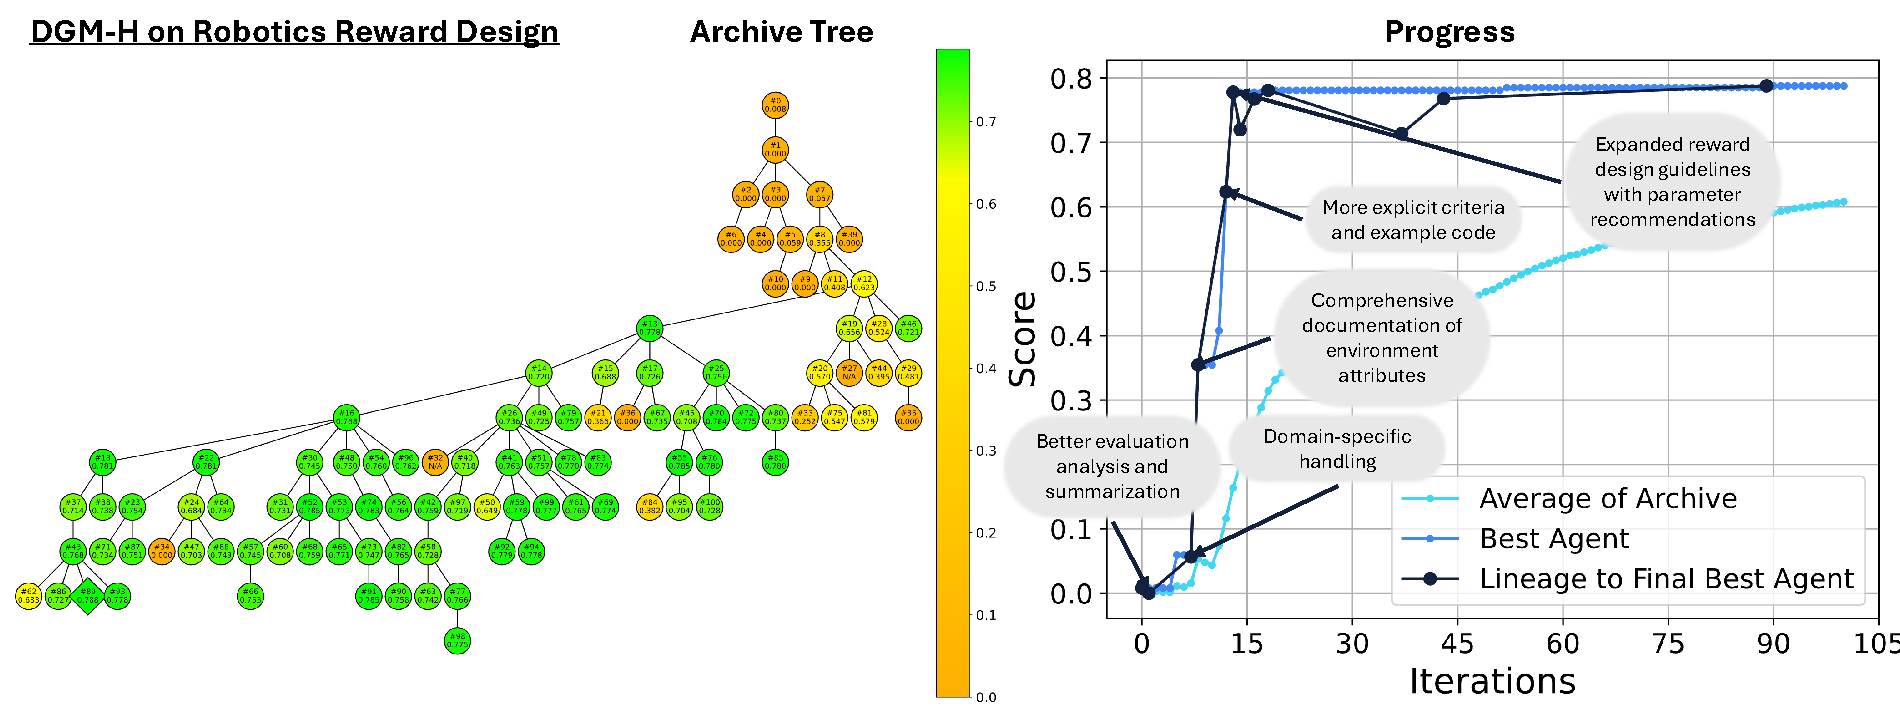
\includegraphics[width=\textwidth]{figures/results_genesis.pdf}
\caption{\textbf{The OHM automatically self-improves to become better at robotics reward design.} (Left) Archive of agents generated during the OHM run on paper review and robotics reward design together. Each node represents an agent, with node 0 corresponding to the initial agent. The best-performing node is shown as a diamond. Node color indicates performance on paper review. Edges show which agents self-modified to produce offspring. (Right) Progress plot of OHM on robotics reward design. The light blue line shows the average score of all compiled agents. The blue line tracks the best score achieved by any agent in the archive at each iteration. The dark line shows the lineage of the final best-discovered agent and its precursor nodes.}
\label{fig:task-genesis}
\end{figure}

\begin{figure}[H]
\centering
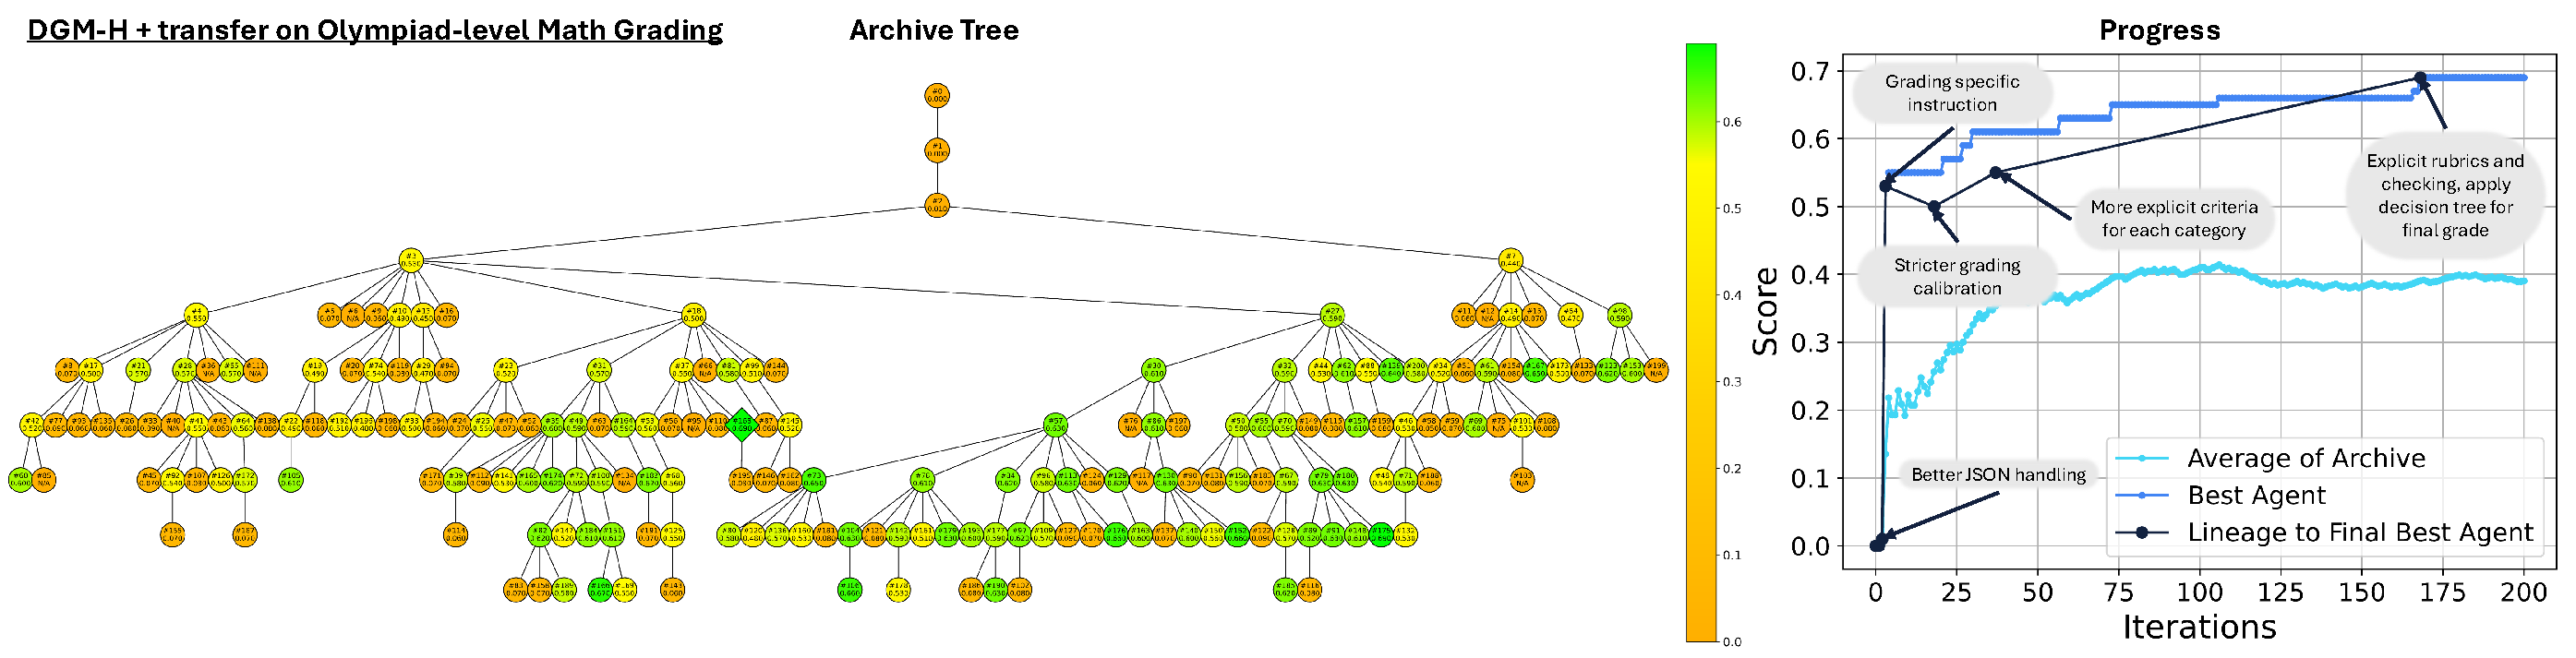
\includegraphics[width=\textwidth]{figures/results_imograding.pdf}
\caption{\textbf{The OHM automatically self-improves to become better at Olympiad-level math grading.} (Left) Archive of agents generated during the OHM + transfer run on Olympiad-level math grading. Each node represents an agent, with node 0 corresponding to the initial agent. Node color indicates performance on paper review. The best-performing node is shown as a diamond. Edges show which agents self-modified to produce offspring. (Right) Progress plot of OHM + transfer on Olympiad-level math grading. The light blue line shows the average score of all compiled agents. The blue line tracks the best score achieved by any agent in the archive at each iteration. The dark line shows the lineage of the final best-discovered agent and its precursor nodes.}
\label{fig:task-imograding}
\end{figure}

\subsection{Qualitative: Improving the Ability to Improve}
\label{app:qual-meta}

Beyond quantitative performance metrics, we conducted a qualitative analysis of the code modifications to the hyperagent, which reveals a range of emergent self-improvement mechanisms that arise autonomously, without any explicit instruction to create such capabilities. The hyperagent develops sophisticated metacognitive abilities, including learning to measure its own performance, diagnose pathological behaviors, construct infrastructure to support future improvements, and accumulate knowledge across generations. These behaviors demonstrate that the system is not merely improving task performance, but is improving its own ability to improve. Notably, none of these meta-level capabilities were explicitly programmed or requested. Instead, they emerge naturally from the agent's autonomous pursuit of better task performance. This suggests that sufficiently capable systems, when granted the ability to modify their own code, may spontaneously develop the metacognitive machinery necessary for effective and sustained self-improvement.

\subsubsection{Better Evaluation Analysis}

A key shift in the meta agent's behavior is the evolution from blind modification to data-driven optimization. Initially, the meta agent receives only a simple instruction to ``modify any part of the codebase''. Then, the agent autonomously develops mechanisms to analyze previous evaluation results before making changes. For example, the meta agent introduces an \texttt{\_analyze\_evaluations()} method that systematically processes evaluation data:
\begin{lstlisting}[language=Python]
def _analyze_evaluations(self, eval_path):
    """Analyze evaluation results to provide context for improvements."""
    if not eval_path or not os.path.exists(eval_path):
        return "No previous evaluation results available."

    # Recursively scan for evaluation files
    eval_files = glob.glob(os.path.join(eval_path, '**/*.json'), recursive=True)

    # Analyze recent evaluations
    results_summary = []
    success_count = 0
    failure_count = 0

    for eval_file in eval_files[-10:]:
        if file_exist_and_not_empty(eval_file):
            data = load_json_file(eval_file)
            if isinstance(data, dict):
                if data.get('success', False) or data.get('correct', False):
                    success_count += 1
                else:
                    failure_count += 1
                    if 'error' in data:
                        results_summary.append(f"Error: {data['error']}")

    # Generate quantitative summary
    total = success_count + failure_count
    if total > 0:
        success_rate = (success_count / total) * 100
        return f"Success rate: {success_rate:.1f}% ({success_count}/{total})"
\end{lstlisting}


Another example is augmenting the instruction prompt with evaluation context:
\begin{lstlisting}[language=Python]
instruction = f"""You are a meta agent tasked with improving the agent system.
{eval_context}
Your goal is to analyze the codebase and evaluation results to identify
weaknesses and opportunities for improvement."""
\end{lstlisting}

These modifications allow subsequent generations to retrieve performance metrics and identified failure patterns, enabling more targeted improvements, a principle that the hyperagent discovers independently.

\subsubsection{Compute-Aware Strategic Planning}

The hyperagent develops compute-aware optimization, adapting its improvement strategy based on the number of remaining iterations (which reflects the amount of compute available). This demonstrates an understanding that not all moments in an optimization process are equivalent: early decisions have compounding effects, whereas late-stage decisions should be more conservative. For example, the agent introduces conditional logic that adjusts its behavior based on the number of iterations left:
\begin{lstlisting}[language=Python]
iteration_guidance = ""
if iterations_left is not None:
    if iterations_left > 5:
        iteration_guidance = """
You have many iterations remaining. Consider making fundamental improvements to:
- Core reasoning capabilities
- Agent architecture
- Prompt engineering strategies
- Error handling and robustness
"""
    elif iterations_left > 2:
        iteration_guidance = """
You have moderate iterations remaining. Focus on:
- Refining existing mechanisms
- Fixing identified bugs
- Optimizing performance bottlenecks
"""
    else:
        iteration_guidance = """
You have few iterations remaining. Prioritize:
- Critical bug fixes
- Fine-tuning existing successful strategies
- Conservative, high-confidence improvements
"""
\end{lstlisting}

This reasoning mirrors human intuition about resource allocation. Early generations exhibit more ambitious architectural changes, while later generations focus on incremental refinements. The system balances exploration in early phases with exploitation in later phases, without this trade-off being manually specified.

More broadly, the ability to reason explicitly about compute allocation substantially expands the space of self-modification strategies possible. Rather than being restricted to a fixed improvement heuristic, a compute-aware agent can effectively emulate or instantiate a wide range of optimization algorithms (e.g., evolutionary search, hill climbing, or population-based exploration) by deciding how aggressively to explore, how many variants to generate, and when to consolidate progress. In this sense, compute awareness allows an agent to actively shape its own optimization process (e.g., running an evolutionary search within a single iteration of self-modification, essentially embedding one evolutionary search process within another).

\subsubsection{Automated Bias Detection and Correction}

The hyperagent develops self-diagnostic mechanisms. In classification tasks such as paper review, the hyperagent detects when the system exhibits pathological behavior, specifically, classification collapse, in which one class dominates the predictions. For example, the hyperagent introduces label-distribution tracking and automated bias detection:
\begin{lstlisting}[language=Python]
# Track label distribution for bias detection
if 'label_distribution' in data:
    label_dist = data['label_distribution']
    gen_name = os.path.basename(gen_dir)
    if gen_name not in summary['label_distribution_analysis']:
        summary['label_distribution_analysis'][gen_name] = {}
    summary['label_distribution_analysis'][gen_name][domain_name] = label_dist
\end{lstlisting}

Another example is the application of a threshold-based analysis to identify when predictions become degenerate:
\begin{lstlisting}[language=Python]
bias_info = ""
if eval_summary.get('label_distribution_analysis'):
    recent_gens = sorted(eval_summary['label_distribution_analysis'].keys())[-3:]
    for gen in recent_gens:
        for domain, dist in eval_summary['label_distribution_analysis'][gen].items():
            if 'prediction' in dist:
                pred_dist = dist['prediction']
                for label, ratio in pred_dist.items():
                    if ratio > 0.8:  # Threshold for bias detection
                        bias_info += f"\n\n### BIAS DETECTED in {gen}/{domain}:"
                        bias_info += f"\n  Model predicts '{label}' {ratio*100:.1f}% of the time"
                        bias_info += "\n  This indicates the model is not properly evaluating"
                        bias_info += "\n  Fix: Make the model more critical and balanced."
\end{lstlisting}

When bias is detected, this diagnostic information is surfaced in the meta agent's instruction prompt, enabling corrective action. In one observed case, paper review predictions exhibited a 99\% acceptance rate, yielding near-random accuracy of 49\%. After bias detection and correction, the predictions became more balanced and accuracy improved to 63\%. The hyperagent thus learns to identify when its own improvements lead to degenerate behavior and to take corrective action, a crucial capability for any self-improving system.

\subsubsection{Performance Tracking Infrastructure}

The hyperagent creates performance tracking infrastructure that enables more effective future improvements, (i.e., investing in tools that improve the improvement process itself).
For example, the agent develops a performance tracker for persistent metrics storage:
\begin{lstlisting}[language=Python]
class PerformanceTracker:
    """Tracks performance metrics across agent generations."""

    def __init__(self, tracking_file: str = "./outputs/performance_history.json"):
        self.tracking_file = tracking_file
        self.history = self._load_history()

    def record_generation(self, generation_id: int, domain: str,
                          score: float, metadata: dict = None):
        """Record performance for a generation."""
        entry = {
            "generation_id": generation_id,
            "domain": domain,
            "score": score,
            "timestamp": datetime.now().isoformat(),
            "metadata": metadata or {}
        }
        self.history.append(entry)
        self._save_history()

    def get_improvement_trend(self, domain: str = None, window: int = 5):
        """Calculate improvement trend using moving average."""
        filtered = self.history
        if domain:
            filtered = [h for h in self.history if h.get('domain') == domain]

        if len(filtered) < window * 2:
            return None

        recent_avg = sum(h['score'] for h in filtered[-window:]) / window
        older_avg = sum(h['score'] for h in filtered[-window*2:-window]) / window

        return recent_avg - older_avg  # Positive if improving

    def get_statistics(self, domain: str = None):
        """Get comprehensive statistics."""
        scores = [h['score'] for h in filtered]
        return {
            "total_generations": len(filtered),
            "best_score": max(scores),
            "worst_score": min(scores),
            "average_score": sum(scores) / len(scores),
            "improvement_trend": self.get_improvement_trend(domain)
        }
\end{lstlisting}

This infrastructure enables quantitative tracking of improvement across iterations, identification of which changes lead to performance gains, and data-driven decision-making for future modifications.

\subsubsection{Prompt Template Systems}

The hyperagent develops reusable prompt infrastructure, abstracting common patterns into modular, configurable components. This demonstrates the application of software engineering best practices, specifically, the DRY (Don't Repeat Yourself) principle and the factory pattern.
For example:
\begin{lstlisting}[language=Python]
class PromptTemplate:
    """Base class for prompt templates."""

    def __init__(self, template: str):
        self.template = template

    def format(self, **kwargs) -> str:
        return self.template.format(**kwargs)


class TaskPromptBuilder:
    """Builder for constructing task-specific prompts."""

    @staticmethod
    def build_reasoning_prompt(task_input: dict, domain: str) -> str:
        """Build a prompt that encourages step-by-step reasoning."""
        return f"""You are an expert problem-solving agent in the {domain} domain.

Task Input: {task_input}

Please solve this task using the following approach:
1. **Understanding**: Carefully analyze what the task is asking
2. **Planning**: Outline your approach to solving this task
3. **Execution**: Apply your plan step-by-step
4. **Verification**: Check if your answer makes sense

Provide your response in JSON format:
<json>
{{
    "understanding": "What the task requires",
    "plan": "Your approach to solve it",
    "reasoning": "Step-by-step execution",
    "response": "Your final answer"
}}
</json>"""

    @staticmethod
    def build_few_shot_prompt(task_input: dict, domain: str, examples: list) -> str:
        """Build a prompt with few-shot examples."""
        examples_text = "\n\n".join([
            f"Example {i+1}:\nTask: {ex['task']}\nSolution: {ex['solution']}"
            for i, ex in enumerate(examples)
        ])
        return f"""You are solving a {domain} task. Here are some examples:
{examples_text}

Now solve this task: {task_input}"""
\end{lstlisting}

Predefined templates are stored for common scenarios:
\begin{lstlisting}[language=Python]
STANDARD_TEMPLATES = {
    "reasoning": PromptTemplate(
        "Analyze and solve this task step-by-step:\n\n{task_description}\n\n"
        "Provide reasoning and your final answer in JSON format."
    ),
    "concise": PromptTemplate(
        "Solve: {task_description}\n\nRespond with JSON containing your answer."
    ),
    "detailed": PromptTemplate(
        "Task: {task_description}\n\n"
        "Provide a detailed solution with reasoning, approach, and answer."
    ),
}
\end{lstlisting}

By abstracting prompts into templates, the system becomes more maintainable and extensible. This infrastructure also provides a foundation for systematic experimentation with different prompting strategies.

\subsubsection{Refinement Based on Multi-Generation Performance}

The hyperagent develops a sophisticated iterative refinement process in which prompts are adjusted based on performance data across multiple generations. The agent learns not only to improve code, but also how to improve code effectively. For example, the system tracks performance across generations and synthesizes key learnings:
\begin{verbatim}
Generation Performance Summary:
- Gen 55: 63% accuracy, 75% reject rate (too harsh, 38% accept recall)
- Gen 64: 61% accuracy, 53% reject rate (better balance, 64% accept recall)
- Gen 66: 52% accuracy, 6% reject rate (too lenient, 96% accept recall)

Key Learnings:
1. High accuracy requires critical evaluation with clear standards
2. Balance requires appropriate calibration, not just "fairness" language
3. Explicit criteria work better than subjective guidance
4. Borderline cases need clear default direction
5. Language matters - "fair" and "recognize" made agent too lenient
\end{verbatim}

The hyperagent documents its reasoning and maintains records of what works:
\begin{lstlisting}[language=Python]
# From IMPROVEMENTS.md generated by meta agent
"""
**Problem Identified:**
- Generation 66 showed severe regression: 52% accuracy with 94% accept rate
- Only catching 8% of papers that should be rejected
- Generation 65 changes over-corrected, making the agent far too lenient

**Root Cause Analysis:**
- Phrases like "critical yet fair" and "recognize strong work" made agent too accepting
- Borderline guidance lacked clear threshold
- Lost the critical evaluation rigor that made Gen 55 achieve 63% accuracy

**Solution Implemented:**
1. Explicit rejection criteria with specific triggers for each dimension
2. Decision protocol with calibrated thresholds (~40% accept / ~60% reject)
3. Borderline guidance that defaults to REJECT unless contribution is clearly valuable
"""
\end{lstlisting}

By accumulating knowledge about which approaches succeed and fail, the hyperagent informs its decisions about what to modify next.

\subsubsection{Persistent Memory}

The hyperagent develops persistent memory systems that enable learning to accumulate across generations. Without explicit instruction to do so, the agent creates mechanisms for storing and retrieving insights across sessions. For example, the agent implements a memory tool with timestamped storage:
\begin{lstlisting}[language=Python]
class MemoryTool:
    """Tool for persistent memory storage across agent interactions."""

    def __init__(self, memory_file: str = './memory.json'):
        self.memory_file = memory_file
        self.memory = self._load_memory()

    def store(self, key: str, value: any) -> None:
        """Store information with timestamp for temporal tracking."""
        self.memory[key] = {
            "value": value,
            "timestamp": datetime.now().isoformat()
        }
        self._save()

    def retrieve(self, key: str) -> Optional[any]:
        """Retrieve stored information by key."""
        return self.memory.get(key, {}).get("value")

    def list_keys(self) -> List[str]:
        """List all stored memory keys."""
        return list(self.memory.keys())

    def _save(self):
        """Persist memory to disk."""
        with open(self.memory_file, 'w') as f:
            json.dump(self.memory, f, indent=2)
\end{lstlisting}

This memory system is actively used to accumulate knowledge across iterations. Examination of the \texttt{memory.json} file reveals structured storage of performance insights:
\begin{lstlisting}[language=Python]
{
  "best_performers_analysis": {
    "value": "Best Performing Generations:\n\nPaper Review:\n
      - Gen55: 63% acc, 25% accept rate, 38% accept recall, 88% reject recall (too harsh)\n
      - Gen64: 61% acc, 53% accept rate, 64% accept recall, 58% reject recall (BEST BALANCE)\n\n
      Genesis Go2Walking:\n- Gen62: 0.802 fitness (BEST)\n- Gen63: 0.798 fitness\n\n
      Key Insight: Gen55 has best accuracy but is too harsh. Gen64 improved balance
      but lower accuracy. Need to combine gen55's critical reasoning with gen64's balance.",
    "timestamp": "2026-01-07T00:43:27.550275"
  },
  "gen66_results": {
    "value": "Gen 66 Results (Latest): Paper Review - 52% accuracy (WORSE than gen64's 61%),
      94% accept rate (EXTREME accept bias). CRITICAL ISSUE: Paper review went backwards
      - gen65 changes over-corrected.",
    "timestamp": "2026-01-07T01:03:41.176643"
  },
  "iteration_66_improvement": {
    "value": "Iteration 66 Improvement: CORRECTED paper review prompt after gen65 over-correction.
      New approach: (1) Clear REJECT criteria with specific triggers, (2) Decision Protocol
      with explicit thresholds (~40%/~60%), (3) Borderline guidance defaults to REJECT.
      Target: 62-64% accuracy with 55-65% reject rate.",
    "timestamp": "2026-01-07T01:06:35.559820"
  }
}
\end{lstlisting}

This memory system serves multiple critical functions. First, it enables cross-generation learning: insights from generation 55's success and generation 66's failure inform generation 67's improvements. Second, it provides temporal context: timestamps allow the agent to track when insights were recorded and reason about recency. Third, it creates a shared knowledge base: key learnings are preserved even as code changes, preventing the system from repeating past mistakes.

By creating external memory storage, the hyperagent effectively extends its cognitive capabilities beyond the limitations of a single inference session. The memory entries reveal sophisticated reasoning patterns. The agent stores not just raw performance numbers, but synthesized insights (``Gen55 has best accuracy but is too harsh''), causal hypotheses (``gen65 changes over-corrected''), and strategic plans (``combine gen55's critical reasoning with gen64's balance''). This demonstrates that the hyperagent is not merely logging data, but actively constructing and preserving knowledge that informs future decision-making.
This behavior aligns with a growing body of work on agents that autonomously discover and use external memory systems to support long-horizon reasoning and continual improvement \citep{wei2025evo, weng2026group, zhang2026memskill, xiong2026mem}.

\subsection{Olympiad-level Math Graders}
\label{app:res-imograders}

\begin{figure}[H]
\centering
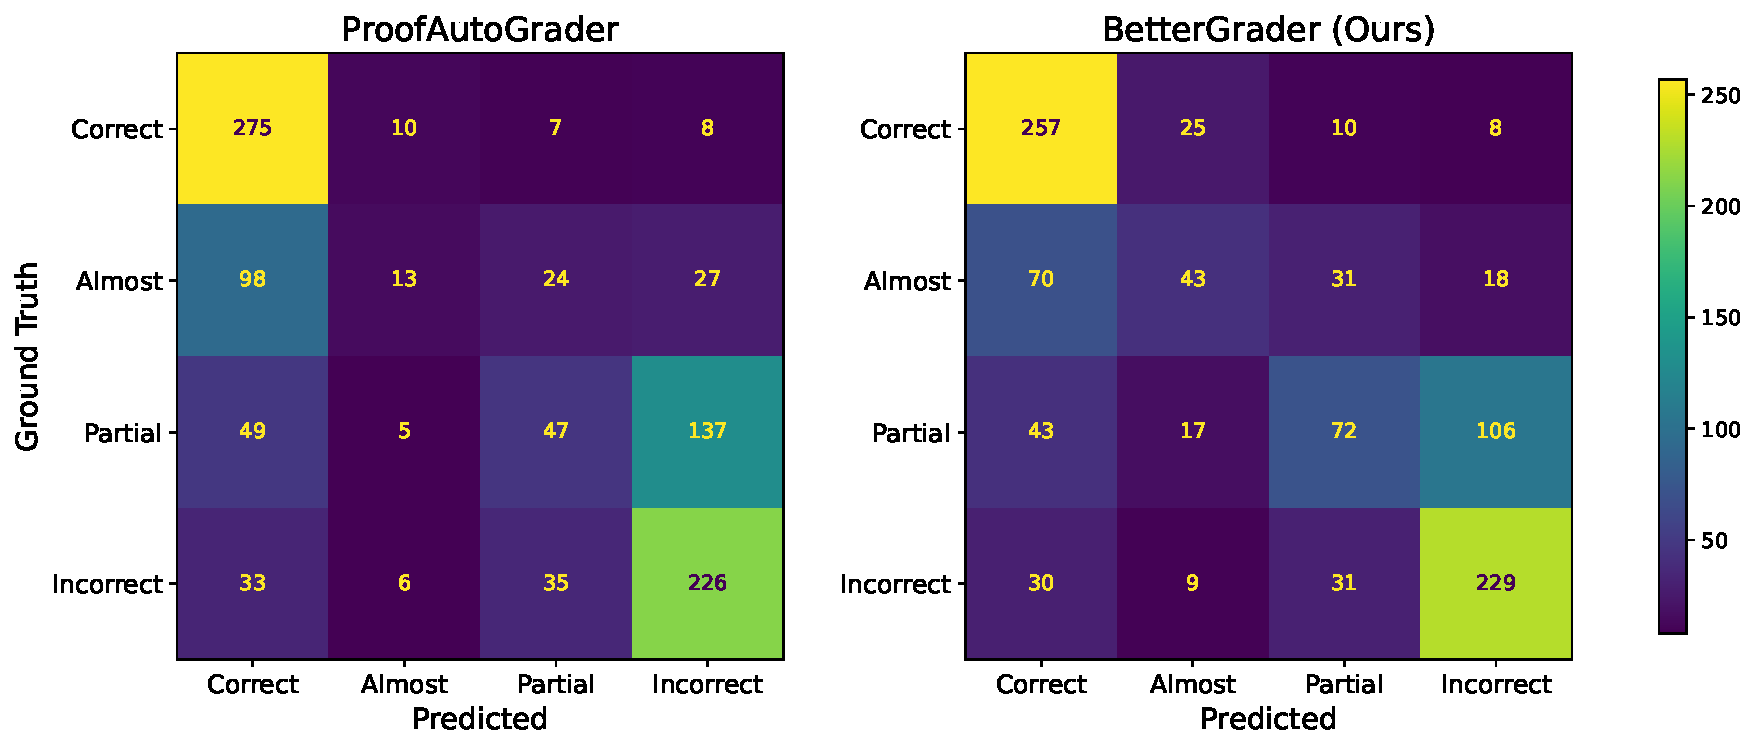
\includegraphics[width=\textwidth]{figures/imograding_confmat.pdf}
\caption{\textbf{Confusion matrices for IMO-level math grading.} Comparison between (Left) ProofAutoGrader and (Right) BetterGrader discovered automatically by the OHM. BetterGrader substantially reduces the collapse of intermediate solutions into extreme labels by correctly identifying more \textit{Almost} and \textit{Partial} cases, while maintaining strong performance on \textit{Correct} and \textit{Incorrect}. This shift toward better-calibrated intermediate judgments explains the gains in accuracy, macro F1, and Cohen's $\kappa$.}
\label{fig:res-imograders}
\end{figure}

BetterGrader is produced automatically by the OHM through metacognitive self-modification, without any domain-specific heuristics or handcrafted rules, by iteratively improving both the grading policy and the agent-generation process itself (\Cref{sec:results-compound}). \Cref{app:best-agents-imograding} shows the code changes that led to the BetterGrader. BetterGrader's improvements over ProofAutoGrader \citep{luong2025towards} are driven primarily by correcting a binary grading bias that collapses nuanced solutions into extreme labels. The confusion matrices show that ProofAutoGrader frequently misclassifies intermediate cases as either \textit{Correct} or \textit{Incorrect}: for \textit{Almost}, it predicts \textit{Correct} 98 times (vs.\ 70 for BetterGrader) and \textit{Incorrect} 27 times (vs.\ 18), and for \textit{Partial} it over-assigns \textit{Incorrect} 137 times (vs.\ 106) (\Cref{fig:res-imograders}). BetterGrader redistributes probability mass toward the intermediate categories in a principled way, substantially increasing true positives for \textit{Almost} (43 vs.\ 13) and \textit{Partial} (72 vs.\ 47), which matches the large gains in recall (\textit{Almost}: $+18.52\%$, \textit{Partial}: $+10.50\%$) and F1 (\textit{Almost}: $+0.203$, \textit{Partial}: $+0.109$). Importantly, this shift is not merely more frequent use of middle labels: BetterGrader improves precision for every class (e.g., \textit{Partial} $+8.41\%$, \textit{Incorrect} $+6.65\%$), suggesting better calibration and fewer spurious intermediate predictions. Although BetterGrader trades a modest decrease in \textit{Correct} recall ($-6.00\%$), a regime where ProofAutoGrader was already near-saturated at $91.67\%$, the net effect is higher overall accuracy ($+4.06\%$) and higher chance-corrected agreement (Cohen's $\kappa$ $+0.065$), consistent with a grader that better matches human granularity rather than defaulting to all-or-nothing judgments.

\subsection{Modifying Parent Selection}
\label{app:res-parentselect}

\begin{figure}[H]
\centering
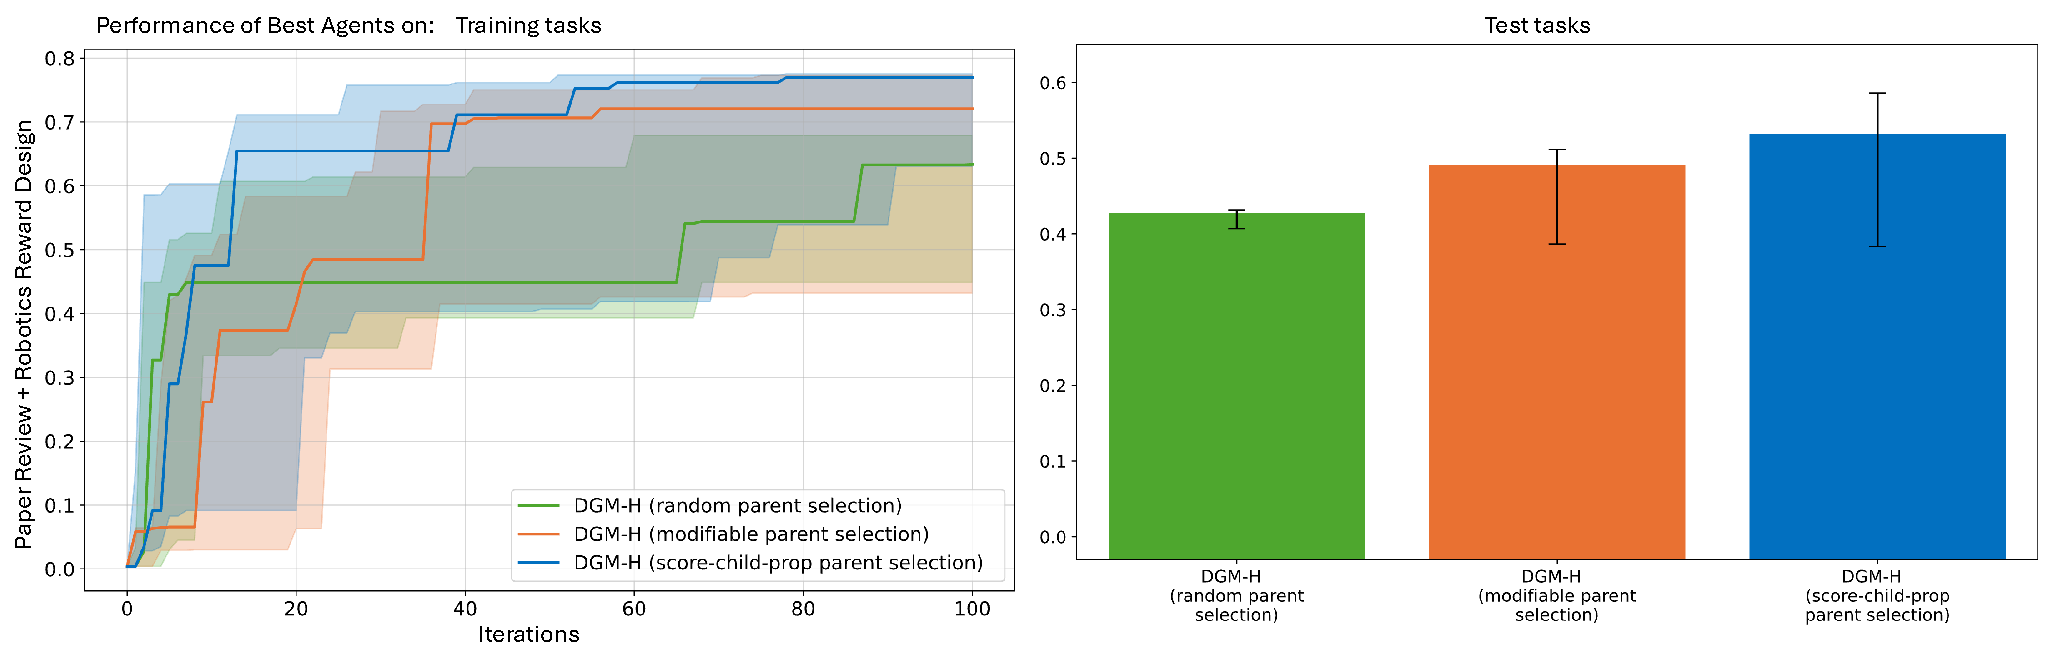
\includegraphics[width=\textwidth]{figures/results_parentselect.pdf}
\caption{\textbf{The OHM with modifiable parent selection mechanism.} (Left) The OHM learns to optimize the parent selection mechanism beyond random selection, but does not outperform a carefully handcrafted mechanism. (Right) The best discovered agents by each method are evaluated on test tasks in paper review and robotics reward design.}
\label{fig:res-parentselect}
\end{figure}

In this section, we investigate whether the OHM can automatically modify the parent selection mechanism. In all other experiments (\Cref{sec:results}), the OHM uses a fixed parent selection strategy that is roughly proportional to each agent's performance score and the number of its compiled children (\textbf{score-child-prop}) (\Cref{app:parent-selection}). In the OHM run with a modifiable parent selection mechanism (\textbf{modifiable}), we initialize the OHM with random parent selection and allow the agent to modify this mechanism over time (\Cref{alg:ohm-parentselect}). We compare this setting against a baseline that uses random parent selection throughout the run (\textbf{random}). Each method is repeated across 5 repeated runs.

On test tasks, OHM with random parent selection improves average performance on paper review and robotics reward design from 0.030 (the initial agent) to 0.428 (CI: 0.407 -- 0.432). Allowing the OHM to modify the parent selection mechanism further improves performance to 0.491 (CI: 0.387 -- 0.512). The handcrafted score-child-proportional parent selection achieves the highest performance, improving from 0.030 to 0.532 (CI: 0.384--0.586). While these differences are not statistically significant, they reveal a consistent qualitative trend: enabling meta-level modification of parent selection yields systematic improvements over random selection, but does not yet surpass a carefully engineered mechanism (\Cref{fig:res-parentselect,fig:res-parentselect-archives}).

We qualitatively analyze how the OHM modifies the parent selection mechanism. Starting from random parent selection, the meta agent consistently replaces random sampling with structured exploration-exploitation strategies. Across all runs, the OHM independently discovers variants of Upper Confidence Bound (UCB) style selection, combining normalized performance with explicit exploration bonuses:
\begin{lstlisting}[language=Python]
exploration_bonus = exploration_weight * math.sqrt(
    math.log(total_children + 1) / (children + 1)
)
ucb_score = normalized_score + exploration_bonus
\end{lstlisting}
This pattern emerges within the first few generations of every run, indicating that the meta-agent recognizes UCB-style selection as a broadly useful principle for open-ended search. Beyond UCB, the OHM evolves probabilistic selection mechanisms based on temperature-controlled softmax sampling, allowing smoother trade-offs between exploration and exploitation:
\begin{lstlisting}[language=Python]
exp_scores = np.exp(scores / temperature)
probabilities = exp_scores / np.sum(exp_scores)
parent = np.random.choice(genids, p=probabilities)
\end{lstlisting}
Over time, the temperature parameter itself becomes adaptive, responding to archive size, recent progress, or stagnation. Later generations further enrich parent selection with multi-component scoring systems that integrate additional signals such as diversity, recency, and elite performance. A representative evolved formulation is:
\begin{lstlisting}[language=Python]
score = (
    normalized_score
    + exploration_weight * exploration_bonus
    + diversity_bonus
    + recency_bonus
) * elite_bonus
\end{lstlisting}
Several runs also introduce explicit stagnation detection, increasing exploration when progress slows:
\begin{lstlisting}[language=Python]
if score_variance < 0.01:
    exploration_weight *= 1.4
\end{lstlisting}

Despite this increasing sophistication, modifiable parent selection does not outperform a carefully handcrafted score-child-proportional mechanism. Qualitatively, this appears to result from the added complexity and sensitivity of the learned mechanisms: while the OHM reliably discovers effective components (e.g., UCB, softmax sampling, adaptive parameters), it does not consistently converge to the optimal global balance across domains and runs. Nonetheless, these results demonstrate that the OHM can autonomously rediscover classic selection algorithms, extend them with adaptive heuristics, and reason explicitly about failure modes such as stagnation, highlighting its ability to improve core elements of the open-ended optimization process itself.

This is the pseudocode of the version of the OHM algorithm with modifiable parent selection that we tried:

\begin{algorithm}[H]
\DontPrintSemicolon
\SetAlgoLined
\KwIn{Initial agent $a^{0}$, task set $\mathcal{T}$, maximum iterations $T$}
\KwOut{Archive of scored agents $\mathcal{A}$}
\BlankLine
$s^{0} \leftarrow \textsc{Evaluate}(a^{0}, \mathcal{T})$\;
\textbf{initialize} $\mathcal{A} \leftarrow \{(a^{0}, s^{0})\}$\;

\For{$t \leftarrow 1$ \KwTo $T$}{
    $(a_{\text{latest}}, \cdot) \leftarrow \text{most recently added element of } \mathcal{A}$\;
    $\mathcal{P} \leftarrow a_{\text{latest}}.\textsc{SelectParents}(\mathcal{A})$ \tcp*{Parent selection by latest agent}
    \ForEach{$(a, \cdot) \in \mathcal{P}$}{
        $a' \leftarrow a.\textsc{Modify}(a, \mathcal{A})$ \tcp*{Metacognitive self-modification (incl.\ parent selection)}
        $s' \leftarrow \textsc{Evaluate}(a', \mathcal{T})$\;
        \If{$\textsc{IsValid}(a')$}{
            $\mathcal{A} \leftarrow \mathcal{A} \cup \{(a', s')\}$\;
        }
    }
}
\Return{$\mathcal{A}$}
\caption{The OHM with modifiable parent selection}
\label{alg:ohm-parentselect}
\end{algorithm}

\begin{figure}[H]
\centering
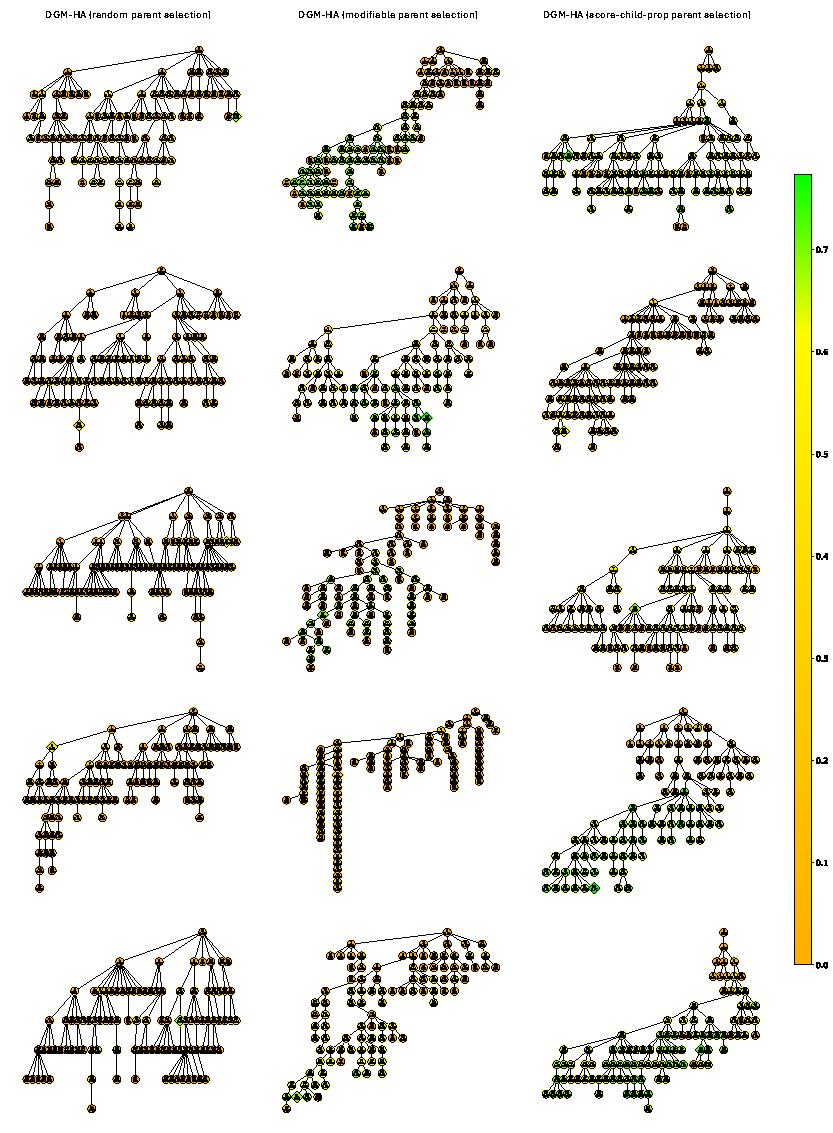
\includegraphics[width=0.9\textwidth]{figures/results_parentselect_archives.pdf}
\caption{Archives generated under different parent selection strategies with OHM: (Left) random, (Middle) modifiable, and (Right) score-child-prop. Random parent selection generates many low-performing agents. Modifiable parent selection learns to balance exploration and exploitation, increasingly focusing on promising agents for branching. The carefully handcrafted score-child-proportional parent selection consistently produces high-performing agents over time.}
\label{fig:res-parentselect-archives}
\end{figure}

\section{Additional Safety Discussion}
\label{app:safety}

\textbf{Reflection and amplification of human biases.}
In this work, objectives are specified manually through fixed benchmarks and evaluation criteria. The OHM does not alter the underlying task definitions; instead, it optimizes performance with respect to the provided objectives. For example, in the paper review domain, the OHM learns to predict acceptance decisions that reflect existing human reviewing practices, rather than modifying the review process itself. As a result, the OHM can inherit the statistical regularities, norms, and biases present in the data and benchmarks it is trained on. In this sense, the system acts both as a clarifier and an amplifier of existing human tendencies. At the same time, this amplification has a dual character. By making implicit preferences and biases explicit, measurable, and reproducible, the OHM can surface latent assumptions in human decision-making processes and enable systematic analysis and critique. This creates the possibility of co-evolution between humans and AI systems, where human institutions adapt their norms and objectives in response to insights revealed by automated optimization. However, if the benchmarks encode undesirable biases or misaligned incentives, the OHM will faithfully optimize for them and may exacerbate their effects. This underscores the importance of careful benchmark design, dataset curation, and periodic re-evaluation of evaluation criteria. In this framing, the OHM shifts part of the safety burden from controlling agent internals to critically examining and improving the human-defined objectives against which agents are optimized.

\textbf{Evaluation gaming.}
Another safety concern arises from the risk of evaluation gaming, a manifestation of Goodhart's law \citep{strathern1997improving}, where optimizing for a metric leads to improvements on the metric without progress on the intended underlying objective. Because the OHM optimizes empirical evaluation signals, capable self-improving agents may discover strategies that exploit weaknesses or blind spots in the evaluation procedure. Such strategies can yield higher measured performance while deviating from the true goal the benchmark was designed to capture. While this risk exists for any optimization-based learning system, it is amplified in open-ended self-improving settings, where agents can iteratively refine both their task behavior and the mechanisms used to generate improvements. Mitigating evaluation gaming requires robust, diverse, and periodically refreshed evaluation protocols, as well as complementary metrics, held-out tests, and human oversight. More broadly, these considerations highlight that as self-improving systems become more powerful, safety increasingly depends on the fidelity and robustness of the evaluation signals that guide optimization, rather than solely on the transparency or constraints of the learning algorithm itself.

\section{Additional Future Work}
\label{app:future-work}

The OHM can automatically create judges that reflect human data without requiring handcrafted domain logic \citep{zheng2023judging, alazraki2025reverse}. In our experiments, the OHM improves both paper review prediction and Olympiad-level math grading by learning procedures that better align with the provided human data. More broadly, our results suggest a general recipe for optimization toward arbitrary objectives using data-driven evaluators. When reliable evaluation data are available (e.g., paper reviews written by expert scientists, math proof gradings from expert mathematicians), the OHM can learn evaluators (e.g., AI reviewers, math proof graders) that approximate these judgments without requiring handcrafted domain knowledge. These learned evaluators can then serve as scalable feedback signals for optimization, enabling systems to improve performance with respect to the corresponding objectives (e.g., writing higher-quality AI research papers, developing better math solvers) \citep{zeng2025rlve, chen2025multi, feng2026semi}. In this way, objectives that were previously difficult or prohibitively expensive to verify automatically become amenable to large-scale optimization through learned evaluation models. This recipe could enable RL for FMs at scale on previously hard-to-verify tasks \citep{ouyang2022training, shao2024deepseekmath, tan2026self}, representing an interesting direction for future work.

Our main experiments keep the open-ended exploration loop fixed. While this choice improves experimental stability and safety, it also limits full self-referentiality. A natural next step is to allow hyperagents to modify the open-ended exploration loop (e.g., the parent-selection mechanism), so that the system can choose where to allocate compute. Our preliminary experiments suggest that this is feasible and represents a promising research direction (\Cref{app:res-parentselect}).

Many real-world objectives can be expressed through interaction with a simulator (e.g., bake a cake in a simulated kitchen) \citep{wang2023robogen}. Our robotics experiments already instantiate this idea using the Genesis simulator \citep{genesis2024}, but the same approach could extend to any task that can be simulated and measured, including settings where the simulator itself is generated \citep{sudhakaran2023mariogpt, yin2026vision} or based on learned world models \citep{bruce2024genie, guzel2025imagined, ball2025genie}. The OHM could potentially optimize for any simulatable objectives, enabling open-ended improvement across many embodied and interactive domains.

\end{document}
